%%%%%Präambel%%%%%

\documentclass[12pt,a4paper]{report}%Schriftgröße, Papierformat einstellen
%\documentclass{scrbook}
\usepackage[top=30mm,bottom=30mm]{geometry}
\usepackage{lipsum}
\usepackage{csquotes}
%Pakete laden zur deutschen Rechtschreibung und für Umlaute
\usepackage[T1]{fontenc}
\usepackage[ngerman]{babel}
\usepackage[utf8]{inputenc} %für Windows, Linux
%\usepackage[applemac]{inputenc} %für Mac
%\usepackage{xcolor}
\usepackage[official]{eurosym}
\usepackage{graphicx}
\usepackage{caption}
\usepackage[dvipsnames]{xcolor}
\usepackage{cancel}
\usepackage{titlesec}
\usepackage{cite}
\usepackage{filecontents}
\usepackage{tabularx}
\usepackage{harvard}
\usepackage{units}
\usepackage{longtable} 
\usepackage{multirow}
\usepackage{chngcntr}
\usepackage{stmaryrd}
\usepackage{array}
\usepackage{autobreak}
\usepackage{booktabs}
\usepackage{float}
\usepackage{wrapfig}
\usepackage{hhline}
\let\harvardleftorig\harvardleft
%\usepackage[round]{natbib}
%\usepackage{hyperref}
\usepackage[nottoc,numbib]{tocbibind}
\usepackage[nottoc]{tocbibind}
\usepackage{siunitx}
\usepackage{esvect}
\usepackage{trfsigns}

%Pakete laden zu mathematischen Symbolen etc.
\usepackage{calc} 
\usepackage{amsmath,amssymb,amsthm,amsopn}
\usepackage{scrpage2}
\pagestyle{scrheadings}
\clearscrheadfoot
\automark[chapter]{section}
\ofoot{\pagemark}
\ifoot{}
\chead{\headmark}
\setfootsepline{1pt}
\setheadsepline{1pt}
%\setheadsepline[\textwidth+20pt]{0.5pt}

%Inhaltsverzeichnis mit Links erstellen
\usepackage[colorlinks,
pdfpagelabels,
pdfstartview = FitH,
bookmarksopen = true,
bookmarksnumbered = true,
linkcolor = black,
plainpages = false,
hypertexnames = false,
citecolor = black] {hyperref}

\setcounter{secnumdepth}{4}
\setcounter{tocdepth}{4}

\titleformat{\paragraph}
{\normalfont\normalsize\bfseries}{\theparagraph}{1em}{}
\titlespacing*{\paragraph}
{0pt}{3.25ex plus 1ex minus .2ex}{1.5ex plus .2ex}

\newcommand{\subsubsubsection}{\paragraph}

%mainly helping my laziness to flourish

%Makros
%Makro Color
%#1 Text
\def\colBord#1{\begingroup\color{Fuchsia}{#1}\endgroup}
\def\colRed#1{\begingroup\color{Red}{#1}\endgroup}
\def\colGreen#1{\begingroup\color{LimeGreen}{#1}\endgroup}
\def\colBlue#1{\begingroup\color{NavyBlue}{#1}\endgroup}

\def\usGreen#1#2{\underset{\colGreen{#1}}{#2}}
\def\usBord#1#2{\underset{\colBord{#1}}{#2}}

\def\ubGreen#1#2{\underbrace{#2}_{\colGreen{#1}}}

\def\|{\;|\;}
\def\ssum{ \sum_{k=1}^n}

%Some stuff i just dont wanna write everytime
\def\fermi{Fermi-Dirac-Verteilung}
\def\ul#1{\underline{#1}}
\def\€{\euro{}}
\def\epsF{\pmb{\varepsilon}}

\newcommand{\leftRightsection}[2]{
\begin{minipage}[t]{0.5\linewidth}
	\flushleft
	\textbf{#1}
\end{minipage}
	\hfill
\begin{minipage}[t]{0.4\linewidth}
	\flushright
	\textbf{#2}
\end{minipage}
}
\newcommand{\dottedSection}[2]{
\begin{minipage}[t]{0.95\linewidth}
	\textbf{#1 \dotfill #2}
	\end{minipage}
}
%This file contains loosely and not sorted math definitions...

\DeclareMathOperator{\grad}{grad}
\DeclareMathOperator{\diverg}{div}
\DeclareMathOperator{\rot}{rot}
\DeclareMathOperator{\spur}{spur}
\DeclareMathOperator{\determ}{det}

% Umgebungen für Definitionen, Sätze, usw.
\newtheorem{satz}{Satz}[section]
\newtheorem{definition}[satz]{Definition}     
\newtheorem{lemma}[satz]{Lemma}	
\newtheorem{bem}{Bemerkung}[section]
\newtheorem{bsp}{Beispiel}[section]
% Es werden Sätze, Definitionen etc innerhalb einer Section mit
% 1.1, 1.2 etc durchnummeriert, ebenso die Gleichungen mit (1.1), (1.2) ..                  
\numberwithin{equation}{section}


%neue Befehle definieren
\newcommand{\R}{\mathbb{R}} %zB \R als Abkürzung für das Symbol der reellen Zahlen
\newcommand{\N}{\mathbb{N}}
\newcommand{\Z}{\mathbb{Z}}
\newcommand{\Q}{\mathbb{Q}}
\newcommand{\C}{\mathbb{C}}
\newcommand{\diffp}{\partial}
\newcommand{\lapl}{\Delta}
%\def\lapl{\Delta}
%\newcommand{\diverg}{\operatorname{div}}

\def\vecT#1{\left(\begin{array}{c} #1 \end{array}\right)}
\def\dddot{\cdot \\ \cdot \\ \cdot}
\def\vecD#1{\vecT{#1_1 \\ \dddot \\ #1_d}}
\def\vecDt#1#2{\vecT{#1 \\ \dddot \\ #2}}
\def\vecN{\mathcal{O}}
\def\vspan#1{span \lbrace #1 \rbrace}
\def\vdim#1{dim \lbrace #1 \rbrace}
\def\vker#1{ker \lbrace #1 \rbrace}
\def\vrang#1{Rang \lbrace #1 \rbrace}
\def\mzxz#1#2#3#4{\left(\begin{array}{c c} #1 & #2 \\ #3 & #4 \\ \end{array}\right)}
\def\mdxd#1#2#3{\left(\begin{array}{c c c} #1 \\ #2 \\ #3 \end{array}\right)}
\def\dfp#1#2{\frac{\partial #1}{\partial #2}}
\def\diff#1#2{\frac{\mathrm{d}#1}{\mathrm{d}#2}}


\def\inR#1{\qquad ,\; #1 \in \R}
\def\inRs{\in \R}
\def\bracks#1{\left[ #1 \right]}
\def\abs#1{\left| #1 \right|}
\def\brac#1{\left( #1 \right)}
\def\dx{\;dx}
\def\dy{\;dy}
\def\dz{\;dz}
\def\dX{\;d\vec{x}}
\newcommand\citevgl
{\def\harvardleft{(vgl.\ \global\let\harvardleft\harvardleftorig}%
 \cite
}
\newcommand\citeVgl
{\def\harvardleft{(Vgl.\ \global\let\harvardleft\harvardleftorig}%
 \cite
}


\def\ccite#1#2{\glqq #1\grqq\cite{#2}}


\def\ezQu#1{'#1'}

\newcolumntype{L}[1]{>{\raggedleft\let\newline\\\arraybackslash\hspace{0pt}}m{#1}}

\def\multiTwo#1#2{\multicolumn{2}{>{\hsize=\dimexpr2\hsize+2\tabcolsep+\arrayrulewidth\relax}#1}{#2}}
\def\multiThree#1#2{\multicolumn{3}{>{\hsize=\dimexpr3\hsize+4\tabcolsep+2\arrayrulewidth\relax}#1}{#2}}

\newcolumntype{L}[1]{>{\raggedleft\let\newline\\\arraybackslash\hspace{0pt}}m{#1}}
\newcolumntype{R}[1]{>{\raggedright\let\newline\\\arraybackslash\hspace{0pt}}m{#1}}
\newcolumntype{P}[1]{>{\centering\arraybackslash}p{#1}}

\def\formTab#1#2{
\begin{equation}
  \begin{tabularx}{12cm}{R{3cm} l l}
    #1 &: &$#2$
  \end{tabularx}
\end{equation}
}
\newcommand{\formTabL}[3]{
\begin{equation}
  \begin{tabularx}{12cm}{R{3cm} l l}
    #1 &: &$#2$ 
  \end{tabularx}
  \label{eq:#3}
\end{equation}}
\def\formTn{$ \\ $\;$ & $\;$ & $}
\def\formTnQ{$ \\ $\;$ & $\;$ & $\qquad}
\def\formTnQQ{$ \\ $\;$ & $\;$ & $\qquad \qquad}
\def\formTnQQQ{$ \\ $\;$ & $\;$ & $\qquad \qquad \qquad}


\newcommand{\tabitem}{~~\llap{\textbullet}~~}

\renewcommand{\theequation}{\arabic{section}.\arabic{subsection}
.\arabic{equation}}
%Setzt den equation-Zaehler nach jeder Seite zurueck
%\numberwithin{equation}{subsection}	
\numberwithin{equation}{section}
%\setlength\abovedisplayskip{0pt}


%jetzt beginnt das eigentliche Dokument
\begin{document}
\bibliographystyle{agsm}

\author{}
\title{\underline{HM1-2 Kurzzusammenfassung} \\ $\;$ \\ $\;$ \\ Florian Leuze}
\date{}
\maketitle % erzeugt den Kopf

$\;$ \newline
$\;$ \newline
$\;$ \newline
$\;$ \newline
$\;$ \newline
$\;$ \newline
$\;$ \newline
$\;$ \newline
$\;$ \newline
$\;$ \newline
$\;$ \newline
$\;$ \newline
\begin{table}[H]
  \centering
  \begin{tabular}{P{14cm}}
    \begin{LARGE}
		  \glqq Mathematik zu lernen heißt,
    \end{LARGE}\\
    \begin{LARGE}
		   sie immer wieder neu zu erfinden.\grqq
    \end{LARGE}\\
    \begin{large}
      (Donal O'Shea)
    \end{large}
  \end{tabular}
\end{table}
\newpage
\tableofcontents

\section*{Versionierung}
\begin{tabular}{|p{2cm}|p{1cm}|p{1.5cm}|p{8.5cm}|}\hline
    Datum & Vers. & Kürzel & Änderung \\ \hline
    19.04.2018 & 0.1 & FL & Erzeugung Dokument; Erzeugung Inhaltsverzeichnis; Erzeugung Versionierung; Erzeugung 2.1 - 2.7.4 \\ \hline
    19.04.2018 & 0.2 & FL & Korrekturen 2.6.1 - 2.6.9 u. 2.7.1 - 2.7.2 Titel\\ \hline
    20.04.2018 & 0.2.1 & FL & Erzeugung 2.7.1.1 - 2.7.1.4; Korrektur Riemannsche Untersumme; Erzeugung Literaturverzeichnis \\ \hline
    01.05.2018 & 0.2.2 & FL & Neustrukturierung; Erzeugung Allgemeines; Erzeugung Zahlen \\ \hline
    23.06.2018 & 0.2.3 & FL & Neustrukturierung; Löschung HM1 Stoff; Erzeugung HM2 Stoff \\ \hline
    23.06.2018 & 0.2.4 & FL & Kleinere Korrekturen \\ \hline
    27.06.2018 & 0.2.5 & FL & Hinzugefügt: Bem. 2.8, 3.1, 3.2, 3.3, 3.8, 3.9.1 Schritt 5, 3.9.2 (Quadriken im $\R^2$; Korrekturen: 3.6.1.1 Fehler in Formel korrigiert, 3.6.1.3 Tippfehler korrigiert \\ \hline
    27.06.2018 & 0.2.6 & FL &  Bem. 3.6 korrigiert \\ \hline
    01.08.2018 & 0.3.0 & FL & Überarbeitung Trigonometrie \\ \hline
    04.08.2018 & 0.3.1 & FL & Erzeugung lin. skal. Diffgleichungen, LGS \\ \hline
    05.08.2018 & 0.3.2 & FL & Erzeugung Analytische Geometrie; Erzeugung Logik und Beweise \\ \hline
    06.08.2018 & 0.3.3 & FL & Erzeugung Mengen, Relationen und Abbildungen, Erzeugung konvergente Folgen \\ \hline
    07.08.2018 & 0.3.4 & FL & Erzeugung el. realw. Funktionen, Ableitung; Fertigstellung konvergente Folgen \\ \hline
    08.08.2018 & 0.3.5 & FL & Erzeugung Ableitung, Taylorpolynome und Reihen. \\ \hline
    09.08.2018 & 0.4.0 & FL & Umordnung von Reihen, Stetigkeit, Extremalprobleme, Funktionenfolgen; Korrekturen am Layout \\ \hline
    09.08.2018 & 0.4.2 & FL & Korrekturen am Layout \\ \hline
    09.08.2018 & 0.4.3 & FL & Korrektur Def.7.8 \\ \hline
    13.08.2018 & 0.3 & FL & Erzeugung Mehrd. Extremw., Satz über impl. Funkt., Extremwertaufgaben mit Nebenbe., Kurven/Bogenl., Wegintegrale \\ \hline
    13.08.2018 & 0.3.1 & FL & Kleinere Korrekturen \\ \hline
    13.08.2018 & 0.3.2 & FL & Korrektur Layout \\ \hline
   15.12.2018 & 0.3.3 & FL & Kleinere Korrekturen \\ \hline
   13.03.2019 & 1.0 & FL & Cleaned up, implemented proper structure, modularised  code, added quote, slighty changed format \\ \hline
  \end{tabular}
\listoffigures


%
%%first chapter damn im too lazy to think about some good notes to put here
\chapter{Allgemeines} 
	\section{Integralberechnung}
\subsection{Unbestimmtes Integral}
\begin{equation}
\int f(x) dx = F(x) + C = [F(x)]\qquad, C\in\R \label{eq:def_noBorder}
\end{equation}

\subsection{Bestimmtes Integral}
\begin{equation}
\int_a^b f(x) dx = F(b) - F(a) \label{eq:def_border}
\end{equation}

\subsection{Partielle Integration}
Entspricht der "Produktregel" der Differentialrechnung.
\begin{equation}
\int_{\colBord{a}}^{\colBord{b}} f'(x) g(x) dx = f(x) g(x) \colBord{\Big|_a^b} - \int_{\colBord{a}}^{\colBord{b}} f(x) g'(x) dx \label{eq:rule_partInt}
\end{equation}
Bietet sich zum Beispiel bei Produkten aus x-Potenz mit e-Funktionen, log, sin oder cos an.

\subsection{Integration durch Substitution}
Entspricht der "Kettenregel" der Differentialrechnung.
\begin{equation}
\int_{\colBord{a}}^{\colBord{b}} f(g(x))g'(x) dx = \int_{\colBord{g(a)}}^{\colBord{g(b)}} f(y) dy \qquad (setze \quad y = g(x) \label{eq:rule_subs}
\end{equation}

\subsubsection{Spezialfall}
\begin{equation}
\int \frac{f'(x)}{f(x)} dx = ln(|f(x)|) + C \qquad ,C\in\R \label{eq:rule_spec}
\end{equation}

\subsection{Gerade/Ungerade Funktionen}
\begin{align}
\int_{-a}^a f(x) = 
\begin{cases}
2 \int_0^a f(x) dx &,\; f\; gerade\\
0 &,\; f\; ungerade\\
\end{cases} \label{eq:evenodd}
\end{align}
\begin{align*}
\text{f gerade, falls }f(-x) &= f(x) \qquad &(z.B.: cos(x), x^2)\\
\text{f ungerade, falls }f(-x) &= -f(x) \qquad &(z.B.: sin(x), x^3)\\
\end{align*}

\subsection{Allgemeines zur Integration}
\subsubsection{Riemann Integrierbarkeit}
$f:[a,b] \rightarrow \R$ stetig bzw. monoton \newline
$\Rightarrow$ f ist R-integrierbar.

\subsubsubsection{Riemannsches Unterintegral}
\begin{equation}
\int_{a}^{\bar{b}} f(x) dx = \sup\{U_f(Z): \; \text{Z Zerlegung von }[a,b]\}
\end{equation}


\subsubsubsection{Riemannsches Oberintegral}
\begin{equation}
\int_{\bar{a}}^{b} f(x) dx = \inf\{O_f(Z): \; \text{Z Zerlegung von }[a,b]\}
\end{equation}

$\rightarrow \text{f heißt Riemann-integrierbar über }[a,b]$, falls
\begin{equation}
\int_{\bar{a}}^{b} f(x) dx = \int_a^{\bar{b}} f(x) dx
\end{equation}
\newline
In diesem Fall heißt der Wert das Riemannn-Integral und wird mit $\int_a^b f(x)dx$ bezeichnet.

\subsubsubsection{Riemannsche Untersumme}
\begin{equation}
  U_f(Z) = \sum_{j = 0}^{n-1} \inf\limits_{\xi \in [x_j, X_{j+1}]} f(\xi) \cdot (x_{j+1} -x_j)
\end{equation}
\subsubsubsection{Riemannsche Obersumme}
\begin{equation}
  O_f(Z) = \sum_{j = 0}^{n-1} \sup\limits_{\xi \in [x_j, X_{j+1}]} f(\xi) \cdot (x_{j+1} -x_j)
\end{equation}

\subsubsubsection{Eigenschaften}
\begin{description}
\item[a)]
Falls $a<b$ setzen wir:
\begin{align}
\int_b^a f(x) dx &= -\int_a^bf(x)dx \nonumber \\
\int_a^a f(x) dx &= 0
\end{align}
\item[b)]
f, g seien R-integrierbar, $\lambda , \mu \in \R \rightarrow \lambda f + \mu g$ ist R-integrierbar (Vektorraumeigenschaft).
\begin{equation}
\int_a^b \lambda f + \mu g)(x)dx = \lambda \int_a^b f(x) dx + \mu \int_a^b g(x) dx
\end{equation}
\item[c)]
$a<C<b$, f ist R-integrierbar.
\begin{equation}
\int_a^b f(x) dx = \int_a^C f(x) dx + \int_C^b f(x) dx
\end{equation}
\item[d)]
\begin{align}
f(x) \ge 0 &\Rightarrow \int_a^b f(x) dx \ge 0 \nonumber \\
f(x) \ge g(x) &\Rightarrow \int_a^b f(x) dx \ge \int_a^b g(x)dx
\end{align}
\item[e)]
\begin{equation}
\text{Sind $f$ und $g$ R-integrierbar ist auch $f*g$ R-integrierbar.}
\end{equation}
\item[f)]
\begin{align}
g(x) \ge C > 0 \Rightarrow \frac{f}{g} \text{ ist R-integrierbar.}
\end{align}
\item[g)]
\begin{equation}
\text{Ist $f$ R-integrierbar dann ist auch } |f| \text{ R-integrierbar.}
\end{equation} 
\item[h)]
\begin{equation}
(b-a) \inf_{x\in[a,b]}{f(x)} \le \int_a^b f(x) dx \le (b-a) \sup_{x\in [a,b]}{f(x)}
\end{equation}
\end{description}

\subsubsubsection{Kriterien zur Riemann-Integrierbarkeit}

\begin{description}
\item[a)]
$f$ monoton $\Rightarrow f$ R-integrierbar.
\item[b)]
$f$ stetig $\Rightarrow f$ R-integrierbar
\begin{satz}
\glqq Jede stetige Funktion $f:k \rightarrow \R$ auf einer kompakten Menge k, d.h. für $k<\R^d$ abgeschlossen und beschränkt, ist dort gleichmäßig stetig und damit R-integrierbar.\grqq \cite{HM12}
Beispiel für k: $k:[a,b]$
\end{satz}
\item[c)]
\begin{satz}
Kriterium: Jede Funktion deren Unstetigkeitsstellen eine Nullmenge bilden (z.B. abzählbare Mengen) sind R-integrierbar.
\glqq Satz: Eine Funktion $f:[a,b]\rightarrow \R$ ist genau dann R-integrierbar, wenn $f$ beschränkt ist und die Menge der Unstetigkeitsstellen eine Nullmenge ist. 
\grqq \cite{HM12}
\end{satz}
Die Konsequenz daraus lautet, dass jede stetige Funktion mit endlich vielen Sprungstellen R-integrierbar ist. \citeVgl{HM12}
\item[d)]
\begin{satz}
\glqq Sei $f:[a,b] \rightarrow \R$ beschränkt. Dann ist $f$ R-integrierbar genau dann, wenn es zu jedem $\varepsilon > 0$ eine Partition $Z$ gibt, 
so dass
$O_f(Z)  U_f(Z) < \varepsilon$. \grqq \cite{HM12}
\end{satz}
Anmerkung: \glqq In der Mengenlehre ist eine Partition (auch Zerlegung oder Klasseneinteilung) einer Menge M eine Menge P, deren Elemente nichtleere Teilmengen von M sind, sodass jedes Element von M in genau einem Element von P enthalten ist. Anders gesagt: Eine Partition einer Menge ist eine Zerlegung dieser Menge in nichtleere paarweise disjunkte Teilmengen.\grqq  \cite{wiki}

\end{description}

\subsubsection{MWS der Integralrechnung}
$f:[a,b]\rightarrow\R$ stetig, dann $\exists \; \xi \in[a,b]$ mit $\int_a^b f(x)dx = f(\xi)(b-a)$.

\subsubsection{Hauptsatz der Differential- und Integralrechnung}
$f:[a,b]\rightarrow\R$ stetig, dann ist $F(x) = \int_a^x f(t)dt$ diffbar und $F'(x) = f(x)$.

\subsubsubsection{Folgerungen}
\begin{satz}
Ist $f$ ungerade, so ist $f''$ gerade, und alle Stammfunktionen vonm $f$ sind gerade.\citevgl{HM2Vortragsubung}
\end{satz}
\begin{satz}
Ist $f$ gerade, so ist $f'$ ungerade, und $f$ besitzt eine ungerade Stammfunktion.\citevgl{HM2Vortragsubung}
\end{satz}

\subsection{Partialbruchzerlegung}
	\begin{equation}
	  R(x) = \frac{p(x)}{q(x)}, \qquad p,q\text{ Polynome}
	\end{equation}
	Vorgehensweise:
	\begin{description}
	  \item{\textbf{1)}} Zähler und Nennergrad untersuchen\newline
	  ist $grad(p) > grad(q)$, also Zählergrad > Nennergrad umformen in  \newline$R(x) = p_1(x) + \frac{p_2(x)}{q(x)}$ $\Rightarrow$ Polynomdivision.
	  \item{\textbf{2)}} Nullstellen und faktorisieren
	    \begin{itemize}
	      \item Nullstellen des Nenners bestimmen
	      \item Nenner Faktorisieren in $p1, p2, ...$
	    \end{itemize}
	  \item{\textbf{3)}} Ansatz
	    \begin{itemize}
	      \item Ansatz für Partialbruchzerlegung $R(x) = \frac{A}{p1} + \frac{B}{p2} + ...$
	      \item Bestimmung von A, B, C, ...
	    \end{itemize}
	\end{description}
  Bei quadratischen oder höhergradigen Nullstellen lautet der Ansatz:
  \begin{equation}
    NST = x^n \Rightarrow R(x) = \frac{A}{x} + \frac{B}{x^2} + ... + \frac{N}{x^n}
  \end{equation}
  Bei komplexen Nullstellen muss der Ansatz angepasst werden.
  \begin{align}
    &NST: 2, -2, 2i, -2i \nonumber \\
    &Ansatz: R(x) = \frac{A}{x-2} + \frac{B}{x+2} + \frac{Cx + D}{x^2+4}
  \end{align}
  Es werden also die komplexen Nullstellen ausmultipliziert und so reell dargestellt.
  
\subsection{Uneigentliche Integrale}
  \begin{satz}
    Sei $f:[a, \infty] := I \rightarrow \R$ lokal integrierbar. Konvergiert $\int_a^\infty f(x) dx$ absolut. d.h. ist $\int_a^\infty |f(x)| dx$ konvergent, so konvergiert auch $\int_a^\infty f(x) dx$.
  \end{satz}
  \begin{satz}
    Majorantenkriterium: Gilt für alle $x\in I$, dass $|f(x)| \leq g(x)$, und ist $\int_a^\infty g(x) dx$ konvergent, so ist $\int_a^\infty dx$ (im Script vom Prof ist hier die untere Grenze 0, ich denke es sollte aber a sein) absolut konvergent.    
  \end{satz}
  \begin{satz}
    Minorantenkriterium: Gilt für alle $x\in I$, dass $0 \leq g(x) \leq f(x)$ und divergiert $\int_a^\infty g(x) dx$, so divergiert auch $\int_a^\infty dx$.
  \end{satz}
  \begin{bem}
    Abschätzungen mit negativen Minoranten sind falsch da mit einer negativen Minorante alles nach unten abgeschätzt werden kann.
  \end{bem}
  \subsubsection{Typen uneigentlicher Integrale}
  \begin{align}
    \textbf{\colGreen{Singularität:} }\int_{\colGreen{0}}^1 \frac{1}{\sqrt{\colGreen{x}}} dx \nonumber \\
    \textbf{\colGreen{Unbeschränktes Gebiet:} }\int_1^{\colGreen{\infty}} e^{-x} dx \nonumber \\
  \end{align}
  \begin{definition}
    Eine Singularität ist die Stelle, an der die Funktion divergieren würde oder undefiniert wäre.
  \end{definition}
  \textbf{Methode:} Ersetzen der kritischen Stelle durch $z$ und setzen eines Grenzüberganges, z.B.:
  \begin{align*}
    \lim\limits_{z\rightarrow0} \int_z^1 \frac{1}{\sqrt{x}} dx, \quad \lim\limits_{z\rightarrow \infty} \int_1^z e^{-x} dx
  \end{align*}
  \textbf{Vergleichsintegrale}
  \begin{align}
    \int_1^\infty \frac{1}{x^\alpha} dx = 
    \begin{cases}
      \text{konvergiert}\quad , \alpha > 1 \\
      \text{divergiert}\quad , \alpha \leq 1
    \end{cases} \nonumber\\
    \int_0^1 \frac{1}{x^\alpha} dx = 
    \begin{cases}
      \text{divergiert}\quad , \alpha \geq 1 \\
      \text{konvergiert}\quad , \alpha < 1
    \end{cases} \nonumber\\    
  \end{align}

\subsection{Wichtige Integrale}
\begin{equation}
  \int \frac{1}{1+y^2} dx = arctan(y)
\end{equation}
\begin{equation}
  \int x^n dx = \frac{x^{n+1}}{n+1}, \qquad n \neq -1
\end{equation}
\begin{equation}
  \int \frac{1}{cos^2(x)} dx = tan(x)
\end{equation}
\begin{equation}
  \int \frac{1}{sin^2(x)} dx = cot(x)
\end{equation}
\begin{equation}
  \int a^x dx = \frac{a^x}{ln(a)}
\end{equation}
\begin{equation}
  \int \frac{1}{x} dx = ln|x|
\end{equation}
\begin{equation}
  \int \frac{1}{cosh^2(x)} dx = tanh(x)
\end{equation}
\begin{equation}
  \int \frac{1}{sinh^2(x)} dx = -coth(x)
\end{equation}
\begin{equation}
  \int ln(x) dx = x ln(x) -x
\end{equation}
\begin{equation}
  \int \frac{1}{x-x_1} dx = ln|x-x_1|
\end{equation}
\begin{equation}
  \int \frac{1}{/x-x_1)^k} dx = \frac{1}{-k+1}(x-x_1)^{-k+1}, \quad k>1
\end{equation}
\begin{equation}
  \int \frac{1}{(x-a)^2+b^2}dx = \frac{1}{b^2} \int \frac{1}{\left(\frac{x-a}{b}\right)^2 +1} dx = \frac{1}{b} arctan\left(\frac{x-a}{b}\right)
\end{equation}

\subsection{Separierbare DGL}
  \subsubsection{Wiederholung klassische DGL}
  Bisher: lineare DGl mit konstanten Koeffizienten. \newline
  z.B.: $y''(t) - 5y'(t) + 4y(t) = e^{\colGreen{2}t} \qquad ,\; y(0) = 1,\; y'(0) = 1$ \newline
  \begin{tabularx}{14.7cm}{l l}
	  Homogene DGL: & $y(t) = e^{\lambda t} \Rightarrow p(\lambda) = \lambda^2 - 5 \lambda +4 = 0$ \\
	  $\;$ & $\Rightarrow \lambda_1 = 1, \; \lambda_2 = 4$ \\
	  $\;$ & $\Rightarrow yh(t) = C_1 e^t + C_2 e^{4t} \qquad ,\;C_1,\;C_2 \in \R$\\
	  $\;$ & $\;$ \\
	  Inhomogenes DGL: & $\ubGreen{\text{da 2 keine NST}}{yp(t) = re^{2t}}$\\
  \end{tabularx}  
  \begin{align*}
    &\Rightarrow yp'(t) = 2re^{2t},\; yp''(t) = 4re^{2t} \\
    &\overset{DGL}{=} 4re^{2t} - 10re^{2t} + 4re^{2t} \overset{!}{=} e^{2t} \Rightarrow -2re^{2t} = e^{2t}\\
    &\Rightarrow r = -\frac{1}{2}
  \end{align*} 
  \begin{tabularx}{14.7cm}{l l}
	  Allgemeine Lösung: & $y(t) = yh(t) + yp(t) = C_1 e^t + C_2 e^{4t} - \frac{1}{2} e^{2t}$
  \end{tabularx}
  
  \subsubsection{Lösen von DGL mit Koeffizienten die von t abhängig sind}
  z.B. $ y'(t) - ty(t) = t \qquad ,\; y(0) = 1$\newline
  \newline
  Spezielle Form: 
  \begin{equation}
    y'(t) = f(t) g(y(t)) \qquad,\; y(t_0) = y_0
  \end{equation}     
  \begin{align*}
    \Rightarrow y'(t) = t+ty(t) = \ubGreen{f(t)}{t} \ubGreen{(1+y(t))}{g(y(t))}
  \end{align*}
  Lösung: Trennung der Veränderlichen:
  \begin{align}
  \frac{y'}{g(y)} = f(t) \overset{\colGreen{y' = \frac{dy}{dt}}}{\Rightarrow} \colGreen{\int} \frac{1}{g(y)} dy = \colGreen{\int} f(t)dt +C \quad ,\;C\in\R
  \end{align}
  $C$ erhält man aus der Anfangsbedingung $y(t_0) = y_0$.
  \newpage
	
%%first chapter damn im too lazy to think about some good notes to put here
\chapter{Integration im $R^n$} 
In diesem Kapitel befassen wir uns mit Integrationsproblemen im mehrdimensionalen Raum. Dazu zählen die wichtigsten Integralsätze, deren Anwendungen und Transformationsregeln.
	\section{Integralberechnung}
\subsection{Unbestimmtes Integral}
\begin{equation}
\int f(x) dx = F(x) + C = [F(x)]\qquad, C\in\R \label{eq:def_noBorder}
\end{equation}

\subsection{Bestimmtes Integral}
\begin{equation}
\int_a^b f(x) dx = F(b) - F(a) \label{eq:def_border}
\end{equation}

\subsection{Partielle Integration}
Entspricht der "Produktregel" der Differentialrechnung.
\begin{equation}
\int_{\colBord{a}}^{\colBord{b}} f'(x) g(x) dx = f(x) g(x) \colBord{\Big|_a^b} - \int_{\colBord{a}}^{\colBord{b}} f(x) g'(x) dx \label{eq:rule_partInt}
\end{equation}
Bietet sich zum Beispiel bei Produkten aus x-Potenz mit e-Funktionen, log, sin oder cos an.

\subsection{Integration durch Substitution}
Entspricht der "Kettenregel" der Differentialrechnung.
\begin{equation}
\int_{\colBord{a}}^{\colBord{b}} f(g(x))g'(x) dx = \int_{\colBord{g(a)}}^{\colBord{g(b)}} f(y) dy \qquad (setze \quad y = g(x) \label{eq:rule_subs}
\end{equation}

\subsubsection{Spezialfall}
\begin{equation}
\int \frac{f'(x)}{f(x)} dx = ln(|f(x)|) + C \qquad ,C\in\R \label{eq:rule_spec}
\end{equation}

\subsection{Gerade/Ungerade Funktionen}
\begin{align}
\int_{-a}^a f(x) = 
\begin{cases}
2 \int_0^a f(x) dx &,\; f\; gerade\\
0 &,\; f\; ungerade\\
\end{cases} \label{eq:evenodd}
\end{align}
\begin{align*}
\text{f gerade, falls }f(-x) &= f(x) \qquad &(z.B.: cos(x), x^2)\\
\text{f ungerade, falls }f(-x) &= -f(x) \qquad &(z.B.: sin(x), x^3)\\
\end{align*}

\subsection{Allgemeines zur Integration}
\subsubsection{Riemann Integrierbarkeit}
$f:[a,b] \rightarrow \R$ stetig bzw. monoton \newline
$\Rightarrow$ f ist R-integrierbar.

\subsubsubsection{Riemannsches Unterintegral}
\begin{equation}
\int_{a}^{\bar{b}} f(x) dx = \sup\{U_f(Z): \; \text{Z Zerlegung von }[a,b]\}
\end{equation}


\subsubsubsection{Riemannsches Oberintegral}
\begin{equation}
\int_{\bar{a}}^{b} f(x) dx = \inf\{O_f(Z): \; \text{Z Zerlegung von }[a,b]\}
\end{equation}

$\rightarrow \text{f heißt Riemann-integrierbar über }[a,b]$, falls
\begin{equation}
\int_{\bar{a}}^{b} f(x) dx = \int_a^{\bar{b}} f(x) dx
\end{equation}
\newline
In diesem Fall heißt der Wert das Riemannn-Integral und wird mit $\int_a^b f(x)dx$ bezeichnet.

\subsubsubsection{Riemannsche Untersumme}
\begin{equation}
  U_f(Z) = \sum_{j = 0}^{n-1} \inf\limits_{\xi \in [x_j, X_{j+1}]} f(\xi) \cdot (x_{j+1} -x_j)
\end{equation}
\subsubsubsection{Riemannsche Obersumme}
\begin{equation}
  O_f(Z) = \sum_{j = 0}^{n-1} \sup\limits_{\xi \in [x_j, X_{j+1}]} f(\xi) \cdot (x_{j+1} -x_j)
\end{equation}

\subsubsubsection{Eigenschaften}
\begin{description}
\item[a)]
Falls $a<b$ setzen wir:
\begin{align}
\int_b^a f(x) dx &= -\int_a^bf(x)dx \nonumber \\
\int_a^a f(x) dx &= 0
\end{align}
\item[b)]
f, g seien R-integrierbar, $\lambda , \mu \in \R \rightarrow \lambda f + \mu g$ ist R-integrierbar (Vektorraumeigenschaft).
\begin{equation}
\int_a^b \lambda f + \mu g)(x)dx = \lambda \int_a^b f(x) dx + \mu \int_a^b g(x) dx
\end{equation}
\item[c)]
$a<C<b$, f ist R-integrierbar.
\begin{equation}
\int_a^b f(x) dx = \int_a^C f(x) dx + \int_C^b f(x) dx
\end{equation}
\item[d)]
\begin{align}
f(x) \ge 0 &\Rightarrow \int_a^b f(x) dx \ge 0 \nonumber \\
f(x) \ge g(x) &\Rightarrow \int_a^b f(x) dx \ge \int_a^b g(x)dx
\end{align}
\item[e)]
\begin{equation}
\text{Sind $f$ und $g$ R-integrierbar ist auch $f*g$ R-integrierbar.}
\end{equation}
\item[f)]
\begin{align}
g(x) \ge C > 0 \Rightarrow \frac{f}{g} \text{ ist R-integrierbar.}
\end{align}
\item[g)]
\begin{equation}
\text{Ist $f$ R-integrierbar dann ist auch } |f| \text{ R-integrierbar.}
\end{equation} 
\item[h)]
\begin{equation}
(b-a) \inf_{x\in[a,b]}{f(x)} \le \int_a^b f(x) dx \le (b-a) \sup_{x\in [a,b]}{f(x)}
\end{equation}
\end{description}

\subsubsubsection{Kriterien zur Riemann-Integrierbarkeit}

\begin{description}
\item[a)]
$f$ monoton $\Rightarrow f$ R-integrierbar.
\item[b)]
$f$ stetig $\Rightarrow f$ R-integrierbar
\begin{satz}
\glqq Jede stetige Funktion $f:k \rightarrow \R$ auf einer kompakten Menge k, d.h. für $k<\R^d$ abgeschlossen und beschränkt, ist dort gleichmäßig stetig und damit R-integrierbar.\grqq \cite{HM12}
Beispiel für k: $k:[a,b]$
\end{satz}
\item[c)]
\begin{satz}
Kriterium: Jede Funktion deren Unstetigkeitsstellen eine Nullmenge bilden (z.B. abzählbare Mengen) sind R-integrierbar.
\glqq Satz: Eine Funktion $f:[a,b]\rightarrow \R$ ist genau dann R-integrierbar, wenn $f$ beschränkt ist und die Menge der Unstetigkeitsstellen eine Nullmenge ist. 
\grqq \cite{HM12}
\end{satz}
Die Konsequenz daraus lautet, dass jede stetige Funktion mit endlich vielen Sprungstellen R-integrierbar ist. \citeVgl{HM12}
\item[d)]
\begin{satz}
\glqq Sei $f:[a,b] \rightarrow \R$ beschränkt. Dann ist $f$ R-integrierbar genau dann, wenn es zu jedem $\varepsilon > 0$ eine Partition $Z$ gibt, 
so dass
$O_f(Z)  U_f(Z) < \varepsilon$. \grqq \cite{HM12}
\end{satz}
Anmerkung: \glqq In der Mengenlehre ist eine Partition (auch Zerlegung oder Klasseneinteilung) einer Menge M eine Menge P, deren Elemente nichtleere Teilmengen von M sind, sodass jedes Element von M in genau einem Element von P enthalten ist. Anders gesagt: Eine Partition einer Menge ist eine Zerlegung dieser Menge in nichtleere paarweise disjunkte Teilmengen.\grqq  \cite{wiki}

\end{description}

\subsubsection{MWS der Integralrechnung}
$f:[a,b]\rightarrow\R$ stetig, dann $\exists \; \xi \in[a,b]$ mit $\int_a^b f(x)dx = f(\xi)(b-a)$.

\subsubsection{Hauptsatz der Differential- und Integralrechnung}
$f:[a,b]\rightarrow\R$ stetig, dann ist $F(x) = \int_a^x f(t)dt$ diffbar und $F'(x) = f(x)$.

\subsubsubsection{Folgerungen}
\begin{satz}
Ist $f$ ungerade, so ist $f''$ gerade, und alle Stammfunktionen vonm $f$ sind gerade.\citevgl{HM2Vortragsubung}
\end{satz}
\begin{satz}
Ist $f$ gerade, so ist $f'$ ungerade, und $f$ besitzt eine ungerade Stammfunktion.\citevgl{HM2Vortragsubung}
\end{satz}

\subsection{Partialbruchzerlegung}
	\begin{equation}
	  R(x) = \frac{p(x)}{q(x)}, \qquad p,q\text{ Polynome}
	\end{equation}
	Vorgehensweise:
	\begin{description}
	  \item{\textbf{1)}} Zähler und Nennergrad untersuchen\newline
	  ist $grad(p) > grad(q)$, also Zählergrad > Nennergrad umformen in  \newline$R(x) = p_1(x) + \frac{p_2(x)}{q(x)}$ $\Rightarrow$ Polynomdivision.
	  \item{\textbf{2)}} Nullstellen und faktorisieren
	    \begin{itemize}
	      \item Nullstellen des Nenners bestimmen
	      \item Nenner Faktorisieren in $p1, p2, ...$
	    \end{itemize}
	  \item{\textbf{3)}} Ansatz
	    \begin{itemize}
	      \item Ansatz für Partialbruchzerlegung $R(x) = \frac{A}{p1} + \frac{B}{p2} + ...$
	      \item Bestimmung von A, B, C, ...
	    \end{itemize}
	\end{description}
  Bei quadratischen oder höhergradigen Nullstellen lautet der Ansatz:
  \begin{equation}
    NST = x^n \Rightarrow R(x) = \frac{A}{x} + \frac{B}{x^2} + ... + \frac{N}{x^n}
  \end{equation}
  Bei komplexen Nullstellen muss der Ansatz angepasst werden.
  \begin{align}
    &NST: 2, -2, 2i, -2i \nonumber \\
    &Ansatz: R(x) = \frac{A}{x-2} + \frac{B}{x+2} + \frac{Cx + D}{x^2+4}
  \end{align}
  Es werden also die komplexen Nullstellen ausmultipliziert und so reell dargestellt.
  
\subsection{Uneigentliche Integrale}
  \begin{satz}
    Sei $f:[a, \infty] := I \rightarrow \R$ lokal integrierbar. Konvergiert $\int_a^\infty f(x) dx$ absolut. d.h. ist $\int_a^\infty |f(x)| dx$ konvergent, so konvergiert auch $\int_a^\infty f(x) dx$.
  \end{satz}
  \begin{satz}
    Majorantenkriterium: Gilt für alle $x\in I$, dass $|f(x)| \leq g(x)$, und ist $\int_a^\infty g(x) dx$ konvergent, so ist $\int_a^\infty dx$ (im Script vom Prof ist hier die untere Grenze 0, ich denke es sollte aber a sein) absolut konvergent.    
  \end{satz}
  \begin{satz}
    Minorantenkriterium: Gilt für alle $x\in I$, dass $0 \leq g(x) \leq f(x)$ und divergiert $\int_a^\infty g(x) dx$, so divergiert auch $\int_a^\infty dx$.
  \end{satz}
  \begin{bem}
    Abschätzungen mit negativen Minoranten sind falsch da mit einer negativen Minorante alles nach unten abgeschätzt werden kann.
  \end{bem}
  \subsubsection{Typen uneigentlicher Integrale}
  \begin{align}
    \textbf{\colGreen{Singularität:} }\int_{\colGreen{0}}^1 \frac{1}{\sqrt{\colGreen{x}}} dx \nonumber \\
    \textbf{\colGreen{Unbeschränktes Gebiet:} }\int_1^{\colGreen{\infty}} e^{-x} dx \nonumber \\
  \end{align}
  \begin{definition}
    Eine Singularität ist die Stelle, an der die Funktion divergieren würde oder undefiniert wäre.
  \end{definition}
  \textbf{Methode:} Ersetzen der kritischen Stelle durch $z$ und setzen eines Grenzüberganges, z.B.:
  \begin{align*}
    \lim\limits_{z\rightarrow0} \int_z^1 \frac{1}{\sqrt{x}} dx, \quad \lim\limits_{z\rightarrow \infty} \int_1^z e^{-x} dx
  \end{align*}
  \textbf{Vergleichsintegrale}
  \begin{align}
    \int_1^\infty \frac{1}{x^\alpha} dx = 
    \begin{cases}
      \text{konvergiert}\quad , \alpha > 1 \\
      \text{divergiert}\quad , \alpha \leq 1
    \end{cases} \nonumber\\
    \int_0^1 \frac{1}{x^\alpha} dx = 
    \begin{cases}
      \text{divergiert}\quad , \alpha \geq 1 \\
      \text{konvergiert}\quad , \alpha < 1
    \end{cases} \nonumber\\    
  \end{align}

\subsection{Wichtige Integrale}
\begin{equation}
  \int \frac{1}{1+y^2} dx = arctan(y)
\end{equation}
\begin{equation}
  \int x^n dx = \frac{x^{n+1}}{n+1}, \qquad n \neq -1
\end{equation}
\begin{equation}
  \int \frac{1}{cos^2(x)} dx = tan(x)
\end{equation}
\begin{equation}
  \int \frac{1}{sin^2(x)} dx = cot(x)
\end{equation}
\begin{equation}
  \int a^x dx = \frac{a^x}{ln(a)}
\end{equation}
\begin{equation}
  \int \frac{1}{x} dx = ln|x|
\end{equation}
\begin{equation}
  \int \frac{1}{cosh^2(x)} dx = tanh(x)
\end{equation}
\begin{equation}
  \int \frac{1}{sinh^2(x)} dx = -coth(x)
\end{equation}
\begin{equation}
  \int ln(x) dx = x ln(x) -x
\end{equation}
\begin{equation}
  \int \frac{1}{x-x_1} dx = ln|x-x_1|
\end{equation}
\begin{equation}
  \int \frac{1}{/x-x_1)^k} dx = \frac{1}{-k+1}(x-x_1)^{-k+1}, \quad k>1
\end{equation}
\begin{equation}
  \int \frac{1}{(x-a)^2+b^2}dx = \frac{1}{b^2} \int \frac{1}{\left(\frac{x-a}{b}\right)^2 +1} dx = \frac{1}{b} arctan\left(\frac{x-a}{b}\right)
\end{equation}

\subsection{Separierbare DGL}
  \subsubsection{Wiederholung klassische DGL}
  Bisher: lineare DGl mit konstanten Koeffizienten. \newline
  z.B.: $y''(t) - 5y'(t) + 4y(t) = e^{\colGreen{2}t} \qquad ,\; y(0) = 1,\; y'(0) = 1$ \newline
  \begin{tabularx}{14.7cm}{l l}
	  Homogene DGL: & $y(t) = e^{\lambda t} \Rightarrow p(\lambda) = \lambda^2 - 5 \lambda +4 = 0$ \\
	  $\;$ & $\Rightarrow \lambda_1 = 1, \; \lambda_2 = 4$ \\
	  $\;$ & $\Rightarrow yh(t) = C_1 e^t + C_2 e^{4t} \qquad ,\;C_1,\;C_2 \in \R$\\
	  $\;$ & $\;$ \\
	  Inhomogenes DGL: & $\ubGreen{\text{da 2 keine NST}}{yp(t) = re^{2t}}$\\
  \end{tabularx}  
  \begin{align*}
    &\Rightarrow yp'(t) = 2re^{2t},\; yp''(t) = 4re^{2t} \\
    &\overset{DGL}{=} 4re^{2t} - 10re^{2t} + 4re^{2t} \overset{!}{=} e^{2t} \Rightarrow -2re^{2t} = e^{2t}\\
    &\Rightarrow r = -\frac{1}{2}
  \end{align*} 
  \begin{tabularx}{14.7cm}{l l}
	  Allgemeine Lösung: & $y(t) = yh(t) + yp(t) = C_1 e^t + C_2 e^{4t} - \frac{1}{2} e^{2t}$
  \end{tabularx}
  
  \subsubsection{Lösen von DGL mit Koeffizienten die von t abhängig sind}
  z.B. $ y'(t) - ty(t) = t \qquad ,\; y(0) = 1$\newline
  \newline
  Spezielle Form: 
  \begin{equation}
    y'(t) = f(t) g(y(t)) \qquad,\; y(t_0) = y_0
  \end{equation}     
  \begin{align*}
    \Rightarrow y'(t) = t+ty(t) = \ubGreen{f(t)}{t} \ubGreen{(1+y(t))}{g(y(t))}
  \end{align*}
  Lösung: Trennung der Veränderlichen:
  \begin{align}
  \frac{y'}{g(y)} = f(t) \overset{\colGreen{y' = \frac{dy}{dt}}}{\Rightarrow} \colGreen{\int} \frac{1}{g(y)} dy = \colGreen{\int} f(t)dt +C \quad ,\;C\in\R
  \end{align}
  $C$ erhält man aus der Anfangsbedingung $y(t_0) = y_0$.
  \newpage
	
	\section{Laplace Operator}
	\subsection{Laplace in karthesischen Koordinaten}
	\begin{equation}
		\lapl \varphi = \nabla \nabla \varphi= \sum\limits_{j=1}^d \frac{\diffp^2 \varphi}{\diffp x_j^2} = \frac{\diffp^2 \varphi}{\diffp x_1^2} + ... + \frac{\diffp^2 \varphi}{\diffp x_d^2}
	\end{equation}
	
	\subsection{Laplace in Polarkoordinaten}
	\begin{equation}
		\lapl = \frac{1}{r} \frac{\partial}{\partial r} r \frac{\partial }{\partial r} + \frac{1}{r^2}\frac{\partial^2}{\partial \varphi^2 }
	\end{equation}

	\subsection{Laplace in Zylinderkoordinaten}
	\begin{equation}
		\lapl =\frac{1}{\rho} \frac{\partial}{\partial \rho}
\left( \rho\,\frac{\partial f}{\partial \rho} \right) +
\frac{1}{\rho^2}\frac{\partial^2 f}{\partial \varphi^2} +
\frac{\partial^2 f}{\partial z^2}
	\end{equation}
	
	\subsection{Laplace in Kugelkoordinaten}
	\begin{equation}
		\lapl = \frac{1}{r^2} \frac{\partial}{\partial r}r^2 \frac{\partial}{\partial r} + \frac{1}{r^2 sin \vartheta}\frac{\partial}{\partial \vartheta} sin \vartheta \frac{\partial}{\partial \vartheta} + \frac{1}{r^2 \sin^2 \vartheta}\frac{\partial^2}{\partial \varphi^2}
	\end{equation}
	
	\subsection{Laplace in Elliptischen Koordinaten}
	\begin{equation}
		\lapl = \frac{1}{a^2(\sinh^2 (u) \cos^2(v)+\cosh^2 (u) \sin^2(v))} \left( \frac{\partial^2}{\partial^2 u} + \frac{\partial^2}{\partial^2 v}\right)
	\end{equation}
		
	\subsection{Laplace Beltrami Operator}
	Ist $f \in C^2(V))$ dann gilt $\tilde{\lapl f} = \tilde{\lapl} \tilde{f}$ wobei
	\begin{align}
		\tilde{\lapl} &=  \frac{1}{\sqrt{g(u)}} \sum_{k,l}^n \frac{\partial}{\partial u_k} \sqrt{g(u)} \;\; g^{kl} \frac{\partial}{\partial u_l} \nonumber \\
		&= \frac{1}{\sqrt{g(u)}}\sum_{k=1}^n \sum_{l=1}^n \left( \frac{\partial}{\partial u_k} \sqrt{g(u)} \;\; g^{kl} \frac{\partial}{\partial u_l} \right) \label{eq:lapl_beltr}
	\end{align}
	Wobei $g(u) = \det G(u)$ ist. $g_{kl}$ sind dabei die einzelnen Komponenten von $G(u)$. $g^{kl}$ sind die Komponenten der Inversen von $G(u)$. \newline
	Weiterhin gilt 
	\begin{equation}
		G(u) = J_{\vec{x}}^T \cdot J_{\vec{x}}
	\end{equation}
	Man nennt $G(u)$ die Grahmsche Matrix. $\vec{x}$ ist hierbei die Transformationsabbildung. 
	
	\subsubsection{Ablauf am Beispiel der Polarkoordinaten}
	Parametrisierung: $\vec{x} = \vecT{r \cos \varphi \\ r \sin \varphi}$
	\begin{flalign*}
    &\textbf{Schritt 1: } \text{Jacobi -Matrix bilden und transponieren:}&
  \end{flalign*}
    \vspace{-0.5cm}
  \begin{flalign*}
  	& J_{\vec{x}} = \left( 
	  \begin{array}{c c}
  	  	\cos\varphi & -r\sin \varphi \\
  	  	\sin \varphi & r \cos \varphi	
  	 \end{array} \right) \quad \Rightarrow \quad J_{\vec{x}}^T = \left( 
  	 \begin{array}{c c}
  	 	\cos \varphi & \sin \varphi \\
  	 	-r \sin \varphi & r \cos \varphi
  	 \end{array} \right)
  \end{flalign*}
    \vspace{-0.5cm}
  \begin{flalign*}
    &\textbf{Schritt 2: } \text{Grahmsche Matrix bestimmen}&
  \end{flalign*}
    \vspace{-0.5cm}
  \begin{align*}
    G = J_{\vec{x}}^T J{\vec{x}} = \left( 
    \begin{array}{c c}
    		1 & 0\\
    		0 & r^2
    \end{array} \right)
  \end{align*}
    \vspace{-0.5cm}
  \begin{flalign*}
    &\textbf{Schritt 3: } \text{Inverse bestimmen}&
  \end{flalign*}
    \vspace{-0.5cm}
  \begin{align*}
     G ^{-1} = \frac{1}{r^2} \left( 
     \begin{array}{c c}
     	r^2 & 0 \\
     	0 & 1
     \end{array} \right) \quad = \quad \left(
     \begin{array}{c c}
     	1 & 0\\
     	0 & \frac{1}{r^2}
     \end{array}\right)
  \end{align*}
    \vspace{-0.5cm}
  \begin{flalign*}
    &\textbf{Schritt 4: } \text{In Laplace-Beltrami Operator einsetzen}&
  \end{flalign*}
    \vspace{-0.5cm}
  \begin{align*}
     \tilde{\lapl} &= \frac{1}{r} \left( \underbrace{\left( \frac{\partial}{\partial r}r \cdot \overbrace{1}^{g^{11}} \frac{\partial}{\partial r}\right)}_{k=1,\;l=1} +
    \underbrace{\left(\frac{\partial}{\partial r} r \cdot \overbrace{0}^{g^{12}} \cdot \frac{\partial}{\partial \varphi}\right)}_{k=1,\;l=2} +
    \underbrace{\left(\frac{\partial}{\partial \varphi} r \cdot \overbrace{0}^{g^{21}} \cdot \frac{\partial}{\partial r}\right)}_{k=2,\;l=1} +
    \underbrace{\left(\frac{\partial}{\partial \varphi} r \cdot \overbrace{\frac{1}{r^2}}^{g^{22}} \cdot \frac{\partial}{\partial \varphi}\right)}_{k=2,\;l=2} \right) \\
    &= \frac{1}{r} \frac{\partial}{\partial r}r \frac{\partial}{\partial r} + \frac{1}{r}\frac{\partial}{\partial \varphi} \frac{\cancel{r}}{r^{\cancel{2}}} \frac{\partial}{\partial \varphi} =\frac{1}{r} \frac{\partial}{\partial r} r \frac{\partial }{\partial r} + \frac{1}{r^2}\frac{\partial^2}{\partial \varphi^2 } 
  \end{align*}
	\section{Mehrdimensionale Analysis}
  \subsection{Partielle Ableitung}
  \begin{definition}
    $f(x)$ heißt in $x^* \in \R^d$ nach der $j-ten$ Koordinate $x_j$ partiell diffbar, falls der Grenzwert
    \begin{equation}
      \frac{\partial f}{\partial x_j}(x^*) = \lim\limits_{t\rightarrow 0} \frac{f(x^* + t e_j) - f(x^*)}{t}
    \end{equation}
    existiert bzw. falls $\tilde{f}_j(x_j)$ in $x_j$ diffbar ist. $\frac{\partial f}{\partial x_j}(x^*)$ heißt die partielle Ableitung von $f$. 
  \end{definition}
  \begin{bem}
    Alternative Schreibweisen:
    \begin{equation}
      \frac{\partial f}{\partial x_j} = \frac{partial}{\partial x_j} f = \partial_{x_j} f = D_j f  = f_{x_j} = ...
    \end{equation}
  \end{bem}
  \begin{definition}
    Allgemein: n-te partielle Anleitung:
    \begin{equation}
      \frac{\diffp^2f}{\diffp x_k \diffp x_j} = \frac{\diffp f}{\diffp x_k}\left(\frac{\diffp f}{\diffp x_k} \right)
    \end{equation}
  \end{definition}
  
  \subsubsection{Gradient und Nabla Operator}
  \begin{definition}
    Der Zeilenvektor
    \begin{equation}
      \grad f(x^*) = \left( \dfp{f}{x_1}(x^*), ..., \dfp{f}{x_d}(x^*)\right)
    \end{equation}
    heißt der Gradient von $f$ in $x^*$. Es gilt weiter:
    \begin{equation}
      \nabla f(x^*) = (\grad f(x^*))^T
    \end{equation}
    Der eingeführte Operator heißt Nabla-Operator.
  \end{definition}
  \begin{satz}
    Sei $f:\R^d \rightarrow \R$ diffbar, dann gilt:
    \begin{itemize}
      \item[a) ] Der Gradientenvektor $\nabla f(x^*)$ steht senkrecht auf der Niveaumenge $N_{x^*} = \lbrace x \in \R^d: f(x) = f(x^*)\rbrace$
      \item[b) ] $\nabla f(x^*)$ gibt die Richtung des steilsten Anstiegs von $f(x)$ im Punkt $x^*$ an.
    \end{itemize}
  \end{satz}
  \begin{bem}
    Es gilt weiterhin:
    \begin{align}
      \grad(\alpha f + \beta g) &= \alpha \grad f + \beta \grad f, \qquad \alpha, \beta \in \R    \\  
      \grad (f\cdot g) &= f \cdot \grad g + g \cdot \grad f
    \end{align}
  \end{bem}
  
  \subsubsection{Jacobi Matrix}
  \begin{definition}
    Die Matrix der ersten Ableitung heißt die Jacobi Matrix. 
    \begin{equation}
      Jf = \left(\begin{array}{c c c}
      \dfp{f_1}{x_1} & \dots  & \dfp{f_1}{x_d} \\
      \vdots         & \ddots & \vdots         \\
      \dfp{f_m}{x_1} & \dots  & \dfp{f_m}{x_d} \end{array}\right)
    \end{equation}
  \end{definition}
  
  \subsection{Richtungsableitung}
  \begin{definition}
    Sei $f: \R^d \rightarrow \R$. Für $x^* \in \R^d$ und $v \in \R^d _{/ \lbrace 0 \rbrace}$ heißt
    \begin{equation}
      D_v f(x^*) = \lim\limits_{t\rightarrow 0} \frac{f(x^* +tv)-f(x^*)}{t}
    \end{equation}
    die Richtungsableitung von $f$ in $x^*$ in Richtung $v$. (Andere Schreibweise: $\dfp{f}{v})$
  \end{definition}
  Wenn alle Ableitungen existieren gilt:
  \begin{equation}
    D_v f = \grad f \cdot v
  \end{equation}
  \begin{bem}
    Der Gradient zeigt dabei selbst in Richtung des steilsten Anstiegs.
  \end{bem}
  
  \begin{satz}
    Ist $f: D\rightarrow \R$ mit $D \subset \R^d$ offen in einer Umgebung von $x^* \in D$ partiell diffbar und sind die partiellen Ableitungen dort beschränkt, dann ist $f$ stetig in $x^*$.
  \end{satz}
  
  \begin{satz}
    Existieren in einer Umgebung von $x^*$ alle partiellen Ableitungen und sind dann stetig in $x^*$, so ist $f$ diffbar in $x^*$. Allgemein gilt, existieren alle partiellen Ableitungen bis zur Ordnung $k$ und sind diese stetig, so ist $f \in C^k$, d.h. $k-fach$ stetig diffbar.
  \end{satz}
  
  \begin{bem}
    Folgerung: Alle Polynome, alle sin, cos, exp, ... Funktionen sind mehrdimensional diffbar.
  \end{bem}
  
  \begin{bem}
    Ist $f:\R^2 \rightarrow \R$ in einer Umgebung $U$ von $x^*$ partiell diffbar und sind diese in $x^*$ stetig, so ist $f$ diffbar in $x^*$.
  \end{bem}
  
  \subsection{Mehrdimensionale Kettenregel}
  \begin{satz}
  Sei $f: \R^n \rightarrow \R^m$ und $g: \R^m \rightarrow \R^d$. Sei $f$ in $x^*$ diffbar und $g$ in $y^* = f(x^*)$ diffbar. Dann ist $g \circ f$ in $x^*$ diffbar mit Jacobimatrix.
  \begin{equation}
    J(g \circ f) (x^*) = Jg(f(x^*)) \cdot Jf(x^*)\label{eq:mehrd_kettenr_jac}
  \end{equation}
  Somit gilt für $h(x) = g(f(x))$, dass
  \begin{equation}
    \dfp{z_{\colRed{k}}}{x_{\colBord{j}}} = \sum\limits_{\colBlue{i}} \dfp{z_{\colRed{k}}}{y_{\colBlue{i}}} \cdot \dfp{y_{\colBlue{i}}}{x_{\colBord{j}}}
  \end{equation}
  \end{satz}
  Vorgehen mit Jacobimatrix:\newline
  Es sei gegeben:
  \begin{align*}
    g: \R^2 \rightarrow \R ,\quad g(x,y) = f(x^2y, x+2y)
  \end{align*}
  \begin{flalign*}
    &\textbf{Schritt 1: } \text{Zur Übersichtlichkeit gegebenenfallsneue Funktionen definieren}&
  \end{flalign*}
  \vspace{-0.5cm}
  \begin{align*}
    q(x,y):= (x^2y, x+2y) \Rightarrow g(x,y) = f(q(x,y))
  \end{align*}
  \vspace{-0.5cm}
  \begin{flalign*}
    &\textbf{Schritt 2: } \text{Jacobimatrix der inneren Funktion aufstellen}&
  \end{flalign*}
  \vspace{-0.5cm}
  \begin{align*}
    Jq(x,y) = \left( \begin{array}{c c}
    2yx & x^2 \\
    1 & 2
    \end{array} \right)
  \end{align*}
  \vspace{-0.5cm}
  \begin{flalign*}
    &\textbf{Schritt 3: } \text{Jacobimatrix der äußeren Funktion in Abhängigkeit von der Inneren aufstellen}&
  \end{flalign*}
  \vspace{-0.5cm}
  \begin{align*}
    J_f(q(x,y)) = \left(\begin{array}{c c}
      \frac{\diffp f}{\diffp x}(q(x,y)) & \frac{\diffp f}{\diffp y} (q(x,y))
    \end{array}\right)
  \end{align*}
   \vspace{-0.5cm}
  \begin{flalign*}
    &\textbf{Schritt 4: } \text{\eqref{eq:mehrd_kettenr_jac} anwenden}&
  \end{flalign*}
  \vspace{-0.5cm}
  \begin{align*}
    J_g(x,y) = J_f(q(x,y)) \cdot J_q(x,y) = \left(\begin{array}{c c}
      \frac{\diffp f}{\diffp x}(q(x,y)) & \frac{\diffp f}{\diffp y} (q(x,y))
    \end{array}\right) \cdot
    \left( \begin{array}{c c}
    2yx & x^2 \\
    1 & 2
    \end{array} \right)
  \end{align*}  \vspace{-0.5cm}
  \begin{flalign*}
    &\textbf{Schritt 5: } \text{Ausmultiplizieren}&
  \end{flalign*}
  \vspace{-0.5cm}
  \begin{align*}
    J_g(x,y) &= 
    \left(
    \begin{array}{c c}
      2yx \frac{\diffp f}{\diffp x}(q(x,y)) + \frac{\diffp f}{\diffp y} (q(x,y)) & x^2 \frac{\diffp f}{\diffp x}(q(x,y)) + 2 \frac{\diffp f}{\diffp y (q(x,y))}
    \end{array}
    \right)\\
    \Rightarrow \frac{\diffp g}{\diffp x} (x,y) &= 2yx \frac{\diffp f}{\diffp x}(q(x,y)) + \frac{\diffp f}{\diffp y} (q(x,y)) \qquad \frac{\diffp g}{\diffp y} = x^2 \frac{\diffp f}{\diffp x}(q(x,y)) + 2 \frac{\diffp f}{\diffp y (q(x,y))}
  \end{align*}  
  
  \subsection{Wichtige Operatoren}
  \subsubsection{Divergenz}
  \begin{align}
    f: \R^d \rightarrow \R^d, f = (f_1, ..., f_d), x = (x_1, ..., x_d) \nonumber \\
    \diverg f = \sum\limits_{j=1}{d} \dfp{f_j}{x_j} = \dfp{f_1}{x_1} + \dfp{f_2}{x_2} + ... + \dfp{f_d}{x_d}
  \end{align}
  \begin{bem}
   Die Divergenz ist die Spur der Jacobimatrix, also die Summe der Diagonalelemente.
  \end{bem}
  
  \subsubsection{Laplace-Operator}
  \begin{align}
    &\varphi: \R^d \rightarrow \R \nonumber \\
    &\laplace \varphi = \nabla \nabla \varphi= \sum\limits_{j=1}^d \frac{diffp^2 \varphi}{\diffp x_j^2} = \frac{\diffp^2 \varphi}{\diffp x_1^2} + ... + \frac{\diffp^2 \varphi}{\diffp x_d^2}
  \end{align}
  \begin{bem}
   Der Laplace Operator bildet die Spur der Hesse Matrix.
  \end{bem}
  
  \subsubsection{Rotation}
  \begin{align}
    f:\R^3 \rightarrow \R^3 \nonumber \\  
    \rot f = \left( \begin{array}{c}
    \displaystyle\dfp{f_3}{x_2} - \dfp{f_2}{x_3} \\
    \displaystyle\dfp{f_1}{x_3} - \dfp{f_3}{x_1} \\
    \displaystyle\dfp{f_2}{x_1} - \dfp{f_1}{x_2}
    \end{array} \right)
  \end{align}
  \begin{bem}
    Die Bestandteile der Rotation sind die Nebendiagonalelemente der Jacobimatrix. Die Rotation gibt an wie \enquote{schief} die Jacobimatrix ist.
  \end{bem}    

  
  \subsection{Lemma von Schwarz}
  \begin{satz}
    Sei $f: \R^d \rightarrow \R$ eine $C^2$-Funktion, so gilt für alle $i,j \in \lbrace 1, ..., d\rbrace$:
    \begin{equation}
      \frac{\diffp^2 f}{\diffp x_i \diffp x_j} = \frac{\diffp^2 f}{\diffp x_j \diffp x_i}
    \end{equation}
  \end{satz}
  \begin{bem}
    Allgemein: Ist $f \in C^k$, dann ist die Reihenfolge des Differezierens bis zur $k-ten$ Ordnung egal.
  \end{bem}
  
  \subsection{Taylorscher Satz}
  \subsubsection{Wiederholung eindimensionaler Taylorscher Satz}
  \begin{equation}
    T(f, x, x^*) = \sum\limits_{k= 0}^n \frac{f^{(k)}(x^*)}{k!} (x-x^*)^k
  \end{equation}
  \subsubsection{Mehrdimensionaler Mittelwertsatz}
  \begin{satz}
    Sei $f: \R^d \rightarrow \R$ (hier wichtig: $\R$, nicht $\R^m$, $m\geq 2$) diffbar. Dann gibt es ein $\Theta\in (0,1)$ mit 
    \begin{equation}
      f(b) - f(a) = \ubGreen{\in \R^d}{\grad f(a+\Theta (b-a))}\ubGreen{\in \R^d}{(b-a)}
    \end{equation}
  \end{satz}
  \begin{bem}
    Der MWS gilt nicht für vektorwertige Funktionen.
  \end{bem}
  
  \subsubsection{Mehrdimensionaler Taylorscher Satz}
  \begin{definition}
    Offen: Um jeden Punkt $x \in D$ lässt sich eine Kugel in $D$ legen mit $r < 0$.
  \end{definition}
  \begin{definition}
    Konvex: Zu $x, y \in D$ ist auch die Verbindungsstrecke in $D$.
  \end{definition}
      
  \begin{satz}
    Sei $f: D\rightarrow \R$ eine $C^{m+1}$ Funktion auf einer offenen und konvexen Menge $D \in \R^d$ und $x^* \in D$. Dann gilt:
    \begin{align}
    &f(x) = Tm(x, x^*) + Rm(x, x^*) \\
    \text{mit} \nonumber \\
    &Tm(x, x^*) = \sum\limits_{j=0}^{m} \sum\limits_{j_1+j_2+...+j_d = j} \frac{1}{j_1!j_2!...j_d!} (x_1 - x_1^*)^{j_1} ... (x_d - x_d^*)^{j_d} \frac{\diffp^m f(x^*)}{\diffp x_1^{j_1} ... \diffp x_d^{j_d}} &\\
    \text{und} \nonumber \\
    &Rm(x, x^*) = \sum\limits_{j_1+j_2+...+j_d = m+1} \frac{1}{j_1!j_2!...j_d!} (x_1 - x_1^*)^{j_1} ...\nonumber \\ 
    &\qquad \qquad \qquad \qquad \qquad \qquad \qquad \cdot(x_d - x_d^*)^{j_d} \frac{\diffp^m f(x^*)}{\diffp x_1^{j_1} ... \diffp x_d^{j_d}}(x^* + \Theta(x-x^*))
    \end{align}
  \end{satz}
  
  \begin{bem}
    Taylorpolynome sind lokal die beste Approximation.
    \begin{equation}
      T1(x, x^*) = f(x^*) + \dfp{f}{x_1}(x^*)(x_1-x_1^*) + ... + \dfp{f}{x_d}(x_d-x_d^*)
    \end{equation}
    ist die Tangentialebene an $x^*$.
  \end{bem}
  
  \begin{bem}
    Zum Berechnen der Taylorpolynome ist es oft einfacher bekannte 1-dim Taylorpolynome bzw. Taylorreihne zu verwenden. Es git dann:
    \begin{equation}
      Tm(f, x, x^*) = T_a(f_a, x, x^*) \cdot ... \cdot T_d(f_d, x, x^*)
    \end{equation}
    Wobei auch mehrere Dimensionen mit einer 1-dim Reihe substituiert werden können.
  \end{bem}
  
  \subsubsection{Wichtige 1-dim Reihen}
  \begin{itemize}
    \item Exponentialreihe:
    \begin{equation}
      e^x = \sum\limits_{k=0}^\infty \frac{x^k}{k!} \qquad \forall x \in \R
    \end{equation}
    \item Geometrische Reihe
    \begin{equation}
      \frac{1}{1-q} = \sum\limits_{k = 0}^\infty q^k \qquad |q| < 1
    \end{equation}
    \item Sinusreihe
    \begin{equation}
      sin(y) = \sum\limits_{k = 0}^\infty \frac{(-1)^k y^{2k+1}}{(2k+1)!} = y -\frac{1}{3!}y^3 + \frac{1}{5!}y^5 + ...
    \end{equation}
    \item Cosinusreihe
    \begin{equation}
      cos(y) = \sum\limits_{k = 0}^\infty = (-1)^k \frac{y^2k}{(2k)!} = 1 - \frac{1}{2}y^2 + \frac{1}{4!}y^4 + ...
    \end{equation}
  \end{itemize}
  
  \subsection{Mehrdimensionale Extremwertaufgaben}
  Im Folgenden sei $f: \R^d \rightarrow \R$. 
  \begin{satz}
    Besitzt $f = f(x)$ in einem Punkt $x^*$ ein lokales Extremum (d.h. Minimum oder Maximum), so gilt
    \begin{equation}
      \nabla f(x^*) = 0
    \end{equation}   
  \end{satz}
  \begin{bem}
    $\nabla f(x^*) = 0$ liefert häufig keine Extrema sondern Sattelpunkte (je höher die Raumdimension desto wahrscheinlicher, dass kein Extrema vorliegt).
  \end{bem}   
  $f$ um $x^*$ lässt sich besser verstehen in dem man das Taylorpolynom 2. Grades um $x^*$ betrachtet. Dieses lässt sich mit Hilfe der Hesse-Matrix folgendermaßen formulieren:
  \begin{equation}
    T2(x, x^*) = f(x^*) + \nabla f(x^*)^T(x-x^*) + \frac{1}{2}(x-x^*)^T Hf(x^*)(x-x^*)
  \end{equation}
  Vorgehen zur Bestimmung von $T_2$: \newline
  \begin{flalign*}
    &\textbf{Schritt 1: } \text{Gradient von $f$ bestimmen}&
  \end{flalign*}
  \vspace{-0.5cm}
   \begin{flalign*}
    &\textbf{Schritt 2: } \text{Hesse Matrix von $f$ bestimmen}&
  \end{flalign*}
  \vspace{-0.5cm}
   \begin{flalign*}
    &\textbf{Schritt 3: } \text{$x^*$ einsetzen und ausrechnen}&
  \end{flalign*}
  \subsubsection{Hesse Matrix}
  Die Hesse Matrix ist die Matrix der zweiten Ableitung.
  \begin{equation}
    Hf(x^*) = J(Jf(x^*)) = f''(x^*) = \left(\begin{array}{c c c} 
    \displaystyle \frac{\diffp^2f}{\diffp x_1 \diffp x_1} & \dots & \displaystyle\frac{\diffp^2 f}{\diffp x_1 \diffp x_d} \\
    \vdots & \ddots & \vdots \\
    \displaystyle\frac{\diffp^2 f}{\diffp x_d \diffp x_1} & \dots & \displaystyle\frac{\diffp^2 f}{\diffp x_d \diffp x_d} \end{array} \right)
  \end{equation}
  \begin{bem}
    Die Hesse Matrix ist symmetrisch. Daher besitzt sie reelle Eigenwerte und kann durch eine orthogonale Transformation diagonalisiert werden.
  \end{bem}
  \begin{bem}
    \begin{align}
      &\forall \lambda_j > 0 \Rightarrow \text{Minimum} \nonumber \\
      &\forall \lambda_j < 0 \Rightarrow \text{Maximum} \nonumber \\
      &\exists \lambda_j \text{ und } \lambda_i \text{ mit unterschiedliche Vorzeichen } \Rightarrow \text{Sattelpunkt} \nonumber \\
      \text{Umkehrung:} \nonumber \\
      &\text{Minimum} \Rightarrow \forall \lambda_j| \lambda_j \geq 0 \nonumber \\
      &\text{Maximum} \Rightarrow \forall \lambda_j| \lambda_j \leq 0 \nonumber \\ \label{eq:definitheit_ew}
    \end{align}
  \end{bem}
  \begin{satz}
    Sei $f \in C^2$ mit $\nabla f(x^*) = 0$ ($x^*$ ist ein kritischer Punkte).
    \begin{description}
      \item[a)] Ist $x^*$ ein lokales Minimum, so ist $Hf(x^*)$ positiv semidefinit, d.h. es gilt $v^T Hf(x^*)v \geq 0\quad \forall v \in \R^d$.
      \item[b)] Ist $x^*$ ein lokales Maximum, so ist $Hf(x^*)$ negativ semidefinit, d.h. es gilt $v^T Hf(x^*)v \leq 0\quad \forall v \in \R^d$.
      \item[c)] Ist $Hf(x^*)$ positiv definit, d.h. es gilt $v^T Hf(x^*)v > 0\quad \forall v \in \R^d_{/\lbrace 0 \rbrace}$, so ist $x^*$ ein Minimum.
      \item[d)] Ist $Hf(x^*)$ negativ definit, d.h. es gilt $v^T Hf(x^*)v < 0\quad \forall v \in \R^d_{/\lbrace 0 \rbrace}$, so ist $x^*$ ein Maximum.
    \end{description} \label{satz:definitheit_1}
  \end{satz}
  
  \begin{bem}
    Für $f: \R^2 \rightarrow \R$ ist die Hessematrix eine $2x2$ Matrix.
    \begin{equation}
      \Rightarrow \spur Hf = \lambda_1 + \lambda_2, \qquad \det Hf = \lambda_1 \cdot \lambda_2
    \end{equation}
  \end{bem}
  
  \begin{satz}
    Hurwitz Kriterium für $2x2$ Matrizen: Sei $f:\R^2 \rightarrow \R \in \C^2$, $x^*$ sei ein kritischer Punkt von $f$ und sei $\det Hf(x^*) > 0$, dann gilt:
    \begin{align}
      \diffp^2_{x_1} f(x^*) > 0 \Rightarrow \text{lokales Minimum} \nonumber \\
      \diffp^2_{x_1} f(x^*) < 0 \Rightarrow \text{lokales Maximum} \nonumber \\
      \label{satz:hurwitz_2x2}
    \end{align}
  \end{satz}
  
  \subsubsection{Untersuchung nach Extremwerten}
    \begin{flalign*}
    &\textbf{Schritt 1: } \text{Gradient und Hesse Matrix von $f$ bestimmen:}&
  \end{flalign*}
  \begin{align*}
    \nabla f(x) = \vecT{\dfp{f}{x_1}(x) \\ \vdots \\ \dfp{f}{x_d}(x^*)}, \qquad Hf(x) = \left(\begin{array}{c c c} 
    \displaystyle \frac{\diffp^2f}{\diffp x_1 \diffp x_1} & \dots & \displaystyle\frac{\diffp^2 f}{\diffp x_1 \diffp x_d} \\
    \vdots & \ddots & \vdots \\
    \displaystyle\frac{\diffp^2 f}{\diffp x_d \diffp x_1} & \dots & \displaystyle\frac{\diffp^2 f}{\diffp x_d \diffp x_d} \end{array} \right)
  \end{align*}
  \begin{flalign*}
    &\textbf{Schritt 2: } \text{Kritische(n) Punkt(e) bestimmen}&
  \end{flalign*}
  \begin{align*}
    \nabla f(x) = 0
  \end{align*}
  \begin{flalign*}
    &\textbf{Schritt 3: } \text{Kritische Punkte in Hessematrix einsetzen und auswerten}&
  \end{flalign*}
  Abhängig der Dimension der Matrix \eqref{satz:hurwitz_2x2}, \eqref{satz:definitheit_1} oder \eqref{eq:definitheit_ew} anwenden.
  \newpage
  
  \subsection{Satz über implizite Funktionen}
  Begrifflichkeit: \qquad
  \begin{tabular}{l l l}
    $g(x,y) = 0$ &: & implizite Darstellung \\
    $y = y(x)$ &: & explizite Darstellung  
  \end{tabular}
  \begin{satz}
    Sei $F(x,y) \in C^1$ in einer Umgebung von $N_0(x_0,y_0)$ sodass
    \begin{align*}
      &\textbf{(1) } F(N_0) = 0 \\
      &\textbf{(2) } \frac{\diffp F}{\diffp y}(N_0) \neq 0
    \end{align*}     
    Dann existiert eine eindeutige Funktion $y = f(x) \in C^1$ in einer Umgebung $U$ von $x_0$ sodass:
    \begin{align*}
      &\textbf{(i  ) } y_0 = f(x_0) \\
      &\textbf{(ii ) } F\left(x,f(x)\right) = 0 \quad \forall x \in U \\
      &\textbf{(iii) } \frac{\diffp f}{\diffp x} = - \frac{\frac{\diffp F}{\diffp x_i} \left(x, f(x)\right)}{\frac{\diffp F}{\diffp y}\left(x,f(x)\right)} ,\qquad (i = 1,2,3,...,n)
    \end{align*}
  \end{satz}
  \subsubsection{Satz über implizite Funktionen für Gleichungssysteme}
  \begin{satz}
    Sei $\laplace \neq 0$, dann existieren in einer Umgebung von $(x^0, z^0)$ eindeutige Funktionen $z = f_i (x_1, ..., x_n)$ mit $i = 1, ..., m$ und $z_i \in C^1$ und die partiellen Ableitungen können mit impliziter Differentialrechnung gebildet werden.
  \end{satz}
  \begin{satz}
    Sei $g:\R^d \rightarrow \R^m$ eine $C^1$-Funktion. Sei $x \in \R^{d-m}$und $y \in \R^m$. 
    \begin{itemize}
      \item[V1) ] Sei $(x^*, y^*)$ eine Lösung, d.h. $g(x^*,y^*) = 0$
      \item[V2) ] Weiter sei 
      \begin{equation*}
        \frac{\diffp g}{\diffp y}\bigg|_{(x^*,y^*)} 
        \left(
          \begin{array}{c c c}
            \frac{\diffp g_1}{\diffp y_1} & \dots & \frac{\diffp g_1}{\diffp y_m} \\
            \vdots & \ddots & \vdots \\
            \frac{\diffp g_m}{\diffp y_1} & \dots & \frac{\diffp g_m}{\diffp y_m} 
          \end{array}
        \right) \Bigg|_{(x^*,y^*)}
      \end{equation*}
    \end{itemize}
    Dann gibt es Umgebungen $U$ um $x^*$ und $V$ um $y^*$ in denen eine eindeutige $C^1$-Funktion $f:\underbrace{\R^{d-m}}_x \rightarrow \underbrace{\R}_{y}$ existiert mit $f(x^*)= y^*$ und $g(x,f(x)) = 0 \forall x \in U$.
  \end{satz}
  \subsubsubsection{Vorgehen für die Konstruktion einer Tangente}
  Es sei gegeben:
  \begin{align*}
    K = \lbrace(x,y) \in \R^2: x^3-xy+y^2  = 3\rbrace \qquad P = (1,2)
  \end{align*}
  \begin{flalign*}
    &\textbf{Schritt 1: } \text{Ableitung bilden:}&
  \end{flalign*}
  \begin{flalign*}
    &\frac{\diffp}{\diffp x} x^3 \frac{\diffp}{\diffp x} xy + \frac{\diffp}{\diffp x}y^2 = \frac{\diffp}{\diffp x}3 = 0 &\\
    &\Rightarrow 3x^2 - (x\frac{\diffp y}{\diffp x} + y) + 2y \frac{\diffp y}{\diffp x} = 0 &&\Rightarrow 3x^2 - x \frac{\diffp y}{\diffp x} - y + 2y \frac{\diffp y}{\diffp x} = 0& \\
    &\Rightarrow 3x^2 - y + \frac{\diffp y}{\diffp x} (2y - x) = 0 &&\Rightarrow \frac{\diffp y}{\diffp x} = \frac{y - 3x^2}{2y - x}&
  \end{flalign*}
  \begin{flalign*}
    &\textbf{Schritt 2: } \text{Werte einsetzen und Steigung berechnen}&
  \end{flalign*}
  \begin{align*}
    \frac{2-3}{4-1} = -\frac{1}{3}
  \end{align*}
  \begin{flalign*}
    &\textbf{Schritt 3: } \text{Geradengleichung aufstellen}&
  \end{flalign*}
  \begin{align*}
     \Rightarrow t = 2 + \frac{1}{3} = \frac{7}{3} \\
     \Rightarrow y = - \frac{1}{3} x + \frac{7}{3}
  \end{align*}
  \subsubsubsection{Anwenden des Satzes}
  Es sei gegeben:
  z.Z. $U \subset \R$ existiert mit $1 \in U$ und es existiert eine diffbare Funktion $f: U \rightarrow \R$, sodass $\lbrace (x,f(x)): x \in U \rbrace \subset K \rbrace$.
  \begin{flalign*}
    &\textbf{Schritt 1: } \text{\textbf{(1)} prüfen:}&
  \end{flalign*}
  \begin{align*}
    F(x,y) = x^3 - xy + y^2 -3 \\
    \Rightarrow F(1,2) = 1-2+4-3 = 0 \checkmark
  \end{align*}
  \begin{flalign*}
    &\textbf{Schritt 2: } \text{\textbf{(2)} prüfen:}&
  \end{flalign*}
  \begin{align*}
    \frac{\diffp}{\diffp y} F(1,2) = x + 2y = -1 + 4 = 3 \neq 0 \checkmark
  \end{align*}
  \begin{flalign*}
    &\textbf{Schritt 3: } \text{Folgerung aufschreiben}&
  \end{flalign*}
  Hier: Nach S.ü.i.F. ex. ein solches Intervall $U$ und es ex. $f: U\rightarrow \R$ bzw. $y = f(x)$.
  \subsubsubsection{Vorgehen für Systeme}
  Gegeben sei:
  \begin{align*}
  \begin{array}{c}
    x^2 y^2 + zu + yv^2 = 3 \\
    y + 2xv - u^2v^2 = 2
  \end{array}
  \quad (x,y,z,u,v) = (1,1,1,1,1) \quad (x,y,z) = (1,1,1)
\end{align*}    
  Z.Z.: In einer Umgebung von $(x,y,z,u,v) = (1,1,1,1,1)$ können $u$ und $v$ eindeutig als Funktionen von $x$, $y$ und $z$ bestimmt werden.
  \begin{flalign*}
    &\textbf{Schritt 1: } \text{System als Gleichungen aufschreiben}&
  \end{flalign*}
  \vspace{-0.5cm}
  \begin{align*}
    \begin{cases}
      x^2 y^2 + zu + yv^2 = 3 \\
      y + 2xv - u^2v^2 = 2
    \end{cases} = 
    \begin{cases}
    F_1 ( x,y,z,u,v) = x^2 y^2 + zu + yv^2 -3 \\
    F_2 ( x,y,z,u,v) = y + 2xv - u^2v^2 - 2
    \end{cases}
  \end{align*}
  \vspace{-0.5cm}
  \begin{flalign*}
    &\textbf{Schritt 2: } \text{Prüfen ob der Punkt die Gleichungen erfüllt}&
  \end{flalign*}
  \vspace{-0.5cm}
  \begin{align*}
    \Rightarrow \begin{cases}
    F_1 ( 1,1,1,1,1) = x^2 y^2 + zu + yv^2 -3 = 1+1+1-3 = 0 \checkmark \\
    F_2 ( 1,1,1,1,1) = y + 2xv - u^2v^2 - 2 = 1 + 2 - 1 - 2 = 0\checkmark
    \end{cases}
  \end{align*}
  \vspace{-0.5cm}
  \begin{flalign*}
    &\textbf{Schritt 3: } \text{Prüfen ob eine Inverse existiert}&
  \end{flalign*}
  \vspace{-0.5cm}
  \begin{align*}
    \nabla = \left| \begin{array}{c c}
    \frac{\diffp F_1}{\diffp u} & \frac{\diffp F_1}{\diffp v} \\
    \frac{\diffp F_2}{\diffp u} & \frac{\diffp F_2}{\diffp v} 
    \end{array} \right| = 
    \left| \begin{array}{c c}
      z & zyv \\
      -zuv^2 & -zu^2v+2x
    \end{array}\right| \overset{(1,1,1)}{=}
    \left| \begin{array}{c c}
      1 & 2 \\
      -2 & 0
    \end{array} \right| = -2-(-4) = 2 \neq 0 \checkmark
  \end{align*}
  \vspace{-0.5cm}
  \begin{flalign*}
    &\textbf{Schritt 4: } \text{Ableiten und berrechnen}&
  \end{flalign*}
  \vspace{-0.5cm}
  Gesucht; $\frac{\diffp v}{\diffp y}(1,1,1) \Rightarrow $ nach $y$ ableiten:\newline
  \begin{align*}
    &\;\;\Rightarrow \begin{cases}
     2x^2y +z \frac{\diffp u}{\diffp y} + v^2 + 2yv \frac{\diffp v}{\diffp y} = 0\\
     1 + 2x\frac{\diffp v}{\diffp y}-u^2 2v \frac{\diffp v}{\diffp y} - 2 u v^2 \frac{\diffp u}{\diffp y} = 0
    \end{cases} \\
    &\overset{(1,1,1)}{\Rightarrow} 
    \begin{cases}
      2 + \frac{\diffp u}{\diffp y} + 2y \frac{\diffp v}{\diffp y} + 1 \\
      1 + 2 \frac{\diffp v}{\diffp y} - 2 \frac{\diffp v}{\diffp y} - 2 \frac{\diffp u}{\diffp y} = 0
    \end{cases} 
    \Rightarrow \begin{cases}
      \frac{\diffp u}{\diffp y} + 2 \frac{\diffp v}{\diffp y} = -3 \quad[I] \\
      2\frac{\diffp u}{\diffp y} = 1 \qquad \qquad[II]
    \end{cases}
  \end{align*}
  \vspace{-0.5cm}
  \begin{flalign*}
    &\textbf{Schritt 4.1: } \text{System lösen}&
  \end{flalign*}
  \vspace{-0.5cm}
  \begin{align*}
    [II] \Rightarrow \frac{\diffp u}{\diffp y} = \frac{1}{2} \overset{[I]}{\Rightarrow} \frac{\diffp v}{\diffp y} = \frac{1}{2} (-3 -\frac{1}{2}) = - \frac{7}{4}
  \end{align*}
  
  
  \subsection{Fixpunktsatz}
  \begin{satz}
	  Banachscher Fixpunktsatz: Sei $(M,d)$ ein vollständig metrischer Raum und $F:M\rightarrow M$ eine Kontraktion, d.h. $\exists \kappa \in (0,1)$, sodass 
	  \begin{equation*}
	    d(F(x),F(y)) \leq \kappa d(x,y) \qquad \forall x,y \in M
	  \end{equation*}
	  Dann hat $F$ einen eindeutigen Fixpunkt $x^* \in M$, d.h. $x^*=F(x^*)$.
  \end{satz}
  \begin{bem}
    Das Verfahren konvergiert im Allgemeinen nur linear, d.h. $|y_{n+1} - y_{lim} \leq \tilde{\kappa}|y_n - y_{lim}|$ mit $\tilde{\kappa}$ klein. \newline
    Quadratische Konvergenz mit Newton Verfahren.
  \end{bem}
  
  \subsection{Extremwertaufgaben mit Nebenbedingungen}
  Suche Extremstellen von $f(x,y)$ unter der Nebenbedingung $g(x,y) = 0$.
  D.h. zum Beispiel: Gesucht sind diejenigen Punkte einer Parabel $y = x^2+1$, welche vom Punkt $(1,1)$ den minimalen Abstand haben. Es gilt $f(x,y) = \sqrt{(x-1)^2+(y-1)^2}$ und $g(x,y) = -y+x^2+1 = 0$.\newline
  Das Ziel ist eine Methode zu finden, mit der die Extremstellen berrechnet werden können, ohne vorher $g$ aufzulösen.
  \subsubsection{Lagrangemultiplikatoren}
  Betrachte $F:\R^2 \rightarrow \R$, $g:\R^2 \rightarrow \R$.\newline
  Annahme: Es existiert eine Auflösung $y = h(x)$ mit $g(x,h(x)) = 0$.\newline
  \begin{align*}
    \text{Neues Optimierungsproblem: } F'(x) &= 0 \\
    \Rightarrow F'(x) &= \frac{\diffp f}{\diffp x} + \frac{\diffp f}{\diffp y} h'(x) = 0\\
    \text{Aus } g(x,h(x)) &= 0 \text{ folgt: } \frac{\diffp g}{\diffp x} + \frac{\diffp g}{\diffp y} h'(x) = 0 \\
    \Rightarrow h'(x) &= -\left(\frac{\diffp g}{\diffp y}\right)^{-1} \left(\frac{\diffp g}{\diffp x}\right)\\
    \Rightarrow F'(x) &= 0 = \frac{\diffp f}{\diffp x} - \underbrace{\frac{\diffp f}{\diffp y}\left(\frac{\diffp g}{\diffp y}\right)^{-1}}_{=: \lambda} \left(\frac{\diffp g}{\diffp x}\right) = 0 \qquad (*1)\\
    &\overset{(*1)}{=} \frac{\diffp f}{\diffp x} + \lambda \frac{\diffp g}{\diffp x} = 0\\
    \text{Aus der Definition von } \lambda &= \frac{\diffp f}{\diffp y}\left(\frac{\diffp g}{\diffp y}\right)^{-1} \text{ folgt} \\
    \frac{\diffp f}{\diffp y} + \lambda \frac{\diffp g}{\diffp y} &= 0 \\
    \Rightarrow \text{ notwendige Bedingung für Extremum} \\
    \frac{\diffp H}{\diffp x} &= \frac{\diffp f}{\diffp x} + \lambda \frac{\diffp g}{\diffp x} = 0\\
    \frac{\diffp H}{\diffp y} &= \frac{\diffp f}{\diffp y} + \lambda \frac{\diffp g}{\diffp y} = 0\\
    \frac{\diffp H}{\diffp \lambda} &= g = 0
  \end{align*}
  Wobei $H = f + \lambda g$ die sogenannte Lagrangefunktion ist.
  
  \begin{satz}
    Allgemeiner Fall: Seien $f,g_1,...,g_n : \R^d \rightarrow \R$ stetig diffbar und $Z^*$ sei ein lokales Extremum von $f$ unter den Nebenbedingungen $g_1 = g_2 = ... = g_n = 0$. Weiter sei $Rang\;Jg = n$. Dann existieren $\lambda_1,...,\lambda_n$, sodass $\nabla H(z^*) = 0$ für 
    \begin{equation}
      H = f + \lambda_1g_1 + ... + \lambda_n g_n
    \end{equation}\label{ax:lagrangemult}
  \end{satz}
  \begin{bem}
    Bemerkung zu \eqref{ax:lagrangemult}: Voraussetzungen des Satzes über implizite Funktionen sind erfüllt, denn:
    \begin{itemize}
      \item[V1) ] $g_1(z^*) = g_2(z^*) = ... = g_n(z^*) = 0$
      \item[V2) ] folgt aus $Rang\; jg(z^*) = n$
    \end{itemize}
    Es gibt Koordinaten $z = (x,y)$ mit $Rang \; \frac{\diffp g}{\diffp y} = n$ mit $y \in \R^n$ und $x \in \R^{d-n}$. $Rang \; \frac{\diffp g}{\diffp y} = n$ bedeutet $\frac{\diffp g}{\diffp y} = n$ invertierbar. \newline
    $\Rightarrow \; \exists$ Auflösung $y = y(x)$.
  \end{bem}
  
  \subsection{Kurven und Bogenlängen}
	  \subsubsection{Kurve}
	  \begin{definition}
	    \begin{equation}
	      \R^d: x: t\rightarrow x(t), [a,b] \rightarrow \R^d
	    \end{equation}
	      \begin{itemize}
	        \item[a) ] Eine stetige Funktion $c:[a,b]\rightarrow \R^d$ heißt eine Kurve im $\R^d$. $c(a)$ heißt der Anfangspunkt und $c(b)$ heißt der Endpunkt. Eine Kurve heißt geschlossen, falls $c(a) = c(b)$.
	        \item[b) ] Eine differenzierbare Kurve heißt glatt, falls 
	        \begin{equation*}
	          \dot{c}(t) = \left( \dot{c_1}(t), ..., \dot{c_d}(t)\right) \neq 0
	        \end{equation*}
	        für alle $t \in [a,b]$. $\dot{c}(t)$ heißt der Tangentenvektor.
	      \end{itemize}
	  \end{definition}
	  Beispiele:
	  \begin{itemize}
	    \item[i)  ] $c(t) = (\cos t, \sin t)$ beschreibt einen Kreis mit $t \in [0, 2\pi]$.
	    \item[ii) ] $c(t) = (rt - a \sin t, r - a \cos t)$ ist eine Zykloide.
	    \item[iii)] $c(t) = (\cos t, sin t, t)$ beschreibt eine Schraubenlinie. 
	    \item[iv) ] $c(t) = (\Phi(t), r(t)) = (t, a(1+\cos t))$ beschreibt eine Herzkurve bzw. Kardiode. 
	    \item[v)  ] $c(t) = (a t \cos t, a t \sin t)$ beschreibt eine archimedische Spirale. 
	  \end{itemize}
	  \subsubsection{Länge von Kurven}
	  \begin{definition}
	    Ist die Menge $\lbrace L(Z): Z Zerlegung von [a,b] \rbrace$ nach oben beschränkt, so heißt die Kurve rektifizierbar und $L(c) = \sup \lbrace L(Z): Z Zerlegung von [a,b]\rbrace$ heißt die Länge der Kurve $c$.
	  \end{definition}
	  \begin{bem}
	    Ein Beispiel für eine nicht rektifizierbare Kurve ist eine Kochsche Schneeflocke.
	  \end{bem}
	  \begin{satz}
	    Jede stetige diffbare Kurve ist rektifizierbar und es gilt 
	    \begin{equation}
	      L(c) = \int\limits_a^b ||\dot{c}(t)|| dt
	    \end{equation}
	    Weiter gilt
	    \begin{equation}
	      L(c) \leq \sup\limits_{t \in [a,b]} || \dot{c}(t)|| (b-a)
	    \end{equation}
	  \end{satz}
	  \begin{bem}$\;$\newline
	    \begin{itemize}
	      \item[a) ] Gilt $||\dot{c}(t) = 1 \quad \forall  t \in [a,b]$, so heißt $c$ nach der Bogenlänge parametrisiert (verwende dann s statt t).
	      \item[b) ] Dann gilt, dass $\dot{c}(t) \perp \ddot{c}(t)$
	      \item[c) ] In diesem Fall heißt $\ddot{c}$ die Krümmung.
	    \end{itemize}
	  \end{bem}
	  \begin{bem}
	    Parametrisiert man den Graphen mit $(x, y(x))$, also in der $x-y$ Ebene, so ergibt sich:
	    \begin{equation}
	      L = \int\limits_a^b \sqrt{1 + (y'(x))^2}dx
	    \end{equation}
	    bzw. allgemein im $\R^2$
	    \begin{align*}
	      \text{Kurvenlänge: } \int ds &= \int \sqrt{(dx)^2 + (dy)^2} = \int \sqrt{(dx)^2 \left( 1 + \left(\frac{dy}{dx}\right)^2\right)} \\
	      &= \int\limits_a^b \sqrt{1 + \left(\frac{dy}{dx}\right)^2 }dx = \int\limits_a^b \sqrt{1 + (f'(x))^2}dx
	    \end{align*}
	    \begin{figure}[H] 
				\centering
			  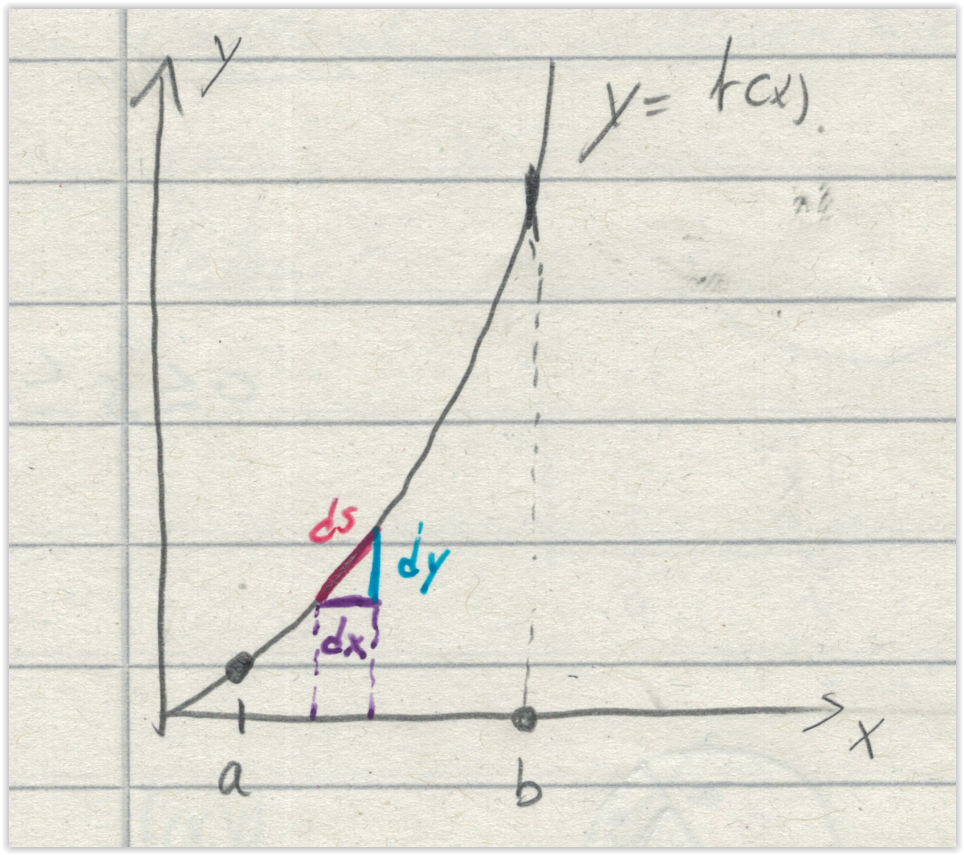
\includegraphics[width=0.4\linewidth]{./img/kurvenlaenge.png}
			  \caption{Kurvenlänge}
			  \label{fig:lkurvenlaenge}
      \end{figure}
	  \end{bem}
	  
	  \subsubsection{Flächen geschlossener ebener Kurven}
	  \begin{equation}
	    F(c) = \frac{1}{2} \int\limits_a^b \big|\big(x(t)\dot{y}(t) - y(t)\dot{x}(t)\big)\big|dt
	  \end{equation}
  \subsection{Wegintegrale}
	  \subsubsection{Wegintegral erster Art}
	  \begin{definition}
	    Das Wegintegral erster Art ist definiert durch:
	    \begin{equation}
	      \int\limits_c \varrho \; dx = \int\limits_x \varrho \; ds = \int\limits_a^b \varrho(c(t)) \quad || \dot{c}(t)|| dt \label{eq:wegintegral_1}
	    \end{equation}
	  \end{definition}
	  \begin{bem}
	    Aus \eqref{fig:wegintegral_erster_2} geht
	    \begin{equation*}
	      ds = \sqrt{dx^2 + dy^2}
	    \end{equation*}
	    hervor. Damit folgt:
	    \begin{align*}
	      ds &= \sqrt{dx^2 + dy^2} = \frac{dt}{dt}  \sqrt{dx^2 + dy^2} = \frac{1}{dt} \sqrt{dx^2 + dy^2}dt \\
	      &=  \sqrt{\frac{1}{dt^2}(dx^2 + dy^2)} =  \sqrt{\left(\frac{dx}{dt}\right)^2 + \left(\frac{dy}{dt}\right)^2}
	    \end{align*}
	    Überträgt man das bekannte Integral aus dem $\R^2$, das mit $\int\limits_a^b f(x) dx$ gegeben ist, und  obigen Zusammenhang ein, so erhält man:
	    \begin{align*}
	      \int\limits_{t=a}^{t=b} f(x,y) ds = \int\limits_{t=a}^{t=b} f(x,y) \sqrt{dx^2 + dy^2}\\
	      = \int\limits_{t=a}^{t=b} \underbrace{f(x(t),y(t))}_{\text{Höhe}} \underbrace{\sqrt{\left(\frac{dx}{dt}\right)^2 + \left(\frac{dy}{dt}\right))^2} dt}_{ds}
	    \end{align*}
	  \end{bem}
	  \begin{figure}[H] 
		\centering
		\begin{minipage}{.5\textwidth}
		  \centering
		  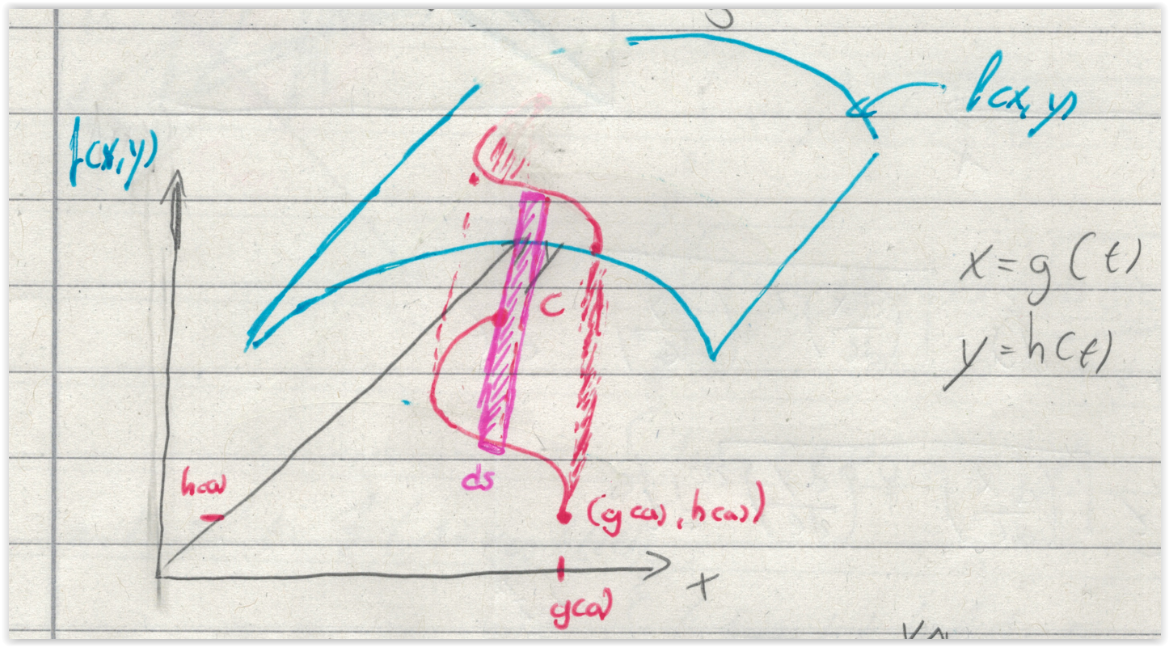
\includegraphics[width=0.9\linewidth]{./img/wegintegral_erster_1.png}
		  \caption{Graphische Interpretation}
		  \label{fig:wegintegral_erster_1}
		\end{minipage}%
		\begin{minipage}{.5\textwidth}
		  \centering
		  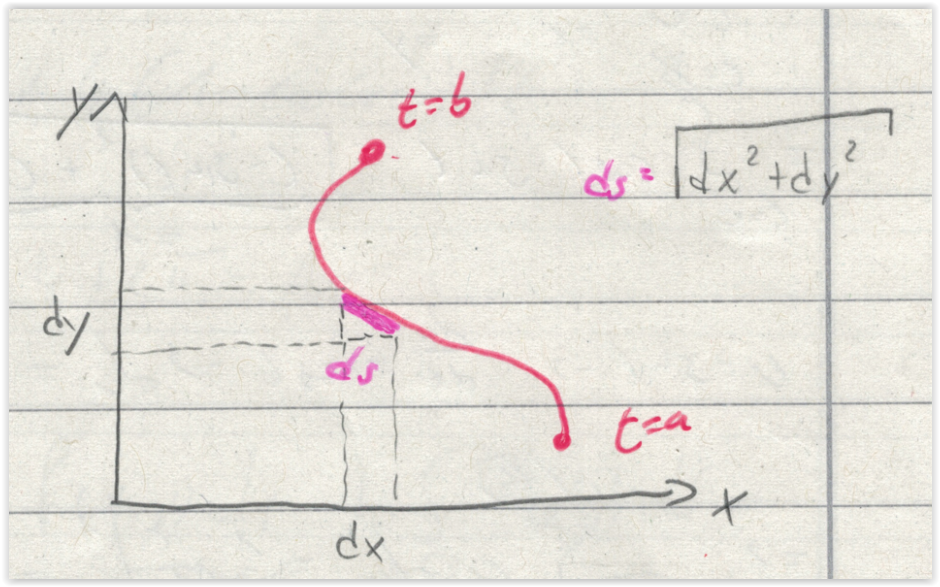
\includegraphics[width=0.8\linewidth]{./img/wegintegral_erster_2.png}
		  \caption{Interpretation von \protect\eqref{eq:wegintegral_1}}
		  \label{fig:wegintegral_erster_2}
		\end{minipage}
		\end{figure}
		\begin{bem}
			\begin{itemize}
			  \item[a) ] Integrale sind unabhängig von der gewählten Parametrisierung.
			  \item[b) ] Falls $c$ geschlossen ist so schreibt man 
				  \begin{equation}
				    \oint\limits_c \varrho \; ds
				  \end{equation}
			\end{itemize}
		\end{bem}
		\subsubsection{Wegintegrale zweiter Art}
		\begin{definition}
		  Sei $f: D\rightarrow \R^d$ ein stetiges Vektorfreld mit $D\subset \R^d$ und sei $c:[a,b] \rightarrow D$ eine stückweise $C^1$-Kurve, dann heißt 
		  \begin{equation}
		    \int\limits_c <f(x), dx> = \int\limits_a^b <f\left(c(t)\right), \dot{c}(t)>dt
		  \end{equation}
		  das Wegintegral 2-ter Art. Falls $c$ geschlossen ist schreibt man
		  \begin{equation}
		    \oint\limits_c <f(x), dx>
		  \end{equation}
		\end{definition}
		\begin{bem}
		  Das Wegintegral ist unabhängig von der gewählten Parametrisierung.
		\end{bem}
		\begin{bem}
		  Eine Alternative ältere Schreibweise ist
		  \begin{equation*}
		    \int\limits_c <f(X),dX>
		  \end{equation*}
		  Achtung, es handelt sich nur um eine Schreibweise. Nicht das Skalarprodukt aus $f(X)$ und $dX$ bilden!
		\end{bem}
		\begin{definition}
  		Ein stetiges Vektorfeld $f$ heißt wirbelfrei, falls die Kurvenintegrale längs aller stückweise stetig diffbaren Kurven verschwinden, d.h.
  		\begin{equation}
  		  \oint\limits_c <f(x), dx> = 0
  		\end{equation}
  		gilt.
		\end{definition}
		Als Konsequenz daraus folgt die Wegunabhängigkeit der Kurvenintegrale für den Fall das $f$ wirbelfrei ist. Das heißt, ist $f$ wirbelfrei, so gilt:
		\begin{equation}
		  \int\limits_{c_1} <f(x),dx> = \int\limits_{c_2} <f(x),dx>
		\end{equation}
		für beliebige Wege $c_1$ und $c_2$ mit gleichen Anfangs- und Endpunkten.
		\begin{definition}
		  Eine Teilmenge $D \subset \R^d$ heißt (weg)-zusammenhängend, falls je zwei Punkte $x,y \in D$ durch eine stückweise $C^1$-Kurve in $D$ verbunden werden können.
		  \begin{figure}[H] 
			  \centering
			  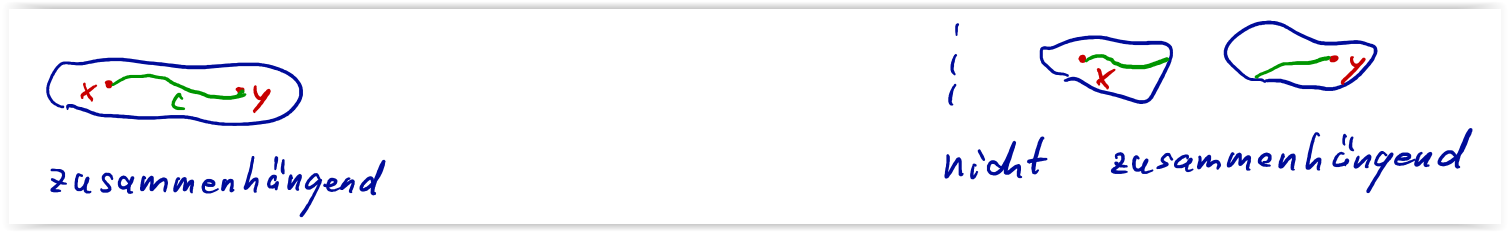
\includegraphics[width=0.8\linewidth]{./img/zusammenhaengend.png}
			  \caption{Visualisierung zusammenhängend \protect\cite{HM12}}
			  \label{fig:zusammenhängend}
		  \end{figure}
		\end{definition}
		\subsubsection{Potential}
	  \begin{definition}
	    Sei $f:D\rightarrow \R^d$ ein Vektorfeld auf $D\subset \R^d$. Wir sagen $f$ ist ein gradientenfeld, falls es eine skalare $C^1$-Funktion $\varphi: D\rightarrow\R$ gibt, mit 
	    \begin{equation}
	    \nabla \varphi(x) = f(x)
	    \end{equation}
	    $\varphi$ heißt das Potential von $f$.
	  \end{definition}
    \begin{satz}
      Sei $D \subset \R^n$ offen und zusammenhängend und $f$ ein stetiges Vektorfeld auf $D$. 
      \begin{itemize}
        \item[a) ] Besitzt $f$ ein Potential $\varphi$, so gilt für alle stückweisen $C^1$-Kurven $c$, dass 
        \begin{equation}
          \int\limits_c <f(x),dx> = \varphi(c(b)) - \varphi(c(a))
        \end{equation}
        wobei $c:[a,b]\rightarrow \R^d$. D.h. das Wegintegral ist damit wegunabhängig und $f$ wirbelfrei.
        \item[b) ] Ist $f$ wirbelfrei, so besitzt $f$ ein Potential $\varphi$ mit der Darstellung 
        \begin{equation}
          \varphi(x) = \int\limits_{c_x} f(\tilde{x}),d\tilde{x}>
        \end{equation}
        wobei $c_x$ ein Weg nach $x$ mit fest gewähltem Startpunkt $x^*$ sein soll.
      \end{itemize}
    \end{satz}	  
	  \subsubsubsection{Berechnung von Potentialen}
	  Die notwendige (aber nicht hinreichende) Bedingung für die Existenz eines Potentials ist:
	  \begin{equation}
	    rot(\nabla \varphi) = 0 \Rightarrow rot(f) = 0 \Rightarrow Potential\;ex.  
	  \end{equation}
	  \begin{definition}
	    Ein Gebiet $G$ heißt einfach zusammenhängend, falls jeder geschlossene Weg in $G$ auf einen Punkt im Gebiet zusammen gezogen werden kann.
	    \begin{figure}[H] 
			  \centering
			  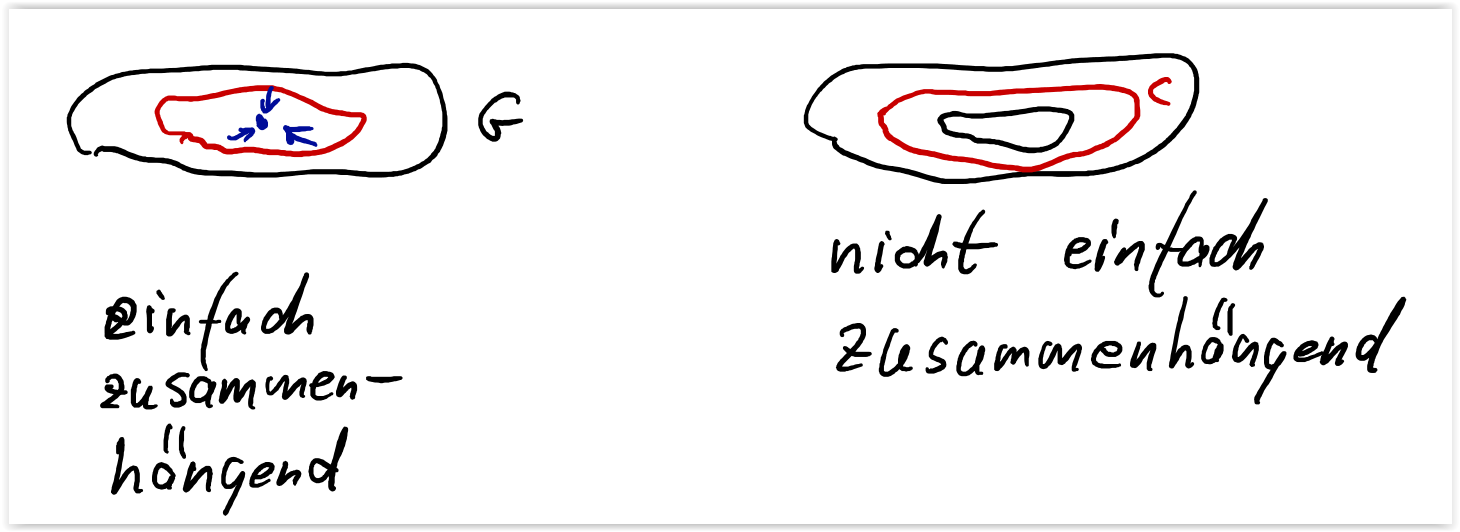
\includegraphics[width=0.8\linewidth]{./img/einfach_zusammenhaengend.png}
			  \caption{Visualisierung einfach zusammenhängend \protect\cite{HM12}}
			  \label{fig:einfach_zusammenhängend}
		  \end{figure}
	  \end{definition}
	  
  \newpage
	\section{Transformation und Koordinatensysteme}
	\subsection{Motivation}
	\textbf{Problem}:	Bisher ist war es uns nur möglich über Quader oder Normalbereiche zu integrieren. Es fehlt eine universelle Möglichkeit. \newline
	\textbf{Idee}: 1-dimensionale Substitution $\int_{x(a)}^{x(b)} f(t) \;dt = \int_a^b f(x(u))x'(u)\;du$.
	$\Rightarrow$ Es wird ein Integral über dem Intervall $(x(a), x(b))$ durch ein Integral über dem Intervall $(a,b)$ angenähert. \newline
	Ist es möglich ein Gebietsintegral über einem komplizierten Gebiet $D$ durch ein Integral über einem einfachen Gebiet $B$ darzustellen?\newline
	\textbf{Also}:
	\begin{equation}
		\int_D f(\vec{x})\;d\vec{x} = \int_B g(\vec{y})\;d\vec{y}
	\end{equation}
	Wobei $B$ idealerweise ein Normalbereich sein sollte. Wir brauchen eine Verknüpfung beider Integrale!
	\begin{equation*}
		\Rightarrow \Psi: B \to D
	\end{equation*}
	\textbf{Idee}: 1-dimensionale Substitutionsregel nutzt die Ableitung der Funktion. Funktioniert das analog im n-dimensionalen mit der Jacobi-Matrix?
	
	 \subsection{Transformation}
	 Eine Transformation bewirkt einen Wechsel des Koordinatensystems. Wir stellen folgende Bedingungen an die Transformationsabbildung:
	 \begin{description}
	 	\item[(1) ] Sie soll bijektiv sein. \\
	 	\item[(2) ] Sie soll stetig differenzierbar sein und für die Funktionaldeterminanten soll
	 	\begin{equation}
	 		\det \Psi'(\vec{x}) < 0 \text{ oder } \det \Psi'(\vec{x}) > 0
	 	\end{equation}
	 	f.f.a. $\vec{x} \in B$ gelten.
	 	\textbf{(1)} Stellt dabei sicher, dass das komplette Volumen von $B$ berücksichtigt wird und das keine Bereiche doppelt gezählt werden. \textbf{(2)} vermeidet Widersprüche durch konstruierte Funktionen die z.B. bei einer Transformation zu einer Nullmenge führen würden.
	 \end{description}
	 
	 \begin{bem}
	 	Die Funktionaldeterminante ist gegeben durch
	 	\begin{equation}
	 		\Psi' := |J(f(\vec{x}))|
	 	\end{equation}
	 \end{bem}
	 
	 Für $B,D$ und $\Psi: B \to D$ sollen die eben formulierten Vorraussetzungen gelten. Eine Funktion $f: D\to \R$ ist genau dann über $D$ integrierbar, wenn $f(\Psi(\cdot))|det \Psi'|$ über $B$ integrierbar ist und es gilt
	 \begin{equation}
	 	\int_D f(\vec{x}) \; d\vec{x} = \int_B f(\Psi(\vec{y})) |det \Psi'(\vec{y})| \; d\vec{y} = \int_B f(\vec{u}) |det J_{\vec{x}}(\vec{u})| \; dB
	 \end{equation}
	 
	 \subsubsection{Ablauf der Koordinatentransformation}\label{subs:abl_koordinatentrans}
	 Der allgemeine Ablauf einer Koordinatentransformation soll hier anhand einer Oberflächeninteration gezeigt werden.
	\begin{flalign*}
    	&\text{Angaben zum Beispiel}&
  	\end{flalign*}
  	Zu bestimmen ist der Flächeninhalt des folgenden Graphen:
  	\begin{equation}
  		f_1:\lbrace(x,y) \in \R^2| 1 \leq x^2 + y^2 \leq 4 \rbrace \to \R,\quad (x,y) \mapsto xy
  	\end{equation}
  	\begin{figure}[H] 
		  \centering
		  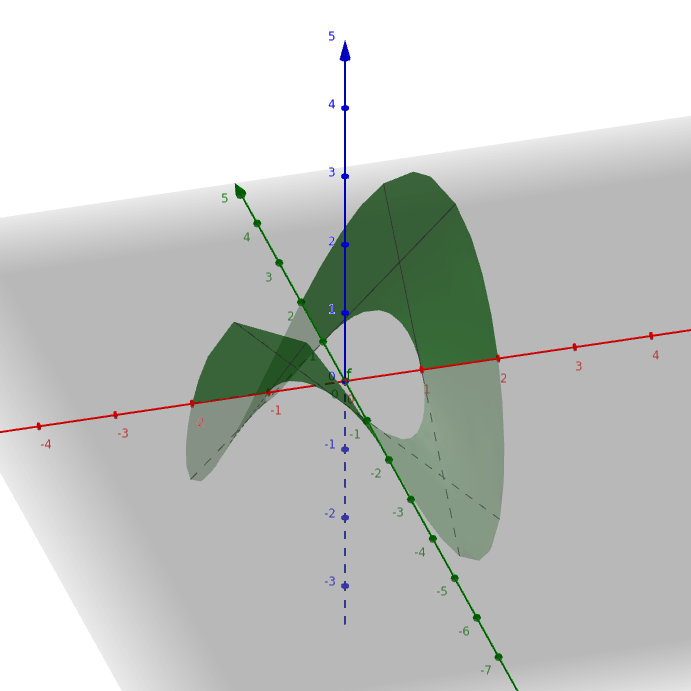
\includegraphics[width=0.5\textwidth]{./img/transf_bsp_a.png}
		  \caption{Zu untersuchendes Gebiet}
		  \label{fig:transf_bsp_a}
	  \end{figure}
	  \vspace{-1cm}
	\begin{flalign*}
    &\textbf{Schritt 1: } \text{Vektorfeld aus den Angaben schließen}&
  \end{flalign*}
    \vspace{-0.5cm}
    \begin{align}
    	v\vec{v} = \vecT{x \\ y \\xy}
    \end{align}
      \vspace{-0.5cm}
  \begin{flalign*}
    &\textbf{Schritt 2: } \text{Allgemeines Oberflächenintegral aufstellen und vereinfachen}&
  \end{flalign*}
    \vspace{-0.5cm}
  \begin{align*}
    O_F(f_1)  &= \int_F \;d\sigma = \int_B \left| \left| \frac{\partial \vec{v}}{\partial x} \times \frac{\partial \vec{v}}{\partial y} \right| \right| \; d(x,y) \\
    &= \int_B \sqrt{y^2 + x^2 + 1} \;d(x,y)
  \end{align*}
    \vspace{-0.5cm}
  \begin{flalign*}
    &\textbf{Schritt 3: } \text{Parametrisierung auf die transformiert werden soll aufstellen (hier Polarkoordinaten)}&
  \end{flalign*}
    \vspace{-0.5cm}
  \begin{align*}
  	\gamma = \vecT{r \cdot \cos \varphi \\ r \cdot \sin \varphi} \quad, 1 \leq r \leq 2,\; 0 \leq \varphi \leq 2\pi
  \end{align*}
  Wobei zu beachten ist, dass $\gamma_1$ analog zu $\gamma$ parametrisiert ist. Einzig geändert hat sich die obere Schranke für $r$ wie unschwer an den Integralsgrenzen zu erkennen ist.
  \begin{flalign*}
    &\textbf{Schritt 4: } \text{Verzerrungsfaktor berechnen}&
  \end{flalign*}	
	 \vspace{-0.5cm}
  \begin{align*}
  	\left| \det J_{\gamma}(r,\varphi)\right| = \left| 
  	\begin{array}{c c}
  		\cos \varphi & -r \sin \varphi \\
  		\sin \varphi & r \cos \varphi
	\end{array}  	  \right| = r
  \end{align*}
  \vspace{-0.5cm}
	 \begin{flalign*}
    &\textbf{Schritt 5: } \text{Transformationsparametrisierung und Verzerrungsfaktor einsetzen}&
  \end{flalign*}	
	 \vspace{-0.5cm}
  \begin{align*}
  O_F(f_1) &= \int_0^{2\pi} \int_1^2 \sqrt{r^2 + 1} r \; dr d\varphi \quad, \text{ mit }u:= 1+r^2 \Rightarrow du= 2r \;dr \text{ folgt} \\
  &= \frac{1}{2} \int_0^{2\pi} \int_{1+1^2}^{1+2^2} \sqrt{u} \;du d\varphi = \frac{1}{2} \int_0^{2\pi} \frac{2}{3} u^{\frac{3}{2}}\Big|_2^5 \; d\varphi = \pi \frac{2}{3} \left(\sqrt{5^3} - \sqrt{2^3}\right) = \frac{2\pi}{3} \left(5 \sqrt{5} - 2\sqrt{2}\right)
  \end{align*}  
	 
	 \subsection{Wichtige Koordinatensysteme}
	 \subsubsection{Polarkoordinaten}
	 Im $\R^2$ gegeben durch eine Parametrisierung mit $(r,\varphi)$, wobei $0 \leq r$ den Abstand eines Punktes vom Ursprung und $\varphi \in (-\pi, \pi)$ den Winkel zwischen der Verbindungsstrecke des Punktes mit dem Ursprung und der positiven $x-1$-Achse bezeichnet. Die Parametrisierung ist gegeben durch;
	 \begin{align}
	 	\Psi(r,\varphi) = \vecT{  r\cdot \cos \varphi \\ r \cdot \sin \varphi} \qquad, (r,\varphi) \in B \\
	 	\text{mit } 0\leq \text{ und } -\pi \leq \varphi \leq \pi \text{ oder } 0 \leq \varphi \leq 2\pi \nonumber 
	 \end{align}
	 damit ergibt sich
	 \begin{align}
	 J_{\Psi}(r, \varphi) &= \left(
	 	\begin{array}{c c}
	 		\cos \varphi & -r \sin \varphi \\
	 		\sin \varphi & r \cos \varphi
	 	\end{array}  \right) \\
	 	\Rightarrow \Psi'(r,\varphi) &= r \cos^2 \varphi + r \sin^2 \varphi = r
	 \end{align}
	 Ist $D \subset \R^2$, $f \in L(D)$ und $B$ die Beschreibung von $D$ durch Polarkoordinaten, so gilt
	 \begin{equation}
	 	\int_D f(x_1,x_2) \; d(x_1,x_2) = \int_B f(r \cos \varphi, r \sin \varphi) r \; d(r,\varphi)
	 \end{equation}
	 
	 \subsubsection{Zylinderkoordinaten}
	 Zylinderkoordinaten erweitern Polarkoordinaten um eine dritte Dimension. Es wird praktisch einfach eine dritte Koordinate angefügt. Damit ergibt sich für die Parametrisierung
	 \begin{align}
	 	\Psi(r,\varphi,z) &= \vecT{r\cdot \cos \varphi \\ r \cdot \sin \varphi \\ z} \\
	 	\text{mit } (r,\varphi,z) \in B \text{, } 0\leq r &\text{ und } -\pi \leq \varphi \leq pi \text{ oder } 0 \leq \varphi \leq 2\pi \nonumber
	 \end{align}
	 Damit ergibt sich 
	 \begin{align}
	 	J_{\Psi} (r,\varphi,z) &= \left(
	 	\begin{array}{c c c}
	 		\cos \varphi & -r \sin \varphi & 0 \\
	 		\sin \varphi & r \cos \varphi & 0 \\
	 		0 & 0 & 1	 	
	 	\end{array} \right) \\
	 	&\Rightarrow \Psi'(r,\varphi,z) = r
	 \end{align}
	 Ist $D \subset \R^3$, $f \in L(D)$ und $B$ die Beschreibung von $D$ durch Zylinderkoordinaten, so gilt
	 \begin{equation}
	 	\int_D f(x_1,x_2,x_3) \; d(x_1,x_2,x_3) = \int_B f(r \cos \varphi, r \sin \varphi,z) r \; d(r,\varphi,z)
	 \end{equation}
	 
	 \subsubsection{Kugelkoordinaten}
	 Man überträgt die Idee der Darstellung durch einen Abstand $r$ und Winkel $\varphi$ wie aus den Polarkoordinaten bekannt auf den $\R^3$. Zusätzlich variiert man einen Winkel um die $z$-Koordinate herum. So ergibt sich die Parametrisierung zu:
	 \begin{align}
	 	\Psi (r,\varphi,\vartheta) = \vecT{r \cos \varphi \sin \vartheta \\ r \sin \varphi \sin \vartheta \\ r \cos \vartheta} \\
	 	\text{mit } 0 \leq r ,\; -\pi \leq \varphi \leq \pi, \; 0 \leq \vartheta \leq \pi \nonumber
	 \end{align}
	 Damit ergibt sich
	 \begin{align}
	 	J_{\Psi}(r, \varphi, \vartheta) &= \left(
	 	\begin{array}{c c c}
	 		\cos \varphi \sin \vartheta & -r \sin \varphi \sin \vartheta & r \cos \varphi \cos \vartheta \\
	 		sin \varphi \sin \vartheta & r \cos \varphi \cos \vartheta & r \sin \varphi \cos \vartheta \\
	 		\cos \vartheta & 0 & -r \sin \vartheta
	 	\end{array} \right) \\
	 	&\Rightarrow \Psi'(r,\varphi, \vartheta) = -r^2 \sin \vartheta
	 \end{align}
	 Ist $D \subset \R^3$, $f \in L(D)$ und $B$ die Beschreibung von $D$ durch Kugelkoordinaten, so gilt
	 \begin{align}
	 	\int_D f(x_1,x_2,x_3) \;&d(x1,x2,x3) \nonumber \\
	 	&= \int_b f(r \cos \varphi \sin \vartheta, r \sin \varphi \sin \vartheta, r \cos \vartheta) \cdot r^2 \sin \vartheta \;d(r,\varphi, \vartheta)
	 \end{align}
	
	\section{DGL 2. Ordnung}
	\subsection{Allgemeines zu DGL 2. Ordnung mit konstanten Koeffizienten}
	Wir betrachten lineare DGL 
	\begin{equation}
		Ly := y'' + ay' + by = f(x) \label{eq:dgl_ordnZwei_allg}
	\end{equation}
	mit $a,b \in \R$ und Anfangsbedingungen der Form
	\begin{equation}
		y(x_0) = y_0,\quad y'(x_0) = v_0
	\end{equation}
	
	\begin{satz}
		Ist $f$ stetig auf einem Intervalll $I \in \R$, dann hat jedes AWP genau eine Lösung  die auf ganz $I$ existiert.
	\end{satz}
	
	\begin{satz}
		Superpositionsprinzip: \newline
		Sind $y_1,y_2$ $C^2$-Funktionen mit 
		\begin{align*}
			Ly_1 = f_1 \\
			Ly_2 = f_2
		\end{align*}
		dann gilt für alle $C_1,C_2 \in \R$ und $y = C_1 y_1 + C_2 y_2$
		\begin{equation}
			Ly = C_1 f_1 + C_2 f_2
		\end{equation}
		wobei
		\begin{align*}
			y(0) = C_1 y_1 (0) + C_2 y_2 (0) \\
			y'(0) = C_1 y_1' (0) + C_2 y_2' (0)
		\end{align*}
		\textbf{Folgerung}: Die Menge $\mathcal{L}$ der Lösungen der homogenen Gleichung 
		\begin{equation}
			Ly = 0 \label{eq:dgl_supPos_b}
		\end{equation}
		ist ein Vektorraum über $\R$. Jede Basis von $\mathcal{L}$ heißt Fundamentalsystem von \eqref{eq:dgl_supPos_b}.
	\end{satz}
	
	\begin{satz}
		Der Raum $\mathcal{L}$ der Lösungen von \eqref{eq:dgl_supPos_b} ist zweidimensional. Sind $y_1,y_2 \in \mathcal{L}$ linear unabhängig, dann gilt
		\begin{equation}
			\mathcal{L} = \lbrace C_1 x_1 + C_2 y_2 | C_1,C_2 \in \R \rbrace
		\end{equation}
	\end{satz}
	
	\begin{bem}
		Zwei Funktionen heißen linear unabhängig, wenn
		\begin{equation}
			C_1 y_1 + C_2 y_2 = 0 \Rightarrow C_1 = 0, C_2 = 0
		\end{equation}
	\end{bem}
	
	\begin{satz}
		ist $\lbrace y_1, y_2 \rbrace$ ein Fundamentalsystem von \eqref{eq:dgl_supPos_b}, und $y_p$ eine partikuläre Lösung von \eqref{eq:dgl_ordnZwei_allg}, dann ist
		\begin{equation}
			y = y_p + C_1 y_1 + C_2 y_2 \qquad, C_1,C_2 \in \R
		\end{equation}		 
		die vollständige Lösung von \eqref{eq:dgl_ordnZwei_allg}.
	\end{satz}
	
	\subsection{Ansätze (Erinnerung an HM1)}
	\begin{definition}
    Lineare skalare Diff.gleichungen mit konst. Koeffizienten sind Gleichungen der bauart:
    \begin{align*}
      Ly(x) = a_n y^{(n)}(x)+a_{n-1}y^{(n-1)}(x)+...+a_1y'(x) + a_o y(x) = f(x)
    \end{align*}
  \end{definition}
  \subsubsection{Ansätze}
  \begin{itemize}
    \item[a)] Homogene Diff.gleichung:
    Mit $\lambda$ als einfache NST:
    \begin{equation}
      y(x) = e^{\displaystyle\lambda x} \label{eq:dgl_Ansatz_a}
    \end{equation}
    Mit $\lambda$ als $n$-fache NST:
    \begin{equation}
      f(x) = e^{\displaystyle\lambda x}, xe^{\displaystyle\lambda x}, ..., x^{n-1}e^{\displaystyle\lambda x} 
    \end{equation}
    Mit $\lambda = \alpha + \beta i$ (komplexe Nullstellen):
    \begin{equation}
      e^{\alpha x}cos(\beta x),\quad e^{\alpha x} sin(\beta x)
    \end{equation}
    \item[b)] Inhomogenität der Form $f(x) = p_k(x) e^{sx}$ mit $p_k(x)$ als ein Polynom $k$-ten Grades.
    \begin{equation}
      y_p(x) = R_k(x)e^{sx}x^q
    \end{equation}
    Mit $R_k(x) = a_kx^k+...+a_0$ und $q$ als Vielfachheit der Nullstelle $s$ (ist $s$ keine Nullstelle so ist $q = 0$ und damit $x^q = 1$).
    \item[c)] Inhomogenität der Form $cos(kx)$ oder $sin(kx)$.
    \begin{equation}
      yp(x) = (a cos(kx) + b sin(kx)) x^q
    \end{equation}
    Beispiel Umformung:
    \begin{align}
      f(x) &= sin(4x)\nonumber\\
      Mit \quad
      (1)\;\;\; e^{i\varphi} &= cos \varphi + i sin\varphi\nonumber \\
      und \quad
      (2)\; e^{-i\varphi} &= cos \varphi - i sin \varphi\nonumber\\
      folgt \;mit \;(1) + (2) \;&bzw.\; (1)-(2)\nonumber\\
      e^{i\varphi} + e^{-i\varphi} = 2\;cos\varphi \quad &bzw. \quad e^{i\varphi}-e^{-i\varphi} = 2 \; sin\varphi\nonumber\\
      \Rightarrow cos \varphi = \frac{1}{2} (e^{i\varphi}+e^{-i\varphi}) &\quad \Rightarrow sin \varphi = \frac{1}{2i} (e^{i\varphi}-e^{-i\varphi}),\quad \forall \varphi \in \R
    \end{align}
    $q$ im Ansatz gibt die Vielfachheit der NST $i \varphi$ im charackteristischen Polynom des homogenen Teils der Gleichung an.
    \item[d)] Inhomogenität der Form $q_k(x)e^{\alpha x} cos(\beta x)$ oder $q_k(x)e^{\alpha x} sin(\beta x)$
    \begin{equation}
      yp(x) = R_k(x)x^qe^{\alpha x}cos(\beta x) + \tilde{R}_k(x) x^qe^{\alpha x}cos{\beta x}
    \end{equation}
  \end{itemize}
  \subsubsection{Vorgehensweise}
    \begin{flalign*}
      &\textbf{Schritt 1: } \text{Ansatz wählen}&
    \end{flalign*}
      \vspace{-0.5cm}
    \begin{flalign*}
      &\textbf{Schritt 2: } \text{Ansatz einsetzen und charackteristisches Polynom bilden}& \\
      &\text{Beispiel:}&
    \end{flalign*}
      \vspace{-1cm}
    \begin{align*}
      &y'' + 3y'+2y = 0 \\
      &\overset{\eqref{eq:dgl_Ansatz_a}}{\Rightarrow} \left(e^{\lambda x}\right)'' + 3\left(e^{\lambda x}\right)' + 2e^{\lambda x} = 0 \\
      \left(e^{\lambda x}\right)' &\;\;= \lambda e^{\lambda x} \Rightarrow \left(e^{\lambda x}\right)'' = \lambda^2 e^{\lambda x} \\
      &\;\;\Rightarrow \lambda^2 + 3 \lambda + 2 = 0
    \end{align*}
      \vspace{-0.5cm}
    \begin{flalign*}
      &\textbf{Schritt 3.1: } \text{Nullstellen des char. Polynoms suchen und in Ansatz einsetzen}&\\
      &Beispiel:&
    \end{flalign*}
      \vspace{-0.5cm}
    \begin{align*}
      \lambda^2 + 3 \lambda + 2 = 0 \Rightarrow \lambda_1 = -2,\quad \lambda_2 = -1
    \end{align*}
      \vspace{-0.5cm}
    \begin{flalign*}
      &\textbf{Schritt 3.2: } \text{Gegebenenfalls komplexe NST in reale umwandeln}&\\
      &Beispiel:&
    \end{flalign*}
      \vspace{-1cm}
    \begin{align*}
      y(x) &= C_1 e^{-x+ix} + C_2 e^{-x-ix} \\
      \Rightarrow y(x) &= \tilde{C}_1e^{-x}cosx + \tilde{C}_2 e^{-x}sinx \qquad, \tilde{C}_1, \tilde{C}_2 \in \R
    \end{align*}
      \vspace{-0.5cm}
    \begin{flalign*}
      &\textbf{Schritt 4: } \text{Allgemeine Lösung aufstellen}&
    \end{flalign*}
      \vspace{-0.5cm}
    \begin{align*}
      \Rightarrow y(x) = C_1 e^{-2x} + C_2 e^{-x}\quad, C_1,C_2\in \R
    \end{align*}

    \subsubsubsection{Anfangswertproblem}
    Falls Anfangswerte vorhanden sind können an dieser Stelle die Konstanten Koeffizienten explizit bestimmt werden. \newline
    \begin{flalign*}
    &Beispiel:&
    \end{flalign*}
      \vspace{-1cm}
    \begin{align*}
	    y(0) &= 1,\;y'(0) = 0\\
	    y(t) &= C_1 e^{5t} + C_2 e^{-2t}\\
	    &\Rightarrow y(0) = C_1 e^{5\cdot 0} + C_2 e^{-2\cdot 0} = 1\\ 
      &\Rightarrow C_1 = 1-C_2\\
      y'(t)& = 5 C_1 e^{5t} -2 C_2 e^{-2t} \Rightarrow y'(0) = 5C_1 - 2C_2 = 0\\
      &\Rightarrow y'(0) = 0 = 5(1-C_2)-2C_2 \Rightarrow C_2 = \frac{5}{7}\\
      &\Rightarrow C_1 = 1-C_2 = 1- \frac{5}{7} = \frac{2}{7}\\
      \; \\
      &\Rightarrow y(t) = \frac{2}{7} e^{5t}+\frac{5}{7}e^{-2t}
    \end{align*}
    
    \subsubsubsection{Inhomogenität}
      \begin{flalign*}
        &\textbf{Schritt 1: } \text{Ansatz wählen}&
      \end{flalign*}
      \vspace{-0.5cm}
      \begin{flalign*}
        &\textbf{Schritt 2: } \text{Ansatz gegebenenfalls ableiten und in homogenen Teil einsetzen}&
      \end{flalign*}    
      \vspace{-0.5cm}
      \begin{flalign*}
        &\textbf{Schritt 3: } \text{Über Koeffizientenvergleich Vorfaktoren bestimmen}&
      \end{flalign*}    
      \vspace{-0.5cm}
      \begin{flalign*}
        &\textbf{Schritt 4: } \text{Allgemeine Lösung bilden}&
      \end{flalign*}    
      \vspace{-0.5cm}
      \begin{equation}
        y(x) = y_{hom}(x) + y_p(x)
      \end{equation}
      \vspace{-0.5cm}
      \begin{flalign*}
        &\textbf{Schritt 5: } \text{Gegebenenfalls Anfangswertproblem lösen}&
      \end{flalign*}    
	\section{Integralsätze}
	Integralsätze bilden Zusammenhänge zwischen Kurven-, Oberflächen- und Volumenintegralen. \newline
	\textbf{Analogie 1-d}: Der Hauptsatz der Differential- und Integralrechnung im eindimensionalen
	\begin{equation}
		\int_a^b f(x) \dx = F(b) - F(a)
	\end{equation}
	$\Rightarrow$ Das Integral über eine Funktion $f$ lässt sich bestimmen, wenn man die Werte einer verwandten Funktion $F$ an den Randpunkten kennt.
	\textbf{Übertragung aufs n-d}: Bestimmte Integrale über $\vec{v}$ lassen sich ermitteln, wenn die Werte eines verwandten Vektors $\vec{w}$ am Rand bekannt sind. Der Rand einer Fläche oder eines Volumens ist aber ausgedehnt, also muss auch hier integriert werden.
	
	\begin{bem}
		Hier kann nun eine alternative Interpretation für den Begriff Integralsatz getroffen werden - Ein Integralsatz ist eine Beziehung, die eine Verbindung zwischen dem Integral über ein Objekt und dessen Rand herstelllt.
	\end{bem}
	
	\subsection{Kurvenintegrale (Erinnerung HM2)}
	
	\subsubsection{Wegintegral erster Art}
	  \begin{definition}
	    Das Wegintegral erster Art ist definiert durch:
	    \begin{equation}
	      \int\limits_c \varrho \; dx = \int\limits_x \varrho \; ds = \int\limits_a^b \varrho(c(t)) \quad || \dot{c}(t)|| dt \label{eq:wegintegral_1}
	    \end{equation}
	  \end{definition}
	  \begin{bem}
	    Aus \eqref{fig:wegintegral_erster_2} geht
	    \begin{equation*}
	      ds = \sqrt{dx^2 + dy^2}
	    \end{equation*}
	    hervor. Damit folgt:
	    \begin{align*}
	      ds &= \sqrt{dx^2 + dy^2} = \frac{dt}{dt}  \sqrt{dx^2 + dy^2} = \frac{1}{dt} \sqrt{dx^2 + dy^2}dt \\
	      &=  \sqrt{\frac{1}{dt^2}(dx^2 + dy^2)} =  \sqrt{\left(\frac{dx}{dt}\right)^2 + \left(\frac{dy}{dt}\right)^2}
	    \end{align*}
	    Überträgt man das bekannte Integral aus dem $\R^2$, das mit $\int\limits_a^b f(x) dx$ gegeben ist, und  obigen Zusammenhang ein, so erhält man:
	    \begin{align*}
	      \int\limits_{t=a}^{t=b} f(x,y) ds = \int\limits_{t=a}^{t=b} f(x,y) \sqrt{dx^2 + dy^2}\\
	      = \int\limits_{t=a}^{t=b} \underbrace{f(x(t),y(t))}_{\text{Höhe}} \underbrace{\sqrt{\left(\frac{dx}{dt}\right)^2 + \left(\frac{dy}{dt}\right)^2} dt}_{ds}
	    \end{align*}
	  \end{bem}
	  \begin{figure}[H] 
		\centering
		\begin{minipage}{.5\textwidth}
		  \centering
		  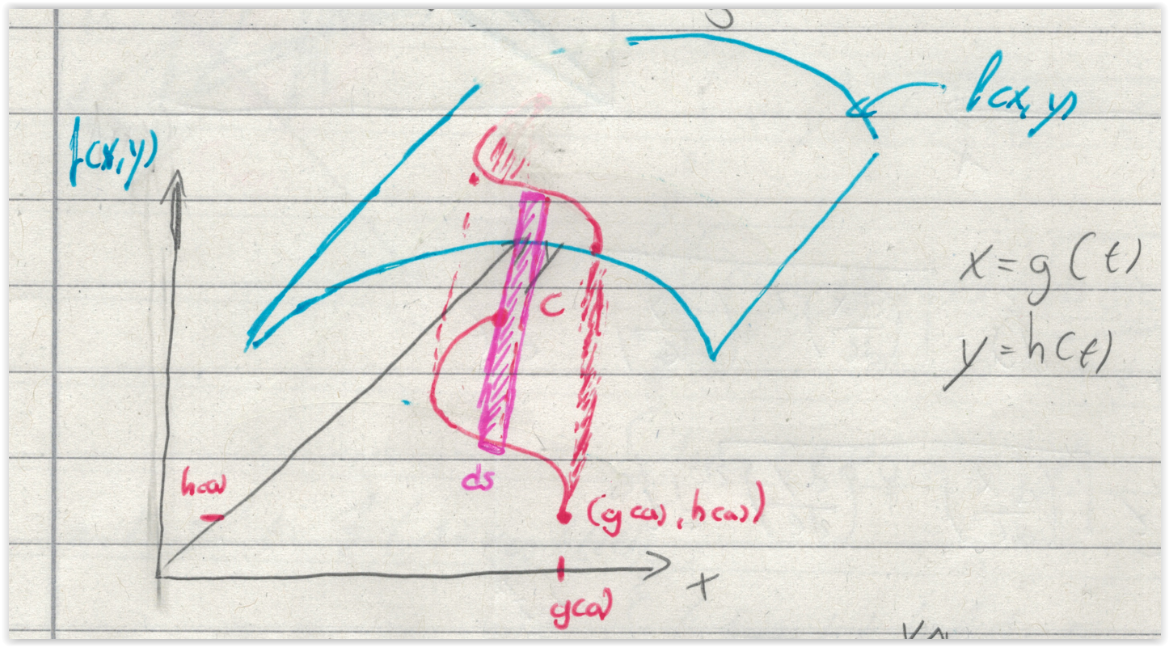
\includegraphics[width=0.9\linewidth]{./img/wegintegral_erster_1.png}
		  \caption{Graphische Interpretation}
		  \label{fig:wegintegral_erster_1}
		\end{minipage}%
		\begin{minipage}{.5\textwidth}
		  \centering
		  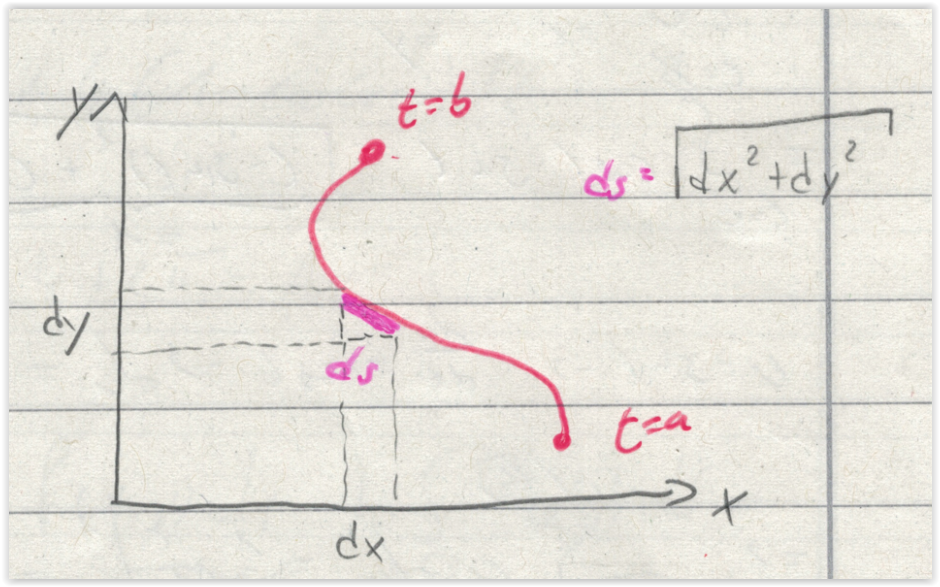
\includegraphics[width=0.8\linewidth]{./img/wegintegral_erster_2.png}
		  \caption{Interpretation von \protect\eqref{eq:wegintegral_1}}
		  \label{fig:wegintegral_erster_2}
		\end{minipage}
		\end{figure}
		\begin{bem}
			\begin{itemize}
			  \item[a) ] Integrale sind unabhängig von der gewählten Parametrisierung.
			  \item[b) ] Falls $c$ geschlossen ist so schreibt man 
				  \begin{equation}
				    \oint\limits_c \varrho \; ds
				  \end{equation}
			\end{itemize}
		\end{bem}
		\subsubsection{Wegintegrale zweiter Art}
		\begin{definition}
		  Sei $f: D\rightarrow \R^d$ ein stetiges Vektorfeld mit $D\subset \R^d$ und sei $c:[a,b] \rightarrow D$ eine stückweise $C^1$-Kurve, dann heißt 
		  \begin{equation}
		    \int\limits_c <f(x), dx> = \int\limits_a^b <f\left(c(t)\right), \dot{c}(t)>dt
		  \end{equation}
		  das Wegintegral 2-ter Art. Falls $c$ geschlossen ist schreibt man
		  \begin{equation}
		    \oint\limits_c <f(x), dx>
		  \end{equation}
		\end{definition}
		\begin{bem}
		  Das Wegintegral ist unabhängig von der gewählten Parametrisierung.
		\end{bem}
		\begin{bem}
		  Eine Alternative ältere Schreibweise ist
		  \begin{equation*}
		    \int\limits_c <f(X),dX>
		  \end{equation*}
		  Achtung, es handelt sich nur um eine Schreibweise. Nicht das Skalarprodukt aus $f(X)$ und $dX$ bilden!
		\end{bem}
		\begin{definition}
  		Ein stetiges Vektorfeld $f$ heißt wirbelfrei, falls die Kurvenintegrale längs aller stückweise stetig diffbaren Kurven verschwinden, d.h.
  		\begin{equation}
  		  \oint\limits_c <f(x), dx> = 0
  		\end{equation}
  		gilt.
		\end{definition}
		Als Konsequenz daraus folgt die Wegunabhängigkeit der Kurvenintegrale für den Fall das $f$ wirbelfrei ist. Das heißt, ist $f$ wirbelfrei, so gilt:
		\begin{equation}
		  \int\limits_{c_1} <f(x),dx> = \int\limits_{c_2} <f(x),dx>
		\end{equation}
		für beliebige Wege $c_1$ und $c_2$ mit gleichen Anfangs- und Endpunkten.
		\begin{definition}
		  Eine Teilmenge $D \subset \R^d$ heißt (weg)-zusammenhängend, falls je zwei Punkte $x,y \in D$ durch eine stückweise $C^1$-Kurve in $D$ verbunden werden können.
		  \begin{figure}[H] 
			  \centering
			  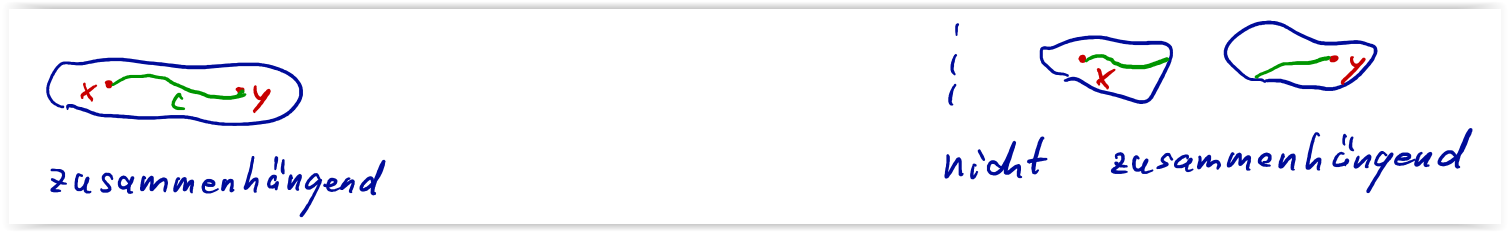
\includegraphics[width=0.8\linewidth]{./img/zusammenhaengend.png}
			  \caption{Visualisierung zusammenhängend \protect\cite{HM12}}
			  \label{fig:zusammenhängend}
		  \end{figure}
		\end{definition}
		\subsubsection{Potential}
	  \begin{definition}
	    Sei $f:D\rightarrow \R^d$ ein Vektorfeld auf $D\subset \R^d$. Wir sagen $f$ ist ein gradientenfeld, falls es eine skalare $C^1$-Funktion $\varphi: D\rightarrow\R$ gibt, mit 
	    \begin{equation}
	    \nabla \varphi(x) = f(x)
	    \end{equation}
	    $\varphi$ heißt das Potential von $f$.
	  \end{definition}
    \begin{satz}
      Sei $D \subset \R^n$ offen und zusammenhängend und $f$ ein stetiges Vektorfeld auf $D$. 
      \begin{itemize}
        \item[a) ] Besitzt $f$ ein Potential $\varphi$, so gilt für alle stückweisen $C^1$-Kurven $c$, dass 
        \begin{equation}
          \int\limits_c <f(x),dx> = \varphi(c(b)) - \varphi(c(a))
        \end{equation}
        wobei $c:[a,b]\rightarrow \R^d$. D.h. das Wegintegral ist damit wegunabhängig und $f$ wirbelfrei.
        \item[b) ] Ist $f$ wirbelfrei, so besitzt $f$ ein Potential $\varphi$ mit der Darstellung 
        \begin{equation}
          \varphi(x) = \int\limits_{c_x} <f(\tilde{x}),d\tilde{x}>
        \end{equation}
        wobei $c_x$ ein Weg nach $x$ mit fest gewähltem Startpunkt $x^*$ sein soll.
      \end{itemize}
    \end{satz}	  
	  \subsubsubsection{Berechnung von Potentialen}
	  Die notwendige (aber nicht hinreichende) Bedingung für die Existenz eines Potentials ist:
	  \begin{equation}
	    rot(\nabla \varphi) = 0 \Rightarrow rot(f) = 0 \Rightarrow Potential\;ex.  
	  \end{equation}
	  \begin{definition}
	    Ein Gebiet $G$ heißt einfach zusammenhängend, falls jeder geschlossene Weg in $G$ auf einen Punkt im Gebiet zusammen gezogen werden kann.
	    \begin{figure}[H] 
			  \centering
			  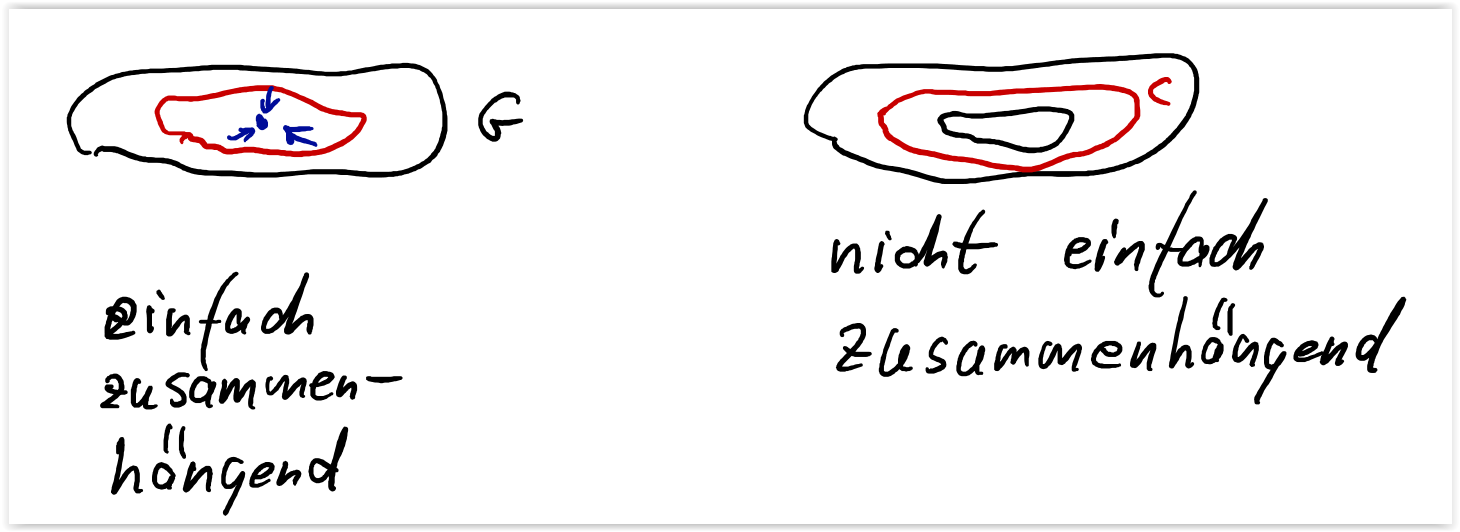
\includegraphics[width=0.8\linewidth]{./img/einfach_zusammenhaengend.png}
			  \caption{Visualisierung einfach zusammenhängend \protect\cite{HM12}}
			  \label{fig:einfach_zusammenhängend}
		  \end{figure}
	  \end{definition}
	\subsection{Definitionen}
	\subsubsection{2D-Divergenz}
	\begin{equation}
		\diverg \vec{F}(x,y) = \lim_{|A_(x,y)|\to 0} \underbrace{\frac{1}{|A_{(x,y)}|} \overbrace{\oint_c \vec{F} \vec{n}\;ds}^{\text{2d-Fluss}}}_{\text{Fluss pro Flächeneinheit}}
	\end{equation}
	\subsubsection{3D-Divergenz}
	\begin{equation}
		\diverg \vec{F}(x,y,z) = \lim_{R \to (x,y,z)}\frac{1}{|R|} \int \int_s \vec{F} \vec{n}\;ds
	\end{equation}
	\subsubsection{2D-Rotation}
	\begin{equation}
		\rot_2 \vec{F}(x,y) = \lim_{A_(x,y)\to 0} \underbrace{\frac{1}{|A_{(x,y)}|}\oint_c \vec{F} \;dr}_{\text{durchschnittliche Rotation pro Flächeneinheit}}
	\end{equation}
	\subsubsection{3D-Rotation}
	\begin{equation}
		\rot \vec{F}(x,y) \cdot \hat{e}_x = \lim_{|A_{(x,y,z)},\hat{e}_x \to 0} \frac{1}{|A_{(x,y,z)},\hat{e}|}\oint_c \vec{F} \;dr
	\end{equation}
	Analog für $\hat{e}_y$ und $\hat{e}_z$.
	
	\subsection{Satz von Green}
	Sei $f$ ein $C^1$-Vektorfeld, $D \subset \R^2$ offen und zusammenhängend. $K \subset D$ sei komplett und bezüglich beider Koordinatenrichtungen ein Normalbereich. $K$ werde von einer $C^1$-Kurve $c:t\to c(t)$ berandet. Die Parametrisierung sei  so gewählt, dass $K$ linkgs von der Durchlaufrichtung liegt. Dann gilt
	\begin{equation}
		\oint_c < \underbrace{f(\vec{x})}_{\in \R^2}, \underbrace{d\vec{x}>}_{\in \R^2} = \int_K rot_2 f(\vec{x}) \; d\vec{x}
	\end{equation}		
	Und es ist
	\begin{equation}
		\rot_2 f(\vec{x}) = \frac{\partial f_2}{\partial x_1} - \frac{\partial f_1}{\partial x_2}
	\end{equation}
	  \begin{figure}[H] 
		  \centering
		  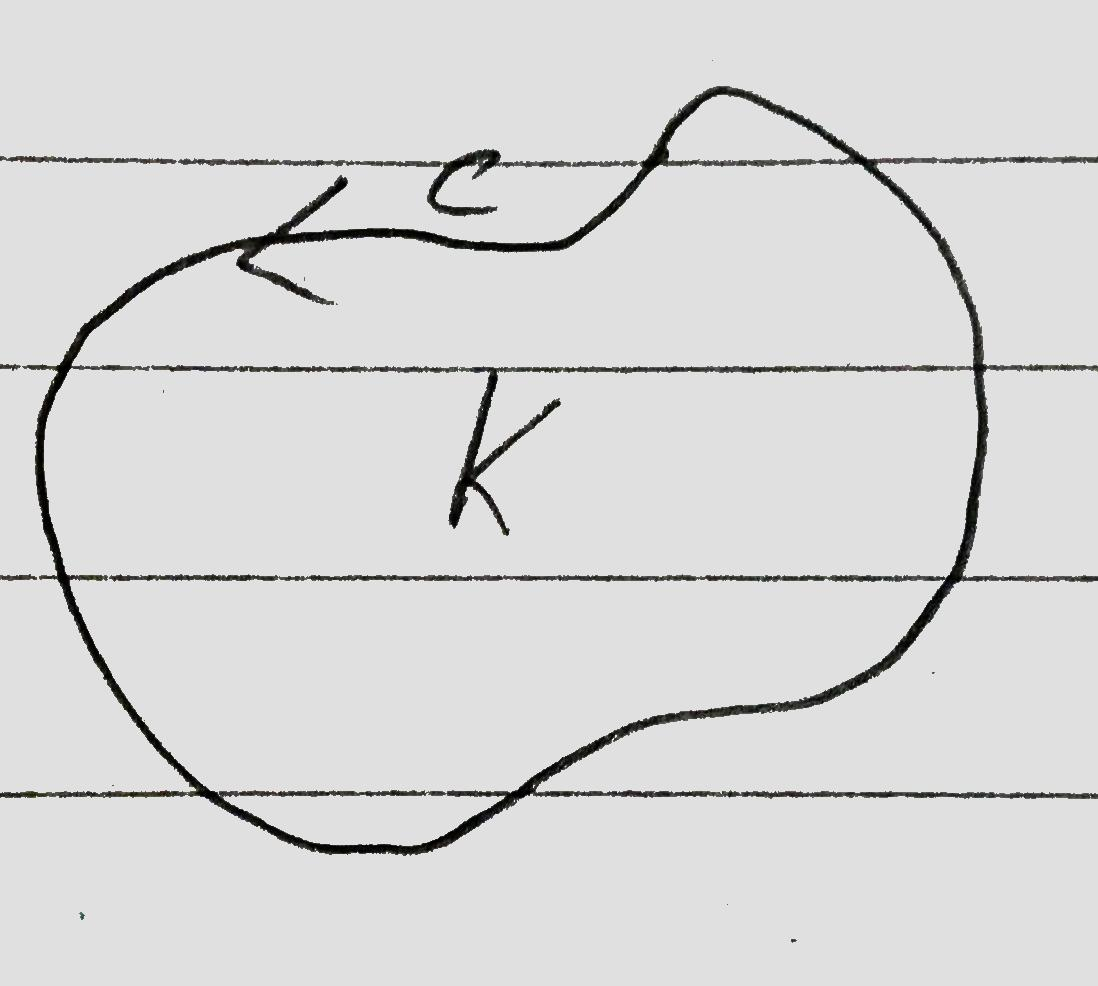
\includegraphics[width=0.25\textwidth]{./img/green_a.jpg}
		  \caption{Durchlaufrichtung}
		  \label{fig:green_a}
	  \end{figure}
	  \begin{bem}
	  	Ist $K\subset \R^2$ ein regulärer Bereich, dann gilt
	  	\begin{equation}
	  		v(K) = \int_{\partial K} x \dy = - \int_{\partial K} y \dx
	  	\end{equation}
	  \end{bem}
	  
	\subsection{Satz von Gauss}
	\subsubsection{Überleitung}
	Der Fluss über den Rand im $\R^2$ ist gegeben durch
	\begin{equation}
		\underbrace{\int_{\partial R} <\vec{F},\vec{n}>\;dr}_{\text{Fluss über den Rand}} = \underset{R}{\int \int}\diverg \vec{F} \;dA
	\end{equation}
	
	Der Fluss über den Rand im $\R^3$ ist gegeben durch
	\begin{equation}
		\underbrace{\underset{\partial R}{\int \int} <\vec{F},\vec{n}>\;dr}_{\text{Fluss über den Rand}} = \underset{R}{\int \int \int}\diverg \vec{F} \;dV
	\end{equation}
	
	\begin{figure}[H] 
		\centering
		\begin{minipage}{.5\textwidth}
		  \centering
		  \captionsetup{justification=centering}
		 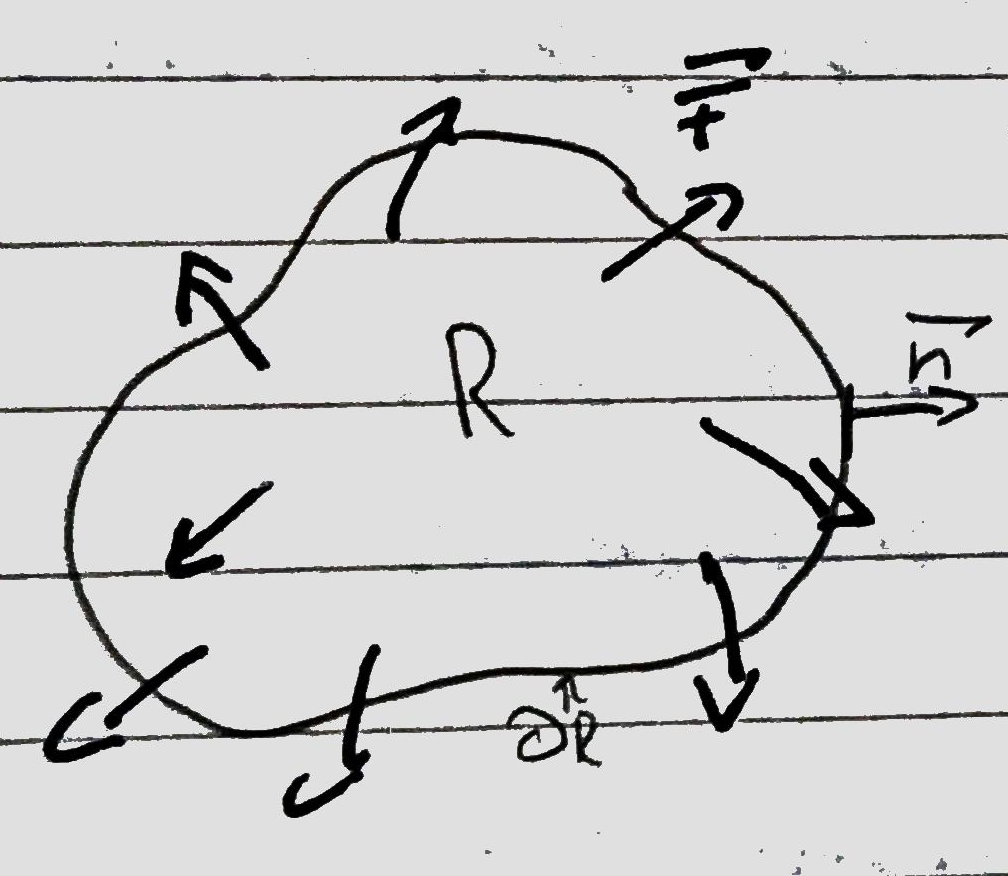
\includegraphics[width=0.6\textwidth]{./img/gauss_a.png}
		  \caption{Fluss über Rand im $\R^2$}
		  \label{fig:gauss_a}
		\end{minipage}%
		\begin{minipage}{.5\textwidth}
		  \centering
		  \captionsetup{justification=centering}
		 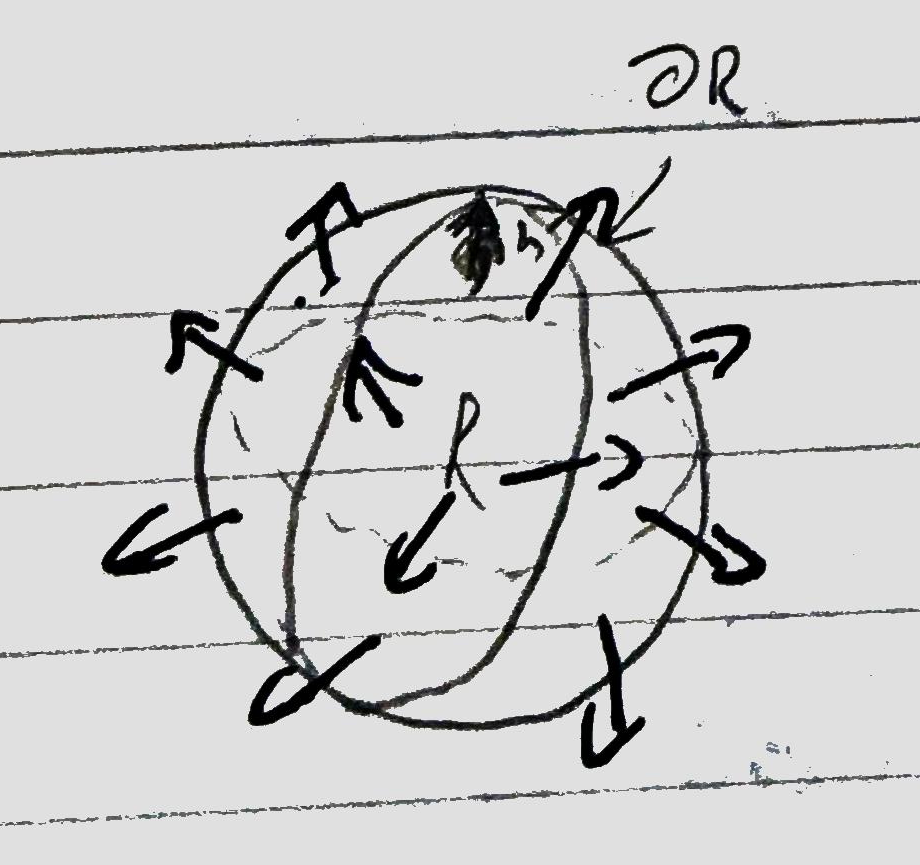
\includegraphics[width=0.55\textwidth]{./img/gauss_b.png}
		  \caption{Fluss über Rand im $\R^3$}
		  \label{fig:gauss_b}
		\end{minipage}
	 \end{figure}
	 
	 \subsubsection{Satz von Gauss (Divergenztheorem)}
	 Ist $B$ ein kompakter Teilbereich des $\R^3$ mit der Oberfläche $\partial B$, die sich auf stückweise stetige Weise parametrisieren lässt, und ist $\vec{v}(\vec{r})$ ein in ganz $B$ stetig differenzierbares Vektorfeld, so gilt, sofern alle vorkommenden Funktionen über die entsprechenden Bereiche integrierbar sind:
	 \begin{equation}
	 	\int_{\partial B} \vec{v} \; \vec{d \sigma} = \int_B \diverg \vec{v} \; d \vec{x}
	 \end{equation}
	 
	 \subsubsection{Satz von Gauss in der Ebene}
	 Für einen kompakten, einfach  zusammenhängenden Bereich $B \subset \R^2$, dessen positiv durchlaufener Rand durch eine stetig diffbare Abbildung $\vec{x} = \vec{x}(t),\;t \in [a,b]$ parametrisiert werden kann, gilt sofern alle beteiligten Funktionen über die entsprechenden Bereiche integrierbar sind
	 \begin{equation}
	 	\int_a^b (v_1(\vec{x}(t)) \frac{dx_2}{dt} - v_2 (\vec{x}(t)) \frac{dx_1}{dt} = \int_B \left( \frac{\partial v_1}{\partial x_1} + \frac{\partial v_2}{\partial x_2}\right) \; d(x_1, x_2)
	 \end{equation}
	 
	 \subsubsection{Satz von Gauss im $R^2$ aus der Vorlesung}
	 Sei $D \subset \R^2$ offen und $\vec{v}:D \to \R^2$ ein $C^1$- Vektofreld. Dann gilt für jeden regulären Bereich $B \subset D$.
	 \begin{equation}
	 	\int_{\partial B} <\vec{v}, \vec{n}>ds =  \int_B \diverg(\vec{v})d(x,y)
	 \end{equation}
	 wobei $|\vec{n}|=1, \vec{n}\perp \partial B$ aus B hinaus zeigt.
	 
	 \subsection{Satz von Stokes}
	 Der Satz von Stokes verknüpft das Kurvenintegral über einen geschlossenen Weg $c$ mit dem Integral der Rotation über eine beliebige von $c$ umrandete Fläche $F$. \newline
	 Für eine orientierbare, stückweise glatte Fläche $F$ mit dem stückweise glatten Rand $\partial F$ und ein auf dem Bild dieser Fläche stetig diffbaren Vektorfeld $\vec{v}$ gilt, sofern alle vorkommenden Funktionen über die entsprechenden Bereiche integrierbar sind
	 \begin{equation}
	 	\oint_{\partial F} \vec{v} \; d\vec{s} = \int_F \rot \vec{v} \; \vec{d \sigma}
	 \end{equation}
	 Dabei ist die Kurve $\partial F$ so parametrisiert, dass sie den nach außen weisenden Normalenvektor $\vec{n} = \frac{\vec{d \sigma}}{d \sigma}$ der Fläche im mathematisch positiven Sinn umläuft.
	 
	 \begin{bem}
	 Einheitsnormalenfeld: Ein Vektorfeld, dass überall auf der Fläche einen Normalenvektor wirken lässt heißt Einheitsnormalenfeld.
	  \begin{figure}[H] 
		  \centering
		  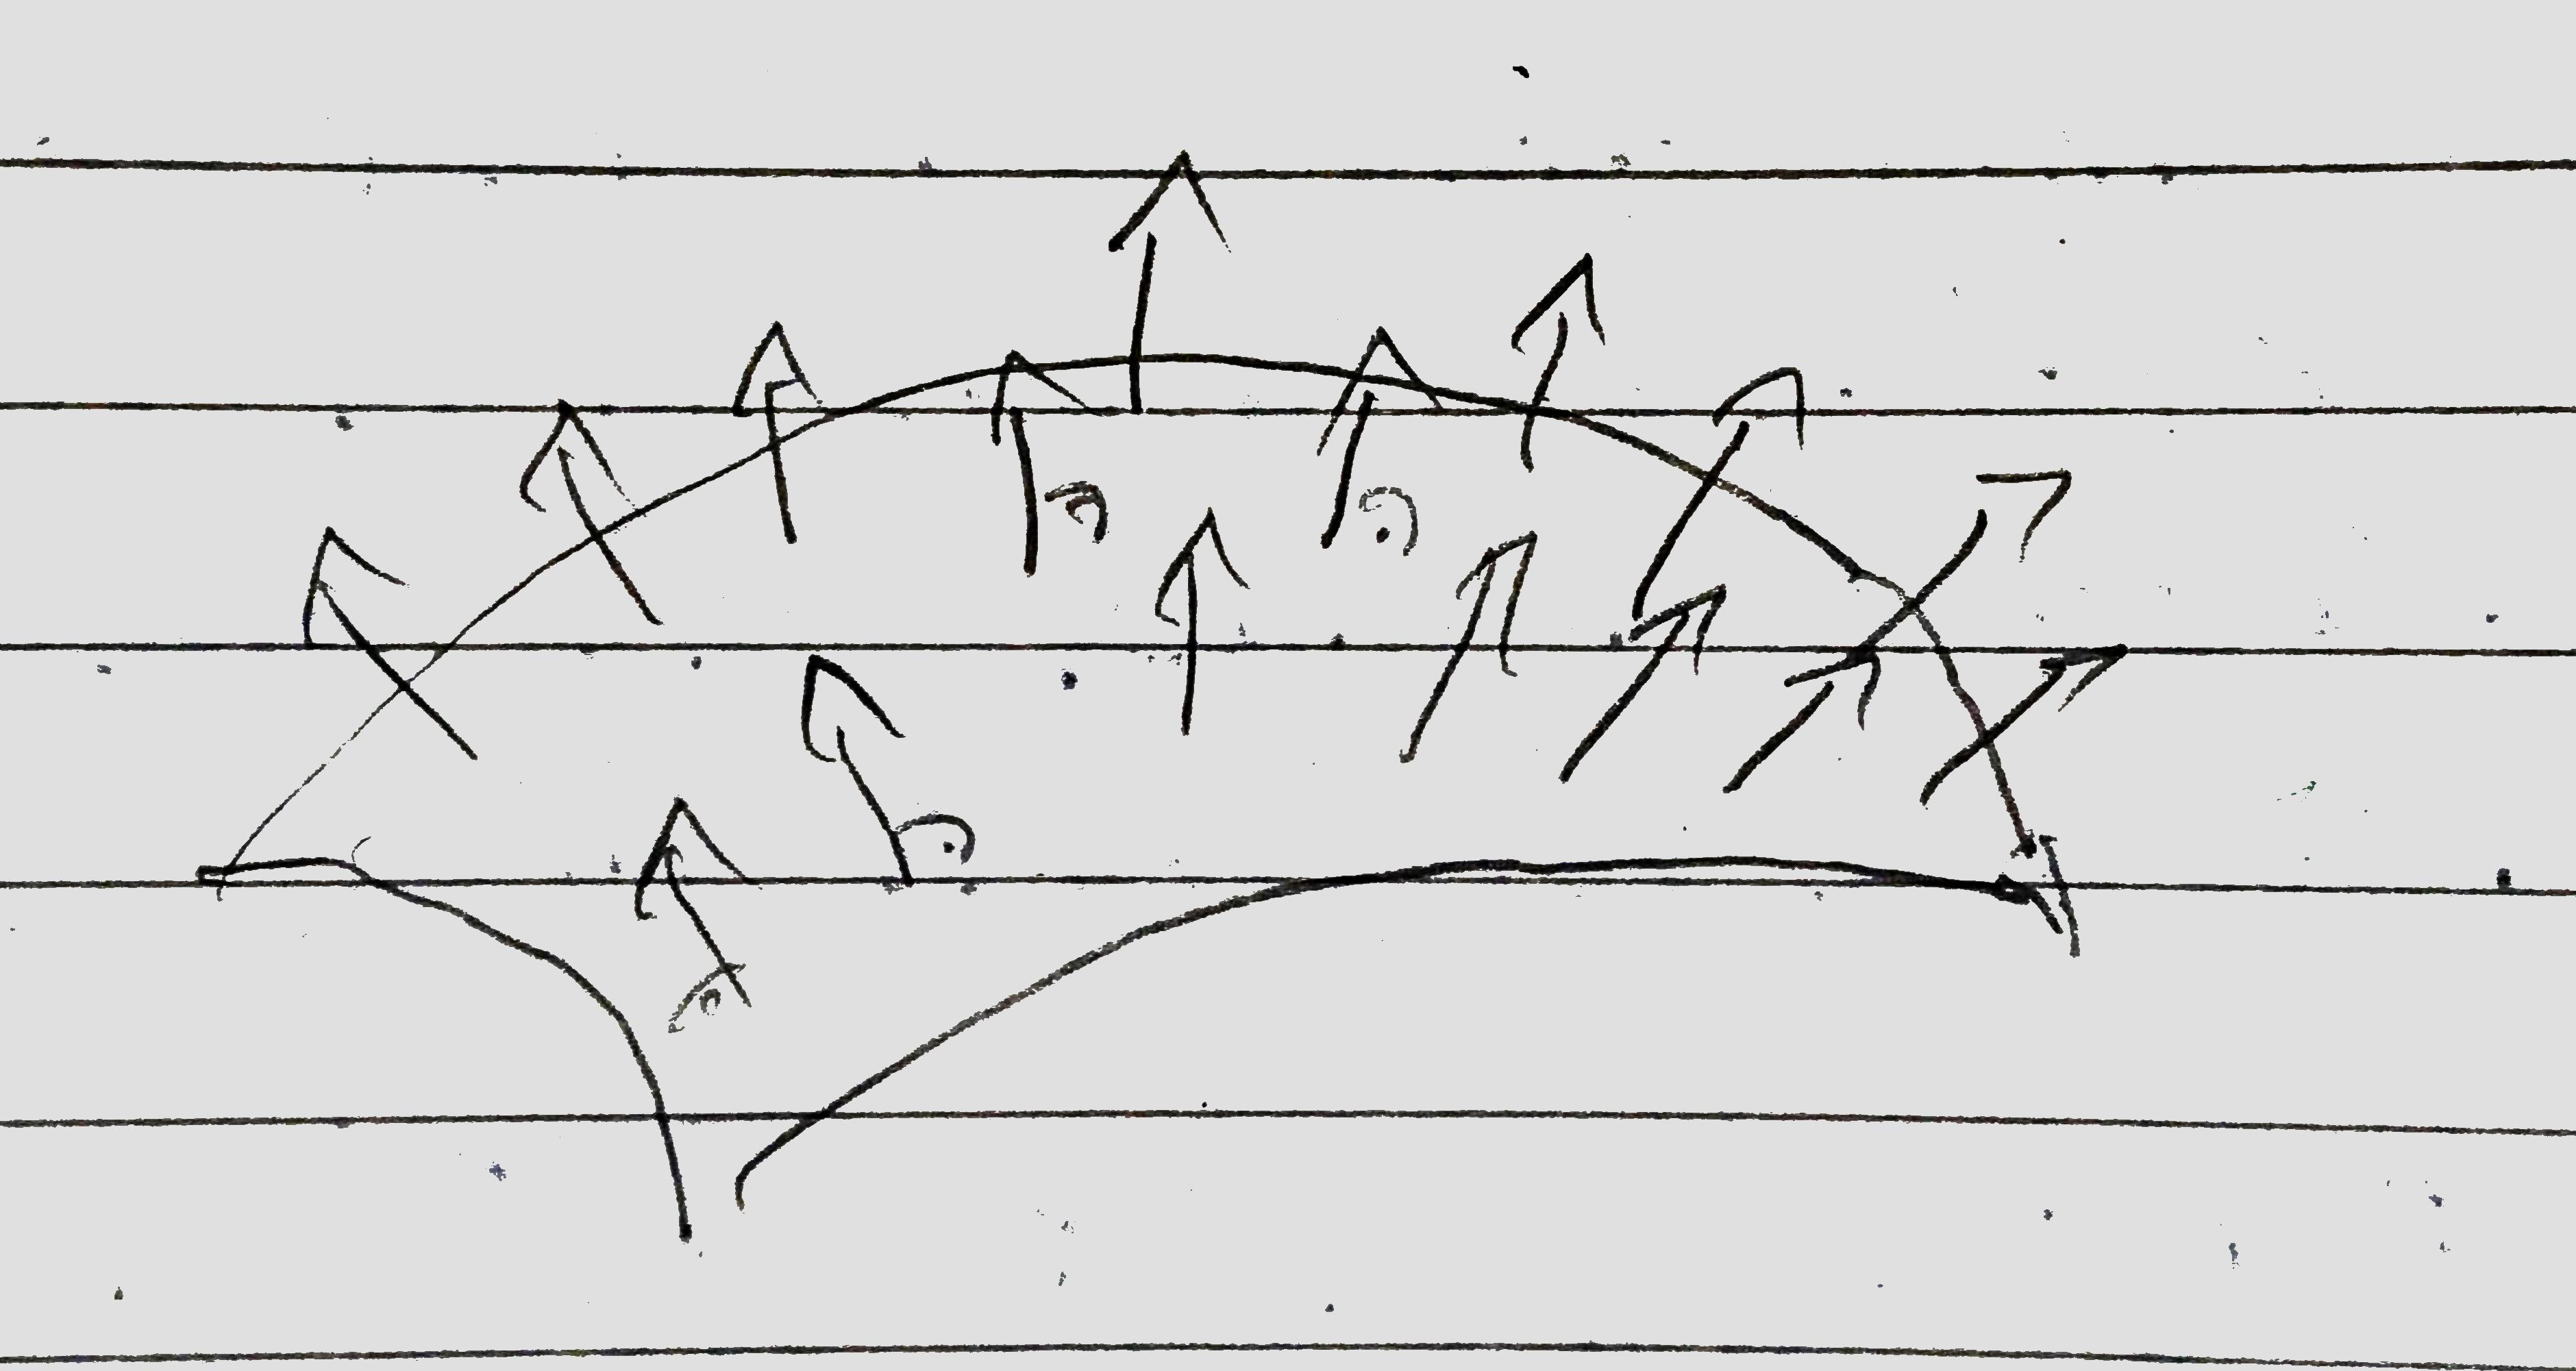
\includegraphics[width=0.5\textwidth]{./img/einheitsnormfeld.png}
		  \caption{Einheitsnormalenfeld}
		  \label{fig:einhNormFeld}
	  \end{figure}
	  \end{bem}
	  %\vspace{-0.5cm}
	  
	  
	  \subsection{Greensche Identität}
	  \begin{equation}
	  	\int_A (f \cdot \lapl g - \lapl f\cdot g)\;d^3 x = \int{\partial A}<f\nabla g - g \nabla f, \vec{n}> d \vec{\sigma}
	  \end{equation}
	  
	  \subsection{Weitere Definitionen}
	  \subsubsection{Regulär}
	  \begin{definition}
	  	Eine Fläche $S \subset \R^3$ heißt stückweise regulär, wenn sie zusammengesetzt ist aus endlich vielen regulären Flächenstücken $s_1 ... s_n$:
	  	\begin{equation}
	  		S = \sum_{i = 1}^n s_i
	  	\end{equation}
	  	wobei sich nur die Ränder berühren dürfen. Der Rand $\partial S$ von $S$ besteht dann per Definition aus allen Randstücken $\partial s_i$ die nur zu einem $s_i$ gehören.
	  \end{definition}
	  
	  
%%first chapter damn im too lazy to think about some good notes to put here
\chapter{HM3} 
	\section{Integralberechnung}
\subsection{Unbestimmtes Integral}
\begin{equation}
\int f(x) dx = F(x) + C = [F(x)]\qquad, C\in\R \label{eq:def_noBorder}
\end{equation}

\subsection{Bestimmtes Integral}
\begin{equation}
\int_a^b f(x) dx = F(b) - F(a) \label{eq:def_border}
\end{equation}

\subsection{Partielle Integration}
Entspricht der "Produktregel" der Differentialrechnung.
\begin{equation}
\int_{\colBord{a}}^{\colBord{b}} f'(x) g(x) dx = f(x) g(x) \colBord{\Big|_a^b} - \int_{\colBord{a}}^{\colBord{b}} f(x) g'(x) dx \label{eq:rule_partInt}
\end{equation}
Bietet sich zum Beispiel bei Produkten aus x-Potenz mit e-Funktionen, log, sin oder cos an.

\subsection{Integration durch Substitution}
Entspricht der "Kettenregel" der Differentialrechnung.
\begin{equation}
\int_{\colBord{a}}^{\colBord{b}} f(g(x))g'(x) dx = \int_{\colBord{g(a)}}^{\colBord{g(b)}} f(y) dy \qquad (setze \quad y = g(x) \label{eq:rule_subs}
\end{equation}

\subsubsection{Spezialfall}
\begin{equation}
\int \frac{f'(x)}{f(x)} dx = ln(|f(x)|) + C \qquad ,C\in\R \label{eq:rule_spec}
\end{equation}

\subsection{Gerade/Ungerade Funktionen}
\begin{align}
\int_{-a}^a f(x) = 
\begin{cases}
2 \int_0^a f(x) dx &,\; f\; gerade\\
0 &,\; f\; ungerade\\
\end{cases} \label{eq:evenodd}
\end{align}
\begin{align*}
\text{f gerade, falls }f(-x) &= f(x) \qquad &(z.B.: cos(x), x^2)\\
\text{f ungerade, falls }f(-x) &= -f(x) \qquad &(z.B.: sin(x), x^3)\\
\end{align*}

\subsection{Allgemeines zur Integration}
\subsubsection{Riemann Integrierbarkeit}
$f:[a,b] \rightarrow \R$ stetig bzw. monoton \newline
$\Rightarrow$ f ist R-integrierbar.

\subsubsubsection{Riemannsches Unterintegral}
\begin{equation}
\int_{a}^{\bar{b}} f(x) dx = \sup\{U_f(Z): \; \text{Z Zerlegung von }[a,b]\}
\end{equation}


\subsubsubsection{Riemannsches Oberintegral}
\begin{equation}
\int_{\bar{a}}^{b} f(x) dx = \inf\{O_f(Z): \; \text{Z Zerlegung von }[a,b]\}
\end{equation}

$\rightarrow \text{f heißt Riemann-integrierbar über }[a,b]$, falls
\begin{equation}
\int_{\bar{a}}^{b} f(x) dx = \int_a^{\bar{b}} f(x) dx
\end{equation}
\newline
In diesem Fall heißt der Wert das Riemannn-Integral und wird mit $\int_a^b f(x)dx$ bezeichnet.

\subsubsubsection{Riemannsche Untersumme}
\begin{equation}
  U_f(Z) = \sum_{j = 0}^{n-1} \inf\limits_{\xi \in [x_j, X_{j+1}]} f(\xi) \cdot (x_{j+1} -x_j)
\end{equation}
\subsubsubsection{Riemannsche Obersumme}
\begin{equation}
  O_f(Z) = \sum_{j = 0}^{n-1} \sup\limits_{\xi \in [x_j, X_{j+1}]} f(\xi) \cdot (x_{j+1} -x_j)
\end{equation}

\subsubsubsection{Eigenschaften}
\begin{description}
\item[a)]
Falls $a<b$ setzen wir:
\begin{align}
\int_b^a f(x) dx &= -\int_a^bf(x)dx \nonumber \\
\int_a^a f(x) dx &= 0
\end{align}
\item[b)]
f, g seien R-integrierbar, $\lambda , \mu \in \R \rightarrow \lambda f + \mu g$ ist R-integrierbar (Vektorraumeigenschaft).
\begin{equation}
\int_a^b \lambda f + \mu g)(x)dx = \lambda \int_a^b f(x) dx + \mu \int_a^b g(x) dx
\end{equation}
\item[c)]
$a<C<b$, f ist R-integrierbar.
\begin{equation}
\int_a^b f(x) dx = \int_a^C f(x) dx + \int_C^b f(x) dx
\end{equation}
\item[d)]
\begin{align}
f(x) \ge 0 &\Rightarrow \int_a^b f(x) dx \ge 0 \nonumber \\
f(x) \ge g(x) &\Rightarrow \int_a^b f(x) dx \ge \int_a^b g(x)dx
\end{align}
\item[e)]
\begin{equation}
\text{Sind $f$ und $g$ R-integrierbar ist auch $f*g$ R-integrierbar.}
\end{equation}
\item[f)]
\begin{align}
g(x) \ge C > 0 \Rightarrow \frac{f}{g} \text{ ist R-integrierbar.}
\end{align}
\item[g)]
\begin{equation}
\text{Ist $f$ R-integrierbar dann ist auch } |f| \text{ R-integrierbar.}
\end{equation} 
\item[h)]
\begin{equation}
(b-a) \inf_{x\in[a,b]}{f(x)} \le \int_a^b f(x) dx \le (b-a) \sup_{x\in [a,b]}{f(x)}
\end{equation}
\end{description}

\subsubsubsection{Kriterien zur Riemann-Integrierbarkeit}

\begin{description}
\item[a)]
$f$ monoton $\Rightarrow f$ R-integrierbar.
\item[b)]
$f$ stetig $\Rightarrow f$ R-integrierbar
\begin{satz}
\glqq Jede stetige Funktion $f:k \rightarrow \R$ auf einer kompakten Menge k, d.h. für $k<\R^d$ abgeschlossen und beschränkt, ist dort gleichmäßig stetig und damit R-integrierbar.\grqq \cite{HM12}
Beispiel für k: $k:[a,b]$
\end{satz}
\item[c)]
\begin{satz}
Kriterium: Jede Funktion deren Unstetigkeitsstellen eine Nullmenge bilden (z.B. abzählbare Mengen) sind R-integrierbar.
\glqq Satz: Eine Funktion $f:[a,b]\rightarrow \R$ ist genau dann R-integrierbar, wenn $f$ beschränkt ist und die Menge der Unstetigkeitsstellen eine Nullmenge ist. 
\grqq \cite{HM12}
\end{satz}
Die Konsequenz daraus lautet, dass jede stetige Funktion mit endlich vielen Sprungstellen R-integrierbar ist. \citeVgl{HM12}
\item[d)]
\begin{satz}
\glqq Sei $f:[a,b] \rightarrow \R$ beschränkt. Dann ist $f$ R-integrierbar genau dann, wenn es zu jedem $\varepsilon > 0$ eine Partition $Z$ gibt, 
so dass
$O_f(Z)  U_f(Z) < \varepsilon$. \grqq \cite{HM12}
\end{satz}
Anmerkung: \glqq In der Mengenlehre ist eine Partition (auch Zerlegung oder Klasseneinteilung) einer Menge M eine Menge P, deren Elemente nichtleere Teilmengen von M sind, sodass jedes Element von M in genau einem Element von P enthalten ist. Anders gesagt: Eine Partition einer Menge ist eine Zerlegung dieser Menge in nichtleere paarweise disjunkte Teilmengen.\grqq  \cite{wiki}

\end{description}

\subsubsection{MWS der Integralrechnung}
$f:[a,b]\rightarrow\R$ stetig, dann $\exists \; \xi \in[a,b]$ mit $\int_a^b f(x)dx = f(\xi)(b-a)$.

\subsubsection{Hauptsatz der Differential- und Integralrechnung}
$f:[a,b]\rightarrow\R$ stetig, dann ist $F(x) = \int_a^x f(t)dt$ diffbar und $F'(x) = f(x)$.

\subsubsubsection{Folgerungen}
\begin{satz}
Ist $f$ ungerade, so ist $f''$ gerade, und alle Stammfunktionen vonm $f$ sind gerade.\citevgl{HM2Vortragsubung}
\end{satz}
\begin{satz}
Ist $f$ gerade, so ist $f'$ ungerade, und $f$ besitzt eine ungerade Stammfunktion.\citevgl{HM2Vortragsubung}
\end{satz}

\subsection{Partialbruchzerlegung}
	\begin{equation}
	  R(x) = \frac{p(x)}{q(x)}, \qquad p,q\text{ Polynome}
	\end{equation}
	Vorgehensweise:
	\begin{description}
	  \item{\textbf{1)}} Zähler und Nennergrad untersuchen\newline
	  ist $grad(p) > grad(q)$, also Zählergrad > Nennergrad umformen in  \newline$R(x) = p_1(x) + \frac{p_2(x)}{q(x)}$ $\Rightarrow$ Polynomdivision.
	  \item{\textbf{2)}} Nullstellen und faktorisieren
	    \begin{itemize}
	      \item Nullstellen des Nenners bestimmen
	      \item Nenner Faktorisieren in $p1, p2, ...$
	    \end{itemize}
	  \item{\textbf{3)}} Ansatz
	    \begin{itemize}
	      \item Ansatz für Partialbruchzerlegung $R(x) = \frac{A}{p1} + \frac{B}{p2} + ...$
	      \item Bestimmung von A, B, C, ...
	    \end{itemize}
	\end{description}
  Bei quadratischen oder höhergradigen Nullstellen lautet der Ansatz:
  \begin{equation}
    NST = x^n \Rightarrow R(x) = \frac{A}{x} + \frac{B}{x^2} + ... + \frac{N}{x^n}
  \end{equation}
  Bei komplexen Nullstellen muss der Ansatz angepasst werden.
  \begin{align}
    &NST: 2, -2, 2i, -2i \nonumber \\
    &Ansatz: R(x) = \frac{A}{x-2} + \frac{B}{x+2} + \frac{Cx + D}{x^2+4}
  \end{align}
  Es werden also die komplexen Nullstellen ausmultipliziert und so reell dargestellt.
  
\subsection{Uneigentliche Integrale}
  \begin{satz}
    Sei $f:[a, \infty] := I \rightarrow \R$ lokal integrierbar. Konvergiert $\int_a^\infty f(x) dx$ absolut. d.h. ist $\int_a^\infty |f(x)| dx$ konvergent, so konvergiert auch $\int_a^\infty f(x) dx$.
  \end{satz}
  \begin{satz}
    Majorantenkriterium: Gilt für alle $x\in I$, dass $|f(x)| \leq g(x)$, und ist $\int_a^\infty g(x) dx$ konvergent, so ist $\int_a^\infty dx$ (im Script vom Prof ist hier die untere Grenze 0, ich denke es sollte aber a sein) absolut konvergent.    
  \end{satz}
  \begin{satz}
    Minorantenkriterium: Gilt für alle $x\in I$, dass $0 \leq g(x) \leq f(x)$ und divergiert $\int_a^\infty g(x) dx$, so divergiert auch $\int_a^\infty dx$.
  \end{satz}
  \begin{bem}
    Abschätzungen mit negativen Minoranten sind falsch da mit einer negativen Minorante alles nach unten abgeschätzt werden kann.
  \end{bem}
  \subsubsection{Typen uneigentlicher Integrale}
  \begin{align}
    \textbf{\colGreen{Singularität:} }\int_{\colGreen{0}}^1 \frac{1}{\sqrt{\colGreen{x}}} dx \nonumber \\
    \textbf{\colGreen{Unbeschränktes Gebiet:} }\int_1^{\colGreen{\infty}} e^{-x} dx \nonumber \\
  \end{align}
  \begin{definition}
    Eine Singularität ist die Stelle, an der die Funktion divergieren würde oder undefiniert wäre.
  \end{definition}
  \textbf{Methode:} Ersetzen der kritischen Stelle durch $z$ und setzen eines Grenzüberganges, z.B.:
  \begin{align*}
    \lim\limits_{z\rightarrow0} \int_z^1 \frac{1}{\sqrt{x}} dx, \quad \lim\limits_{z\rightarrow \infty} \int_1^z e^{-x} dx
  \end{align*}
  \textbf{Vergleichsintegrale}
  \begin{align}
    \int_1^\infty \frac{1}{x^\alpha} dx = 
    \begin{cases}
      \text{konvergiert}\quad , \alpha > 1 \\
      \text{divergiert}\quad , \alpha \leq 1
    \end{cases} \nonumber\\
    \int_0^1 \frac{1}{x^\alpha} dx = 
    \begin{cases}
      \text{divergiert}\quad , \alpha \geq 1 \\
      \text{konvergiert}\quad , \alpha < 1
    \end{cases} \nonumber\\    
  \end{align}

\subsection{Wichtige Integrale}
\begin{equation}
  \int \frac{1}{1+y^2} dx = arctan(y)
\end{equation}
\begin{equation}
  \int x^n dx = \frac{x^{n+1}}{n+1}, \qquad n \neq -1
\end{equation}
\begin{equation}
  \int \frac{1}{cos^2(x)} dx = tan(x)
\end{equation}
\begin{equation}
  \int \frac{1}{sin^2(x)} dx = cot(x)
\end{equation}
\begin{equation}
  \int a^x dx = \frac{a^x}{ln(a)}
\end{equation}
\begin{equation}
  \int \frac{1}{x} dx = ln|x|
\end{equation}
\begin{equation}
  \int \frac{1}{cosh^2(x)} dx = tanh(x)
\end{equation}
\begin{equation}
  \int \frac{1}{sinh^2(x)} dx = -coth(x)
\end{equation}
\begin{equation}
  \int ln(x) dx = x ln(x) -x
\end{equation}
\begin{equation}
  \int \frac{1}{x-x_1} dx = ln|x-x_1|
\end{equation}
\begin{equation}
  \int \frac{1}{/x-x_1)^k} dx = \frac{1}{-k+1}(x-x_1)^{-k+1}, \quad k>1
\end{equation}
\begin{equation}
  \int \frac{1}{(x-a)^2+b^2}dx = \frac{1}{b^2} \int \frac{1}{\left(\frac{x-a}{b}\right)^2 +1} dx = \frac{1}{b} arctan\left(\frac{x-a}{b}\right)
\end{equation}

\subsection{Separierbare DGL}
  \subsubsection{Wiederholung klassische DGL}
  Bisher: lineare DGl mit konstanten Koeffizienten. \newline
  z.B.: $y''(t) - 5y'(t) + 4y(t) = e^{\colGreen{2}t} \qquad ,\; y(0) = 1,\; y'(0) = 1$ \newline
  \begin{tabularx}{14.7cm}{l l}
	  Homogene DGL: & $y(t) = e^{\lambda t} \Rightarrow p(\lambda) = \lambda^2 - 5 \lambda +4 = 0$ \\
	  $\;$ & $\Rightarrow \lambda_1 = 1, \; \lambda_2 = 4$ \\
	  $\;$ & $\Rightarrow yh(t) = C_1 e^t + C_2 e^{4t} \qquad ,\;C_1,\;C_2 \in \R$\\
	  $\;$ & $\;$ \\
	  Inhomogenes DGL: & $\ubGreen{\text{da 2 keine NST}}{yp(t) = re^{2t}}$\\
  \end{tabularx}  
  \begin{align*}
    &\Rightarrow yp'(t) = 2re^{2t},\; yp''(t) = 4re^{2t} \\
    &\overset{DGL}{=} 4re^{2t} - 10re^{2t} + 4re^{2t} \overset{!}{=} e^{2t} \Rightarrow -2re^{2t} = e^{2t}\\
    &\Rightarrow r = -\frac{1}{2}
  \end{align*} 
  \begin{tabularx}{14.7cm}{l l}
	  Allgemeine Lösung: & $y(t) = yh(t) + yp(t) = C_1 e^t + C_2 e^{4t} - \frac{1}{2} e^{2t}$
  \end{tabularx}
  
  \subsubsection{Lösen von DGL mit Koeffizienten die von t abhängig sind}
  z.B. $ y'(t) - ty(t) = t \qquad ,\; y(0) = 1$\newline
  \newline
  Spezielle Form: 
  \begin{equation}
    y'(t) = f(t) g(y(t)) \qquad,\; y(t_0) = y_0
  \end{equation}     
  \begin{align*}
    \Rightarrow y'(t) = t+ty(t) = \ubGreen{f(t)}{t} \ubGreen{(1+y(t))}{g(y(t))}
  \end{align*}
  Lösung: Trennung der Veränderlichen:
  \begin{align}
  \frac{y'}{g(y)} = f(t) \overset{\colGreen{y' = \frac{dy}{dt}}}{\Rightarrow} \colGreen{\int} \frac{1}{g(y)} dy = \colGreen{\int} f(t)dt +C \quad ,\;C\in\R
  \end{align}
  $C$ erhält man aus der Anfangsbedingung $y(t_0) = y_0$.
  \newpage
	
	\section{Laplace Operator}
	\subsection{Laplace in karthesischen Koordinaten}
	\begin{equation}
		\lapl \varphi = \nabla \nabla \varphi= \sum\limits_{j=1}^d \frac{\diffp^2 \varphi}{\diffp x_j^2} = \frac{\diffp^2 \varphi}{\diffp x_1^2} + ... + \frac{\diffp^2 \varphi}{\diffp x_d^2}
	\end{equation}
	
	\subsection{Laplace in Polarkoordinaten}
	\begin{equation}
		\lapl = \frac{1}{r} \frac{\partial}{\partial r} r \frac{\partial }{\partial r} + \frac{1}{r^2}\frac{\partial^2}{\partial \varphi^2 }
	\end{equation}

	\subsection{Laplace in Zylinderkoordinaten}
	\begin{equation}
		\lapl =\frac{1}{\rho} \frac{\partial}{\partial \rho}
\left( \rho\,\frac{\partial f}{\partial \rho} \right) +
\frac{1}{\rho^2}\frac{\partial^2 f}{\partial \varphi^2} +
\frac{\partial^2 f}{\partial z^2}
	\end{equation}
	
	\subsection{Laplace in Kugelkoordinaten}
	\begin{equation}
		\lapl = \frac{1}{r^2} \frac{\partial}{\partial r}r^2 \frac{\partial}{\partial r} + \frac{1}{r^2 sin \vartheta}\frac{\partial}{\partial \vartheta} sin \vartheta \frac{\partial}{\partial \vartheta} + \frac{1}{r^2 \sin^2 \vartheta}\frac{\partial^2}{\partial \varphi^2}
	\end{equation}
	
	\subsection{Laplace in Elliptischen Koordinaten}
	\begin{equation}
		\lapl = \frac{1}{a^2(\sinh^2 (u) \cos^2(v)+\cosh^2 (u) \sin^2(v))} \left( \frac{\partial^2}{\partial^2 u} + \frac{\partial^2}{\partial^2 v}\right)
	\end{equation}
		
	\subsection{Laplace Beltrami Operator}
	Ist $f \in C^2(V))$ dann gilt $\tilde{\lapl f} = \tilde{\lapl} \tilde{f}$ wobei
	\begin{align}
		\tilde{\lapl} &=  \frac{1}{\sqrt{g(u)}} \sum_{k,l}^n \frac{\partial}{\partial u_k} \sqrt{g(u)} \;\; g^{kl} \frac{\partial}{\partial u_l} \nonumber \\
		&= \frac{1}{\sqrt{g(u)}}\sum_{k=1}^n \sum_{l=1}^n \left( \frac{\partial}{\partial u_k} \sqrt{g(u)} \;\; g^{kl} \frac{\partial}{\partial u_l} \right) \label{eq:lapl_beltr}
	\end{align}
	Wobei $g(u) = \det G(u)$ ist. $g_{kl}$ sind dabei die einzelnen Komponenten von $G(u)$. $g^{kl}$ sind die Komponenten der Inversen von $G(u)$. \newline
	Weiterhin gilt 
	\begin{equation}
		G(u) = J_{\vec{x}}^T \cdot J_{\vec{x}}
	\end{equation}
	Man nennt $G(u)$ die Grahmsche Matrix. $\vec{x}$ ist hierbei die Transformationsabbildung. 
	
	\subsubsection{Ablauf am Beispiel der Polarkoordinaten}
	Parametrisierung: $\vec{x} = \vecT{r \cos \varphi \\ r \sin \varphi}$
	\begin{flalign*}
    &\textbf{Schritt 1: } \text{Jacobi -Matrix bilden und transponieren:}&
  \end{flalign*}
    \vspace{-0.5cm}
  \begin{flalign*}
  	& J_{\vec{x}} = \left( 
	  \begin{array}{c c}
  	  	\cos\varphi & -r\sin \varphi \\
  	  	\sin \varphi & r \cos \varphi	
  	 \end{array} \right) \quad \Rightarrow \quad J_{\vec{x}}^T = \left( 
  	 \begin{array}{c c}
  	 	\cos \varphi & \sin \varphi \\
  	 	-r \sin \varphi & r \cos \varphi
  	 \end{array} \right)
  \end{flalign*}
    \vspace{-0.5cm}
  \begin{flalign*}
    &\textbf{Schritt 2: } \text{Grahmsche Matrix bestimmen}&
  \end{flalign*}
    \vspace{-0.5cm}
  \begin{align*}
    G = J_{\vec{x}}^T J{\vec{x}} = \left( 
    \begin{array}{c c}
    		1 & 0\\
    		0 & r^2
    \end{array} \right)
  \end{align*}
    \vspace{-0.5cm}
  \begin{flalign*}
    &\textbf{Schritt 3: } \text{Inverse bestimmen}&
  \end{flalign*}
    \vspace{-0.5cm}
  \begin{align*}
     G ^{-1} = \frac{1}{r^2} \left( 
     \begin{array}{c c}
     	r^2 & 0 \\
     	0 & 1
     \end{array} \right) \quad = \quad \left(
     \begin{array}{c c}
     	1 & 0\\
     	0 & \frac{1}{r^2}
     \end{array}\right)
  \end{align*}
    \vspace{-0.5cm}
  \begin{flalign*}
    &\textbf{Schritt 4: } \text{In Laplace-Beltrami Operator einsetzen}&
  \end{flalign*}
    \vspace{-0.5cm}
  \begin{align*}
     \tilde{\lapl} &= \frac{1}{r} \left( \underbrace{\left( \frac{\partial}{\partial r}r \cdot \overbrace{1}^{g^{11}} \frac{\partial}{\partial r}\right)}_{k=1,\;l=1} +
    \underbrace{\left(\frac{\partial}{\partial r} r \cdot \overbrace{0}^{g^{12}} \cdot \frac{\partial}{\partial \varphi}\right)}_{k=1,\;l=2} +
    \underbrace{\left(\frac{\partial}{\partial \varphi} r \cdot \overbrace{0}^{g^{21}} \cdot \frac{\partial}{\partial r}\right)}_{k=2,\;l=1} +
    \underbrace{\left(\frac{\partial}{\partial \varphi} r \cdot \overbrace{\frac{1}{r^2}}^{g^{22}} \cdot \frac{\partial}{\partial \varphi}\right)}_{k=2,\;l=2} \right) \\
    &= \frac{1}{r} \frac{\partial}{\partial r}r \frac{\partial}{\partial r} + \frac{1}{r}\frac{\partial}{\partial \varphi} \frac{\cancel{r}}{r^{\cancel{2}}} \frac{\partial}{\partial \varphi} =\frac{1}{r} \frac{\partial}{\partial r} r \frac{\partial }{\partial r} + \frac{1}{r^2}\frac{\partial^2}{\partial \varphi^2 } 
  \end{align*}
	\section{Mehrdimensionale Analysis}
  \subsection{Partielle Ableitung}
  \begin{definition}
    $f(x)$ heißt in $x^* \in \R^d$ nach der $j-ten$ Koordinate $x_j$ partiell diffbar, falls der Grenzwert
    \begin{equation}
      \frac{\partial f}{\partial x_j}(x^*) = \lim\limits_{t\rightarrow 0} \frac{f(x^* + t e_j) - f(x^*)}{t}
    \end{equation}
    existiert bzw. falls $\tilde{f}_j(x_j)$ in $x_j$ diffbar ist. $\frac{\partial f}{\partial x_j}(x^*)$ heißt die partielle Ableitung von $f$. 
  \end{definition}
  \begin{bem}
    Alternative Schreibweisen:
    \begin{equation}
      \frac{\partial f}{\partial x_j} = \frac{partial}{\partial x_j} f = \partial_{x_j} f = D_j f  = f_{x_j} = ...
    \end{equation}
  \end{bem}
  \begin{definition}
    Allgemein: n-te partielle Anleitung:
    \begin{equation}
      \frac{\diffp^2f}{\diffp x_k \diffp x_j} = \frac{\diffp f}{\diffp x_k}\left(\frac{\diffp f}{\diffp x_k} \right)
    \end{equation}
  \end{definition}
  
  \subsubsection{Gradient und Nabla Operator}
  \begin{definition}
    Der Zeilenvektor
    \begin{equation}
      \grad f(x^*) = \left( \dfp{f}{x_1}(x^*), ..., \dfp{f}{x_d}(x^*)\right)
    \end{equation}
    heißt der Gradient von $f$ in $x^*$. Es gilt weiter:
    \begin{equation}
      \nabla f(x^*) = (\grad f(x^*))^T
    \end{equation}
    Der eingeführte Operator heißt Nabla-Operator.
  \end{definition}
  \begin{satz}
    Sei $f:\R^d \rightarrow \R$ diffbar, dann gilt:
    \begin{itemize}
      \item[a) ] Der Gradientenvektor $\nabla f(x^*)$ steht senkrecht auf der Niveaumenge $N_{x^*} = \lbrace x \in \R^d: f(x) = f(x^*)\rbrace$
      \item[b) ] $\nabla f(x^*)$ gibt die Richtung des steilsten Anstiegs von $f(x)$ im Punkt $x^*$ an.
    \end{itemize}
  \end{satz}
  \begin{bem}
    Es gilt weiterhin:
    \begin{align}
      \grad(\alpha f + \beta g) &= \alpha \grad f + \beta \grad f, \qquad \alpha, \beta \in \R    \\  
      \grad (f\cdot g) &= f \cdot \grad g + g \cdot \grad f
    \end{align}
  \end{bem}
  
  \subsubsection{Jacobi Matrix}
  \begin{definition}
    Die Matrix der ersten Ableitung heißt die Jacobi Matrix. 
    \begin{equation}
      Jf = \left(\begin{array}{c c c}
      \dfp{f_1}{x_1} & \dots  & \dfp{f_1}{x_d} \\
      \vdots         & \ddots & \vdots         \\
      \dfp{f_m}{x_1} & \dots  & \dfp{f_m}{x_d} \end{array}\right)
    \end{equation}
  \end{definition}
  
  \subsection{Richtungsableitung}
  \begin{definition}
    Sei $f: \R^d \rightarrow \R$. Für $x^* \in \R^d$ und $v \in \R^d _{/ \lbrace 0 \rbrace}$ heißt
    \begin{equation}
      D_v f(x^*) = \lim\limits_{t\rightarrow 0} \frac{f(x^* +tv)-f(x^*)}{t}
    \end{equation}
    die Richtungsableitung von $f$ in $x^*$ in Richtung $v$. (Andere Schreibweise: $\dfp{f}{v})$
  \end{definition}
  Wenn alle Ableitungen existieren gilt:
  \begin{equation}
    D_v f = \grad f \cdot v
  \end{equation}
  \begin{bem}
    Der Gradient zeigt dabei selbst in Richtung des steilsten Anstiegs.
  \end{bem}
  
  \begin{satz}
    Ist $f: D\rightarrow \R$ mit $D \subset \R^d$ offen in einer Umgebung von $x^* \in D$ partiell diffbar und sind die partiellen Ableitungen dort beschränkt, dann ist $f$ stetig in $x^*$.
  \end{satz}
  
  \begin{satz}
    Existieren in einer Umgebung von $x^*$ alle partiellen Ableitungen und sind dann stetig in $x^*$, so ist $f$ diffbar in $x^*$. Allgemein gilt, existieren alle partiellen Ableitungen bis zur Ordnung $k$ und sind diese stetig, so ist $f \in C^k$, d.h. $k-fach$ stetig diffbar.
  \end{satz}
  
  \begin{bem}
    Folgerung: Alle Polynome, alle sin, cos, exp, ... Funktionen sind mehrdimensional diffbar.
  \end{bem}
  
  \begin{bem}
    Ist $f:\R^2 \rightarrow \R$ in einer Umgebung $U$ von $x^*$ partiell diffbar und sind diese in $x^*$ stetig, so ist $f$ diffbar in $x^*$.
  \end{bem}
  
  \subsection{Mehrdimensionale Kettenregel}
  \begin{satz}
  Sei $f: \R^n \rightarrow \R^m$ und $g: \R^m \rightarrow \R^d$. Sei $f$ in $x^*$ diffbar und $g$ in $y^* = f(x^*)$ diffbar. Dann ist $g \circ f$ in $x^*$ diffbar mit Jacobimatrix.
  \begin{equation}
    J(g \circ f) (x^*) = Jg(f(x^*)) \cdot Jf(x^*)\label{eq:mehrd_kettenr_jac}
  \end{equation}
  Somit gilt für $h(x) = g(f(x))$, dass
  \begin{equation}
    \dfp{z_{\colRed{k}}}{x_{\colBord{j}}} = \sum\limits_{\colBlue{i}} \dfp{z_{\colRed{k}}}{y_{\colBlue{i}}} \cdot \dfp{y_{\colBlue{i}}}{x_{\colBord{j}}}
  \end{equation}
  \end{satz}
  Vorgehen mit Jacobimatrix:\newline
  Es sei gegeben:
  \begin{align*}
    g: \R^2 \rightarrow \R ,\quad g(x,y) = f(x^2y, x+2y)
  \end{align*}
  \begin{flalign*}
    &\textbf{Schritt 1: } \text{Zur Übersichtlichkeit gegebenenfallsneue Funktionen definieren}&
  \end{flalign*}
  \vspace{-0.5cm}
  \begin{align*}
    q(x,y):= (x^2y, x+2y) \Rightarrow g(x,y) = f(q(x,y))
  \end{align*}
  \vspace{-0.5cm}
  \begin{flalign*}
    &\textbf{Schritt 2: } \text{Jacobimatrix der inneren Funktion aufstellen}&
  \end{flalign*}
  \vspace{-0.5cm}
  \begin{align*}
    Jq(x,y) = \left( \begin{array}{c c}
    2yx & x^2 \\
    1 & 2
    \end{array} \right)
  \end{align*}
  \vspace{-0.5cm}
  \begin{flalign*}
    &\textbf{Schritt 3: } \text{Jacobimatrix der äußeren Funktion in Abhängigkeit von der Inneren aufstellen}&
  \end{flalign*}
  \vspace{-0.5cm}
  \begin{align*}
    J_f(q(x,y)) = \left(\begin{array}{c c}
      \frac{\diffp f}{\diffp x}(q(x,y)) & \frac{\diffp f}{\diffp y} (q(x,y))
    \end{array}\right)
  \end{align*}
   \vspace{-0.5cm}
  \begin{flalign*}
    &\textbf{Schritt 4: } \text{\eqref{eq:mehrd_kettenr_jac} anwenden}&
  \end{flalign*}
  \vspace{-0.5cm}
  \begin{align*}
    J_g(x,y) = J_f(q(x,y)) \cdot J_q(x,y) = \left(\begin{array}{c c}
      \frac{\diffp f}{\diffp x}(q(x,y)) & \frac{\diffp f}{\diffp y} (q(x,y))
    \end{array}\right) \cdot
    \left( \begin{array}{c c}
    2yx & x^2 \\
    1 & 2
    \end{array} \right)
  \end{align*}  \vspace{-0.5cm}
  \begin{flalign*}
    &\textbf{Schritt 5: } \text{Ausmultiplizieren}&
  \end{flalign*}
  \vspace{-0.5cm}
  \begin{align*}
    J_g(x,y) &= 
    \left(
    \begin{array}{c c}
      2yx \frac{\diffp f}{\diffp x}(q(x,y)) + \frac{\diffp f}{\diffp y} (q(x,y)) & x^2 \frac{\diffp f}{\diffp x}(q(x,y)) + 2 \frac{\diffp f}{\diffp y (q(x,y))}
    \end{array}
    \right)\\
    \Rightarrow \frac{\diffp g}{\diffp x} (x,y) &= 2yx \frac{\diffp f}{\diffp x}(q(x,y)) + \frac{\diffp f}{\diffp y} (q(x,y)) \qquad \frac{\diffp g}{\diffp y} = x^2 \frac{\diffp f}{\diffp x}(q(x,y)) + 2 \frac{\diffp f}{\diffp y (q(x,y))}
  \end{align*}  
  
  \subsection{Wichtige Operatoren}
  \subsubsection{Divergenz}
  \begin{align}
    f: \R^d \rightarrow \R^d, f = (f_1, ..., f_d), x = (x_1, ..., x_d) \nonumber \\
    \diverg f = \sum\limits_{j=1}{d} \dfp{f_j}{x_j} = \dfp{f_1}{x_1} + \dfp{f_2}{x_2} + ... + \dfp{f_d}{x_d}
  \end{align}
  \begin{bem}
   Die Divergenz ist die Spur der Jacobimatrix, also die Summe der Diagonalelemente.
  \end{bem}
  
  \subsubsection{Laplace-Operator}
  \begin{align}
    &\varphi: \R^d \rightarrow \R \nonumber \\
    &\laplace \varphi = \nabla \nabla \varphi= \sum\limits_{j=1}^d \frac{diffp^2 \varphi}{\diffp x_j^2} = \frac{\diffp^2 \varphi}{\diffp x_1^2} + ... + \frac{\diffp^2 \varphi}{\diffp x_d^2}
  \end{align}
  \begin{bem}
   Der Laplace Operator bildet die Spur der Hesse Matrix.
  \end{bem}
  
  \subsubsection{Rotation}
  \begin{align}
    f:\R^3 \rightarrow \R^3 \nonumber \\  
    \rot f = \left( \begin{array}{c}
    \displaystyle\dfp{f_3}{x_2} - \dfp{f_2}{x_3} \\
    \displaystyle\dfp{f_1}{x_3} - \dfp{f_3}{x_1} \\
    \displaystyle\dfp{f_2}{x_1} - \dfp{f_1}{x_2}
    \end{array} \right)
  \end{align}
  \begin{bem}
    Die Bestandteile der Rotation sind die Nebendiagonalelemente der Jacobimatrix. Die Rotation gibt an wie \enquote{schief} die Jacobimatrix ist.
  \end{bem}    

  
  \subsection{Lemma von Schwarz}
  \begin{satz}
    Sei $f: \R^d \rightarrow \R$ eine $C^2$-Funktion, so gilt für alle $i,j \in \lbrace 1, ..., d\rbrace$:
    \begin{equation}
      \frac{\diffp^2 f}{\diffp x_i \diffp x_j} = \frac{\diffp^2 f}{\diffp x_j \diffp x_i}
    \end{equation}
  \end{satz}
  \begin{bem}
    Allgemein: Ist $f \in C^k$, dann ist die Reihenfolge des Differezierens bis zur $k-ten$ Ordnung egal.
  \end{bem}
  
  \subsection{Taylorscher Satz}
  \subsubsection{Wiederholung eindimensionaler Taylorscher Satz}
  \begin{equation}
    T(f, x, x^*) = \sum\limits_{k= 0}^n \frac{f^{(k)}(x^*)}{k!} (x-x^*)^k
  \end{equation}
  \subsubsection{Mehrdimensionaler Mittelwertsatz}
  \begin{satz}
    Sei $f: \R^d \rightarrow \R$ (hier wichtig: $\R$, nicht $\R^m$, $m\geq 2$) diffbar. Dann gibt es ein $\Theta\in (0,1)$ mit 
    \begin{equation}
      f(b) - f(a) = \ubGreen{\in \R^d}{\grad f(a+\Theta (b-a))}\ubGreen{\in \R^d}{(b-a)}
    \end{equation}
  \end{satz}
  \begin{bem}
    Der MWS gilt nicht für vektorwertige Funktionen.
  \end{bem}
  
  \subsubsection{Mehrdimensionaler Taylorscher Satz}
  \begin{definition}
    Offen: Um jeden Punkt $x \in D$ lässt sich eine Kugel in $D$ legen mit $r < 0$.
  \end{definition}
  \begin{definition}
    Konvex: Zu $x, y \in D$ ist auch die Verbindungsstrecke in $D$.
  \end{definition}
      
  \begin{satz}
    Sei $f: D\rightarrow \R$ eine $C^{m+1}$ Funktion auf einer offenen und konvexen Menge $D \in \R^d$ und $x^* \in D$. Dann gilt:
    \begin{align}
    &f(x) = Tm(x, x^*) + Rm(x, x^*) \\
    \text{mit} \nonumber \\
    &Tm(x, x^*) = \sum\limits_{j=0}^{m} \sum\limits_{j_1+j_2+...+j_d = j} \frac{1}{j_1!j_2!...j_d!} (x_1 - x_1^*)^{j_1} ... (x_d - x_d^*)^{j_d} \frac{\diffp^m f(x^*)}{\diffp x_1^{j_1} ... \diffp x_d^{j_d}} &\\
    \text{und} \nonumber \\
    &Rm(x, x^*) = \sum\limits_{j_1+j_2+...+j_d = m+1} \frac{1}{j_1!j_2!...j_d!} (x_1 - x_1^*)^{j_1} ...\nonumber \\ 
    &\qquad \qquad \qquad \qquad \qquad \qquad \qquad \cdot(x_d - x_d^*)^{j_d} \frac{\diffp^m f(x^*)}{\diffp x_1^{j_1} ... \diffp x_d^{j_d}}(x^* + \Theta(x-x^*))
    \end{align}
  \end{satz}
  
  \begin{bem}
    Taylorpolynome sind lokal die beste Approximation.
    \begin{equation}
      T1(x, x^*) = f(x^*) + \dfp{f}{x_1}(x^*)(x_1-x_1^*) + ... + \dfp{f}{x_d}(x_d-x_d^*)
    \end{equation}
    ist die Tangentialebene an $x^*$.
  \end{bem}
  
  \begin{bem}
    Zum Berechnen der Taylorpolynome ist es oft einfacher bekannte 1-dim Taylorpolynome bzw. Taylorreihne zu verwenden. Es git dann:
    \begin{equation}
      Tm(f, x, x^*) = T_a(f_a, x, x^*) \cdot ... \cdot T_d(f_d, x, x^*)
    \end{equation}
    Wobei auch mehrere Dimensionen mit einer 1-dim Reihe substituiert werden können.
  \end{bem}
  
  \subsubsection{Wichtige 1-dim Reihen}
  \begin{itemize}
    \item Exponentialreihe:
    \begin{equation}
      e^x = \sum\limits_{k=0}^\infty \frac{x^k}{k!} \qquad \forall x \in \R
    \end{equation}
    \item Geometrische Reihe
    \begin{equation}
      \frac{1}{1-q} = \sum\limits_{k = 0}^\infty q^k \qquad |q| < 1
    \end{equation}
    \item Sinusreihe
    \begin{equation}
      sin(y) = \sum\limits_{k = 0}^\infty \frac{(-1)^k y^{2k+1}}{(2k+1)!} = y -\frac{1}{3!}y^3 + \frac{1}{5!}y^5 + ...
    \end{equation}
    \item Cosinusreihe
    \begin{equation}
      cos(y) = \sum\limits_{k = 0}^\infty = (-1)^k \frac{y^2k}{(2k)!} = 1 - \frac{1}{2}y^2 + \frac{1}{4!}y^4 + ...
    \end{equation}
  \end{itemize}
  
  \subsection{Mehrdimensionale Extremwertaufgaben}
  Im Folgenden sei $f: \R^d \rightarrow \R$. 
  \begin{satz}
    Besitzt $f = f(x)$ in einem Punkt $x^*$ ein lokales Extremum (d.h. Minimum oder Maximum), so gilt
    \begin{equation}
      \nabla f(x^*) = 0
    \end{equation}   
  \end{satz}
  \begin{bem}
    $\nabla f(x^*) = 0$ liefert häufig keine Extrema sondern Sattelpunkte (je höher die Raumdimension desto wahrscheinlicher, dass kein Extrema vorliegt).
  \end{bem}   
  $f$ um $x^*$ lässt sich besser verstehen in dem man das Taylorpolynom 2. Grades um $x^*$ betrachtet. Dieses lässt sich mit Hilfe der Hesse-Matrix folgendermaßen formulieren:
  \begin{equation}
    T2(x, x^*) = f(x^*) + \nabla f(x^*)^T(x-x^*) + \frac{1}{2}(x-x^*)^T Hf(x^*)(x-x^*)
  \end{equation}
  Vorgehen zur Bestimmung von $T_2$: \newline
  \begin{flalign*}
    &\textbf{Schritt 1: } \text{Gradient von $f$ bestimmen}&
  \end{flalign*}
  \vspace{-0.5cm}
   \begin{flalign*}
    &\textbf{Schritt 2: } \text{Hesse Matrix von $f$ bestimmen}&
  \end{flalign*}
  \vspace{-0.5cm}
   \begin{flalign*}
    &\textbf{Schritt 3: } \text{$x^*$ einsetzen und ausrechnen}&
  \end{flalign*}
  \subsubsection{Hesse Matrix}
  Die Hesse Matrix ist die Matrix der zweiten Ableitung.
  \begin{equation}
    Hf(x^*) = J(Jf(x^*)) = f''(x^*) = \left(\begin{array}{c c c} 
    \displaystyle \frac{\diffp^2f}{\diffp x_1 \diffp x_1} & \dots & \displaystyle\frac{\diffp^2 f}{\diffp x_1 \diffp x_d} \\
    \vdots & \ddots & \vdots \\
    \displaystyle\frac{\diffp^2 f}{\diffp x_d \diffp x_1} & \dots & \displaystyle\frac{\diffp^2 f}{\diffp x_d \diffp x_d} \end{array} \right)
  \end{equation}
  \begin{bem}
    Die Hesse Matrix ist symmetrisch. Daher besitzt sie reelle Eigenwerte und kann durch eine orthogonale Transformation diagonalisiert werden.
  \end{bem}
  \begin{bem}
    \begin{align}
      &\forall \lambda_j > 0 \Rightarrow \text{Minimum} \nonumber \\
      &\forall \lambda_j < 0 \Rightarrow \text{Maximum} \nonumber \\
      &\exists \lambda_j \text{ und } \lambda_i \text{ mit unterschiedliche Vorzeichen } \Rightarrow \text{Sattelpunkt} \nonumber \\
      \text{Umkehrung:} \nonumber \\
      &\text{Minimum} \Rightarrow \forall \lambda_j| \lambda_j \geq 0 \nonumber \\
      &\text{Maximum} \Rightarrow \forall \lambda_j| \lambda_j \leq 0 \nonumber \\ \label{eq:definitheit_ew}
    \end{align}
  \end{bem}
  \begin{satz}
    Sei $f \in C^2$ mit $\nabla f(x^*) = 0$ ($x^*$ ist ein kritischer Punkte).
    \begin{description}
      \item[a)] Ist $x^*$ ein lokales Minimum, so ist $Hf(x^*)$ positiv semidefinit, d.h. es gilt $v^T Hf(x^*)v \geq 0\quad \forall v \in \R^d$.
      \item[b)] Ist $x^*$ ein lokales Maximum, so ist $Hf(x^*)$ negativ semidefinit, d.h. es gilt $v^T Hf(x^*)v \leq 0\quad \forall v \in \R^d$.
      \item[c)] Ist $Hf(x^*)$ positiv definit, d.h. es gilt $v^T Hf(x^*)v > 0\quad \forall v \in \R^d_{/\lbrace 0 \rbrace}$, so ist $x^*$ ein Minimum.
      \item[d)] Ist $Hf(x^*)$ negativ definit, d.h. es gilt $v^T Hf(x^*)v < 0\quad \forall v \in \R^d_{/\lbrace 0 \rbrace}$, so ist $x^*$ ein Maximum.
    \end{description} \label{satz:definitheit_1}
  \end{satz}
  
  \begin{bem}
    Für $f: \R^2 \rightarrow \R$ ist die Hessematrix eine $2x2$ Matrix.
    \begin{equation}
      \Rightarrow \spur Hf = \lambda_1 + \lambda_2, \qquad \det Hf = \lambda_1 \cdot \lambda_2
    \end{equation}
  \end{bem}
  
  \begin{satz}
    Hurwitz Kriterium für $2x2$ Matrizen: Sei $f:\R^2 \rightarrow \R \in \C^2$, $x^*$ sei ein kritischer Punkt von $f$ und sei $\det Hf(x^*) > 0$, dann gilt:
    \begin{align}
      \diffp^2_{x_1} f(x^*) > 0 \Rightarrow \text{lokales Minimum} \nonumber \\
      \diffp^2_{x_1} f(x^*) < 0 \Rightarrow \text{lokales Maximum} \nonumber \\
      \label{satz:hurwitz_2x2}
    \end{align}
  \end{satz}
  
  \subsubsection{Untersuchung nach Extremwerten}
    \begin{flalign*}
    &\textbf{Schritt 1: } \text{Gradient und Hesse Matrix von $f$ bestimmen:}&
  \end{flalign*}
  \begin{align*}
    \nabla f(x) = \vecT{\dfp{f}{x_1}(x) \\ \vdots \\ \dfp{f}{x_d}(x^*)}, \qquad Hf(x) = \left(\begin{array}{c c c} 
    \displaystyle \frac{\diffp^2f}{\diffp x_1 \diffp x_1} & \dots & \displaystyle\frac{\diffp^2 f}{\diffp x_1 \diffp x_d} \\
    \vdots & \ddots & \vdots \\
    \displaystyle\frac{\diffp^2 f}{\diffp x_d \diffp x_1} & \dots & \displaystyle\frac{\diffp^2 f}{\diffp x_d \diffp x_d} \end{array} \right)
  \end{align*}
  \begin{flalign*}
    &\textbf{Schritt 2: } \text{Kritische(n) Punkt(e) bestimmen}&
  \end{flalign*}
  \begin{align*}
    \nabla f(x) = 0
  \end{align*}
  \begin{flalign*}
    &\textbf{Schritt 3: } \text{Kritische Punkte in Hessematrix einsetzen und auswerten}&
  \end{flalign*}
  Abhängig der Dimension der Matrix \eqref{satz:hurwitz_2x2}, \eqref{satz:definitheit_1} oder \eqref{eq:definitheit_ew} anwenden.
  \newpage
  
  \subsection{Satz über implizite Funktionen}
  Begrifflichkeit: \qquad
  \begin{tabular}{l l l}
    $g(x,y) = 0$ &: & implizite Darstellung \\
    $y = y(x)$ &: & explizite Darstellung  
  \end{tabular}
  \begin{satz}
    Sei $F(x,y) \in C^1$ in einer Umgebung von $N_0(x_0,y_0)$ sodass
    \begin{align*}
      &\textbf{(1) } F(N_0) = 0 \\
      &\textbf{(2) } \frac{\diffp F}{\diffp y}(N_0) \neq 0
    \end{align*}     
    Dann existiert eine eindeutige Funktion $y = f(x) \in C^1$ in einer Umgebung $U$ von $x_0$ sodass:
    \begin{align*}
      &\textbf{(i  ) } y_0 = f(x_0) \\
      &\textbf{(ii ) } F\left(x,f(x)\right) = 0 \quad \forall x \in U \\
      &\textbf{(iii) } \frac{\diffp f}{\diffp x} = - \frac{\frac{\diffp F}{\diffp x_i} \left(x, f(x)\right)}{\frac{\diffp F}{\diffp y}\left(x,f(x)\right)} ,\qquad (i = 1,2,3,...,n)
    \end{align*}
  \end{satz}
  \subsubsection{Satz über implizite Funktionen für Gleichungssysteme}
  \begin{satz}
    Sei $\laplace \neq 0$, dann existieren in einer Umgebung von $(x^0, z^0)$ eindeutige Funktionen $z = f_i (x_1, ..., x_n)$ mit $i = 1, ..., m$ und $z_i \in C^1$ und die partiellen Ableitungen können mit impliziter Differentialrechnung gebildet werden.
  \end{satz}
  \begin{satz}
    Sei $g:\R^d \rightarrow \R^m$ eine $C^1$-Funktion. Sei $x \in \R^{d-m}$und $y \in \R^m$. 
    \begin{itemize}
      \item[V1) ] Sei $(x^*, y^*)$ eine Lösung, d.h. $g(x^*,y^*) = 0$
      \item[V2) ] Weiter sei 
      \begin{equation*}
        \frac{\diffp g}{\diffp y}\bigg|_{(x^*,y^*)} 
        \left(
          \begin{array}{c c c}
            \frac{\diffp g_1}{\diffp y_1} & \dots & \frac{\diffp g_1}{\diffp y_m} \\
            \vdots & \ddots & \vdots \\
            \frac{\diffp g_m}{\diffp y_1} & \dots & \frac{\diffp g_m}{\diffp y_m} 
          \end{array}
        \right) \Bigg|_{(x^*,y^*)}
      \end{equation*}
    \end{itemize}
    Dann gibt es Umgebungen $U$ um $x^*$ und $V$ um $y^*$ in denen eine eindeutige $C^1$-Funktion $f:\underbrace{\R^{d-m}}_x \rightarrow \underbrace{\R}_{y}$ existiert mit $f(x^*)= y^*$ und $g(x,f(x)) = 0 \forall x \in U$.
  \end{satz}
  \subsubsubsection{Vorgehen für die Konstruktion einer Tangente}
  Es sei gegeben:
  \begin{align*}
    K = \lbrace(x,y) \in \R^2: x^3-xy+y^2  = 3\rbrace \qquad P = (1,2)
  \end{align*}
  \begin{flalign*}
    &\textbf{Schritt 1: } \text{Ableitung bilden:}&
  \end{flalign*}
  \begin{flalign*}
    &\frac{\diffp}{\diffp x} x^3 \frac{\diffp}{\diffp x} xy + \frac{\diffp}{\diffp x}y^2 = \frac{\diffp}{\diffp x}3 = 0 &\\
    &\Rightarrow 3x^2 - (x\frac{\diffp y}{\diffp x} + y) + 2y \frac{\diffp y}{\diffp x} = 0 &&\Rightarrow 3x^2 - x \frac{\diffp y}{\diffp x} - y + 2y \frac{\diffp y}{\diffp x} = 0& \\
    &\Rightarrow 3x^2 - y + \frac{\diffp y}{\diffp x} (2y - x) = 0 &&\Rightarrow \frac{\diffp y}{\diffp x} = \frac{y - 3x^2}{2y - x}&
  \end{flalign*}
  \begin{flalign*}
    &\textbf{Schritt 2: } \text{Werte einsetzen und Steigung berechnen}&
  \end{flalign*}
  \begin{align*}
    \frac{2-3}{4-1} = -\frac{1}{3}
  \end{align*}
  \begin{flalign*}
    &\textbf{Schritt 3: } \text{Geradengleichung aufstellen}&
  \end{flalign*}
  \begin{align*}
     \Rightarrow t = 2 + \frac{1}{3} = \frac{7}{3} \\
     \Rightarrow y = - \frac{1}{3} x + \frac{7}{3}
  \end{align*}
  \subsubsubsection{Anwenden des Satzes}
  Es sei gegeben:
  z.Z. $U \subset \R$ existiert mit $1 \in U$ und es existiert eine diffbare Funktion $f: U \rightarrow \R$, sodass $\lbrace (x,f(x)): x \in U \rbrace \subset K \rbrace$.
  \begin{flalign*}
    &\textbf{Schritt 1: } \text{\textbf{(1)} prüfen:}&
  \end{flalign*}
  \begin{align*}
    F(x,y) = x^3 - xy + y^2 -3 \\
    \Rightarrow F(1,2) = 1-2+4-3 = 0 \checkmark
  \end{align*}
  \begin{flalign*}
    &\textbf{Schritt 2: } \text{\textbf{(2)} prüfen:}&
  \end{flalign*}
  \begin{align*}
    \frac{\diffp}{\diffp y} F(1,2) = x + 2y = -1 + 4 = 3 \neq 0 \checkmark
  \end{align*}
  \begin{flalign*}
    &\textbf{Schritt 3: } \text{Folgerung aufschreiben}&
  \end{flalign*}
  Hier: Nach S.ü.i.F. ex. ein solches Intervall $U$ und es ex. $f: U\rightarrow \R$ bzw. $y = f(x)$.
  \subsubsubsection{Vorgehen für Systeme}
  Gegeben sei:
  \begin{align*}
  \begin{array}{c}
    x^2 y^2 + zu + yv^2 = 3 \\
    y + 2xv - u^2v^2 = 2
  \end{array}
  \quad (x,y,z,u,v) = (1,1,1,1,1) \quad (x,y,z) = (1,1,1)
\end{align*}    
  Z.Z.: In einer Umgebung von $(x,y,z,u,v) = (1,1,1,1,1)$ können $u$ und $v$ eindeutig als Funktionen von $x$, $y$ und $z$ bestimmt werden.
  \begin{flalign*}
    &\textbf{Schritt 1: } \text{System als Gleichungen aufschreiben}&
  \end{flalign*}
  \vspace{-0.5cm}
  \begin{align*}
    \begin{cases}
      x^2 y^2 + zu + yv^2 = 3 \\
      y + 2xv - u^2v^2 = 2
    \end{cases} = 
    \begin{cases}
    F_1 ( x,y,z,u,v) = x^2 y^2 + zu + yv^2 -3 \\
    F_2 ( x,y,z,u,v) = y + 2xv - u^2v^2 - 2
    \end{cases}
  \end{align*}
  \vspace{-0.5cm}
  \begin{flalign*}
    &\textbf{Schritt 2: } \text{Prüfen ob der Punkt die Gleichungen erfüllt}&
  \end{flalign*}
  \vspace{-0.5cm}
  \begin{align*}
    \Rightarrow \begin{cases}
    F_1 ( 1,1,1,1,1) = x^2 y^2 + zu + yv^2 -3 = 1+1+1-3 = 0 \checkmark \\
    F_2 ( 1,1,1,1,1) = y + 2xv - u^2v^2 - 2 = 1 + 2 - 1 - 2 = 0\checkmark
    \end{cases}
  \end{align*}
  \vspace{-0.5cm}
  \begin{flalign*}
    &\textbf{Schritt 3: } \text{Prüfen ob eine Inverse existiert}&
  \end{flalign*}
  \vspace{-0.5cm}
  \begin{align*}
    \nabla = \left| \begin{array}{c c}
    \frac{\diffp F_1}{\diffp u} & \frac{\diffp F_1}{\diffp v} \\
    \frac{\diffp F_2}{\diffp u} & \frac{\diffp F_2}{\diffp v} 
    \end{array} \right| = 
    \left| \begin{array}{c c}
      z & zyv \\
      -zuv^2 & -zu^2v+2x
    \end{array}\right| \overset{(1,1,1)}{=}
    \left| \begin{array}{c c}
      1 & 2 \\
      -2 & 0
    \end{array} \right| = -2-(-4) = 2 \neq 0 \checkmark
  \end{align*}
  \vspace{-0.5cm}
  \begin{flalign*}
    &\textbf{Schritt 4: } \text{Ableiten und berrechnen}&
  \end{flalign*}
  \vspace{-0.5cm}
  Gesucht; $\frac{\diffp v}{\diffp y}(1,1,1) \Rightarrow $ nach $y$ ableiten:\newline
  \begin{align*}
    &\;\;\Rightarrow \begin{cases}
     2x^2y +z \frac{\diffp u}{\diffp y} + v^2 + 2yv \frac{\diffp v}{\diffp y} = 0\\
     1 + 2x\frac{\diffp v}{\diffp y}-u^2 2v \frac{\diffp v}{\diffp y} - 2 u v^2 \frac{\diffp u}{\diffp y} = 0
    \end{cases} \\
    &\overset{(1,1,1)}{\Rightarrow} 
    \begin{cases}
      2 + \frac{\diffp u}{\diffp y} + 2y \frac{\diffp v}{\diffp y} + 1 \\
      1 + 2 \frac{\diffp v}{\diffp y} - 2 \frac{\diffp v}{\diffp y} - 2 \frac{\diffp u}{\diffp y} = 0
    \end{cases} 
    \Rightarrow \begin{cases}
      \frac{\diffp u}{\diffp y} + 2 \frac{\diffp v}{\diffp y} = -3 \quad[I] \\
      2\frac{\diffp u}{\diffp y} = 1 \qquad \qquad[II]
    \end{cases}
  \end{align*}
  \vspace{-0.5cm}
  \begin{flalign*}
    &\textbf{Schritt 4.1: } \text{System lösen}&
  \end{flalign*}
  \vspace{-0.5cm}
  \begin{align*}
    [II] \Rightarrow \frac{\diffp u}{\diffp y} = \frac{1}{2} \overset{[I]}{\Rightarrow} \frac{\diffp v}{\diffp y} = \frac{1}{2} (-3 -\frac{1}{2}) = - \frac{7}{4}
  \end{align*}
  
  
  \subsection{Fixpunktsatz}
  \begin{satz}
	  Banachscher Fixpunktsatz: Sei $(M,d)$ ein vollständig metrischer Raum und $F:M\rightarrow M$ eine Kontraktion, d.h. $\exists \kappa \in (0,1)$, sodass 
	  \begin{equation*}
	    d(F(x),F(y)) \leq \kappa d(x,y) \qquad \forall x,y \in M
	  \end{equation*}
	  Dann hat $F$ einen eindeutigen Fixpunkt $x^* \in M$, d.h. $x^*=F(x^*)$.
  \end{satz}
  \begin{bem}
    Das Verfahren konvergiert im Allgemeinen nur linear, d.h. $|y_{n+1} - y_{lim} \leq \tilde{\kappa}|y_n - y_{lim}|$ mit $\tilde{\kappa}$ klein. \newline
    Quadratische Konvergenz mit Newton Verfahren.
  \end{bem}
  
  \subsection{Extremwertaufgaben mit Nebenbedingungen}
  Suche Extremstellen von $f(x,y)$ unter der Nebenbedingung $g(x,y) = 0$.
  D.h. zum Beispiel: Gesucht sind diejenigen Punkte einer Parabel $y = x^2+1$, welche vom Punkt $(1,1)$ den minimalen Abstand haben. Es gilt $f(x,y) = \sqrt{(x-1)^2+(y-1)^2}$ und $g(x,y) = -y+x^2+1 = 0$.\newline
  Das Ziel ist eine Methode zu finden, mit der die Extremstellen berrechnet werden können, ohne vorher $g$ aufzulösen.
  \subsubsection{Lagrangemultiplikatoren}
  Betrachte $F:\R^2 \rightarrow \R$, $g:\R^2 \rightarrow \R$.\newline
  Annahme: Es existiert eine Auflösung $y = h(x)$ mit $g(x,h(x)) = 0$.\newline
  \begin{align*}
    \text{Neues Optimierungsproblem: } F'(x) &= 0 \\
    \Rightarrow F'(x) &= \frac{\diffp f}{\diffp x} + \frac{\diffp f}{\diffp y} h'(x) = 0\\
    \text{Aus } g(x,h(x)) &= 0 \text{ folgt: } \frac{\diffp g}{\diffp x} + \frac{\diffp g}{\diffp y} h'(x) = 0 \\
    \Rightarrow h'(x) &= -\left(\frac{\diffp g}{\diffp y}\right)^{-1} \left(\frac{\diffp g}{\diffp x}\right)\\
    \Rightarrow F'(x) &= 0 = \frac{\diffp f}{\diffp x} - \underbrace{\frac{\diffp f}{\diffp y}\left(\frac{\diffp g}{\diffp y}\right)^{-1}}_{=: \lambda} \left(\frac{\diffp g}{\diffp x}\right) = 0 \qquad (*1)\\
    &\overset{(*1)}{=} \frac{\diffp f}{\diffp x} + \lambda \frac{\diffp g}{\diffp x} = 0\\
    \text{Aus der Definition von } \lambda &= \frac{\diffp f}{\diffp y}\left(\frac{\diffp g}{\diffp y}\right)^{-1} \text{ folgt} \\
    \frac{\diffp f}{\diffp y} + \lambda \frac{\diffp g}{\diffp y} &= 0 \\
    \Rightarrow \text{ notwendige Bedingung für Extremum} \\
    \frac{\diffp H}{\diffp x} &= \frac{\diffp f}{\diffp x} + \lambda \frac{\diffp g}{\diffp x} = 0\\
    \frac{\diffp H}{\diffp y} &= \frac{\diffp f}{\diffp y} + \lambda \frac{\diffp g}{\diffp y} = 0\\
    \frac{\diffp H}{\diffp \lambda} &= g = 0
  \end{align*}
  Wobei $H = f + \lambda g$ die sogenannte Lagrangefunktion ist.
  
  \begin{satz}
    Allgemeiner Fall: Seien $f,g_1,...,g_n : \R^d \rightarrow \R$ stetig diffbar und $Z^*$ sei ein lokales Extremum von $f$ unter den Nebenbedingungen $g_1 = g_2 = ... = g_n = 0$. Weiter sei $Rang\;Jg = n$. Dann existieren $\lambda_1,...,\lambda_n$, sodass $\nabla H(z^*) = 0$ für 
    \begin{equation}
      H = f + \lambda_1g_1 + ... + \lambda_n g_n
    \end{equation}\label{ax:lagrangemult}
  \end{satz}
  \begin{bem}
    Bemerkung zu \eqref{ax:lagrangemult}: Voraussetzungen des Satzes über implizite Funktionen sind erfüllt, denn:
    \begin{itemize}
      \item[V1) ] $g_1(z^*) = g_2(z^*) = ... = g_n(z^*) = 0$
      \item[V2) ] folgt aus $Rang\; jg(z^*) = n$
    \end{itemize}
    Es gibt Koordinaten $z = (x,y)$ mit $Rang \; \frac{\diffp g}{\diffp y} = n$ mit $y \in \R^n$ und $x \in \R^{d-n}$. $Rang \; \frac{\diffp g}{\diffp y} = n$ bedeutet $\frac{\diffp g}{\diffp y} = n$ invertierbar. \newline
    $\Rightarrow \; \exists$ Auflösung $y = y(x)$.
  \end{bem}
  
  \subsection{Kurven und Bogenlängen}
	  \subsubsection{Kurve}
	  \begin{definition}
	    \begin{equation}
	      \R^d: x: t\rightarrow x(t), [a,b] \rightarrow \R^d
	    \end{equation}
	      \begin{itemize}
	        \item[a) ] Eine stetige Funktion $c:[a,b]\rightarrow \R^d$ heißt eine Kurve im $\R^d$. $c(a)$ heißt der Anfangspunkt und $c(b)$ heißt der Endpunkt. Eine Kurve heißt geschlossen, falls $c(a) = c(b)$.
	        \item[b) ] Eine differenzierbare Kurve heißt glatt, falls 
	        \begin{equation*}
	          \dot{c}(t) = \left( \dot{c_1}(t), ..., \dot{c_d}(t)\right) \neq 0
	        \end{equation*}
	        für alle $t \in [a,b]$. $\dot{c}(t)$ heißt der Tangentenvektor.
	      \end{itemize}
	  \end{definition}
	  Beispiele:
	  \begin{itemize}
	    \item[i)  ] $c(t) = (\cos t, \sin t)$ beschreibt einen Kreis mit $t \in [0, 2\pi]$.
	    \item[ii) ] $c(t) = (rt - a \sin t, r - a \cos t)$ ist eine Zykloide.
	    \item[iii)] $c(t) = (\cos t, sin t, t)$ beschreibt eine Schraubenlinie. 
	    \item[iv) ] $c(t) = (\Phi(t), r(t)) = (t, a(1+\cos t))$ beschreibt eine Herzkurve bzw. Kardiode. 
	    \item[v)  ] $c(t) = (a t \cos t, a t \sin t)$ beschreibt eine archimedische Spirale. 
	  \end{itemize}
	  \subsubsection{Länge von Kurven}
	  \begin{definition}
	    Ist die Menge $\lbrace L(Z): Z Zerlegung von [a,b] \rbrace$ nach oben beschränkt, so heißt die Kurve rektifizierbar und $L(c) = \sup \lbrace L(Z): Z Zerlegung von [a,b]\rbrace$ heißt die Länge der Kurve $c$.
	  \end{definition}
	  \begin{bem}
	    Ein Beispiel für eine nicht rektifizierbare Kurve ist eine Kochsche Schneeflocke.
	  \end{bem}
	  \begin{satz}
	    Jede stetige diffbare Kurve ist rektifizierbar und es gilt 
	    \begin{equation}
	      L(c) = \int\limits_a^b ||\dot{c}(t)|| dt
	    \end{equation}
	    Weiter gilt
	    \begin{equation}
	      L(c) \leq \sup\limits_{t \in [a,b]} || \dot{c}(t)|| (b-a)
	    \end{equation}
	  \end{satz}
	  \begin{bem}$\;$\newline
	    \begin{itemize}
	      \item[a) ] Gilt $||\dot{c}(t) = 1 \quad \forall  t \in [a,b]$, so heißt $c$ nach der Bogenlänge parametrisiert (verwende dann s statt t).
	      \item[b) ] Dann gilt, dass $\dot{c}(t) \perp \ddot{c}(t)$
	      \item[c) ] In diesem Fall heißt $\ddot{c}$ die Krümmung.
	    \end{itemize}
	  \end{bem}
	  \begin{bem}
	    Parametrisiert man den Graphen mit $(x, y(x))$, also in der $x-y$ Ebene, so ergibt sich:
	    \begin{equation}
	      L = \int\limits_a^b \sqrt{1 + (y'(x))^2}dx
	    \end{equation}
	    bzw. allgemein im $\R^2$
	    \begin{align*}
	      \text{Kurvenlänge: } \int ds &= \int \sqrt{(dx)^2 + (dy)^2} = \int \sqrt{(dx)^2 \left( 1 + \left(\frac{dy}{dx}\right)^2\right)} \\
	      &= \int\limits_a^b \sqrt{1 + \left(\frac{dy}{dx}\right)^2 }dx = \int\limits_a^b \sqrt{1 + (f'(x))^2}dx
	    \end{align*}
	    \begin{figure}[H] 
				\centering
			  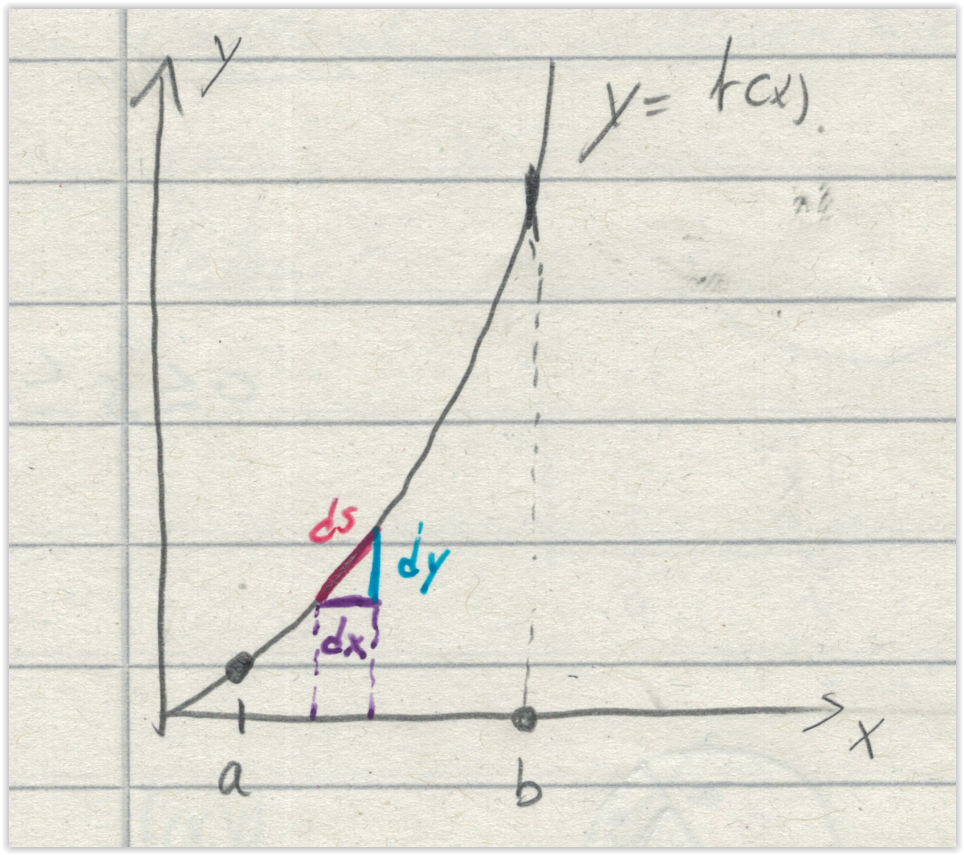
\includegraphics[width=0.4\linewidth]{./img/kurvenlaenge.png}
			  \caption{Kurvenlänge}
			  \label{fig:lkurvenlaenge}
      \end{figure}
	  \end{bem}
	  
	  \subsubsection{Flächen geschlossener ebener Kurven}
	  \begin{equation}
	    F(c) = \frac{1}{2} \int\limits_a^b \big|\big(x(t)\dot{y}(t) - y(t)\dot{x}(t)\big)\big|dt
	  \end{equation}
  \subsection{Wegintegrale}
	  \subsubsection{Wegintegral erster Art}
	  \begin{definition}
	    Das Wegintegral erster Art ist definiert durch:
	    \begin{equation}
	      \int\limits_c \varrho \; dx = \int\limits_x \varrho \; ds = \int\limits_a^b \varrho(c(t)) \quad || \dot{c}(t)|| dt \label{eq:wegintegral_1}
	    \end{equation}
	  \end{definition}
	  \begin{bem}
	    Aus \eqref{fig:wegintegral_erster_2} geht
	    \begin{equation*}
	      ds = \sqrt{dx^2 + dy^2}
	    \end{equation*}
	    hervor. Damit folgt:
	    \begin{align*}
	      ds &= \sqrt{dx^2 + dy^2} = \frac{dt}{dt}  \sqrt{dx^2 + dy^2} = \frac{1}{dt} \sqrt{dx^2 + dy^2}dt \\
	      &=  \sqrt{\frac{1}{dt^2}(dx^2 + dy^2)} =  \sqrt{\left(\frac{dx}{dt}\right)^2 + \left(\frac{dy}{dt}\right)^2}
	    \end{align*}
	    Überträgt man das bekannte Integral aus dem $\R^2$, das mit $\int\limits_a^b f(x) dx$ gegeben ist, und  obigen Zusammenhang ein, so erhält man:
	    \begin{align*}
	      \int\limits_{t=a}^{t=b} f(x,y) ds = \int\limits_{t=a}^{t=b} f(x,y) \sqrt{dx^2 + dy^2}\\
	      = \int\limits_{t=a}^{t=b} \underbrace{f(x(t),y(t))}_{\text{Höhe}} \underbrace{\sqrt{\left(\frac{dx}{dt}\right)^2 + \left(\frac{dy}{dt}\right))^2} dt}_{ds}
	    \end{align*}
	  \end{bem}
	  \begin{figure}[H] 
		\centering
		\begin{minipage}{.5\textwidth}
		  \centering
		  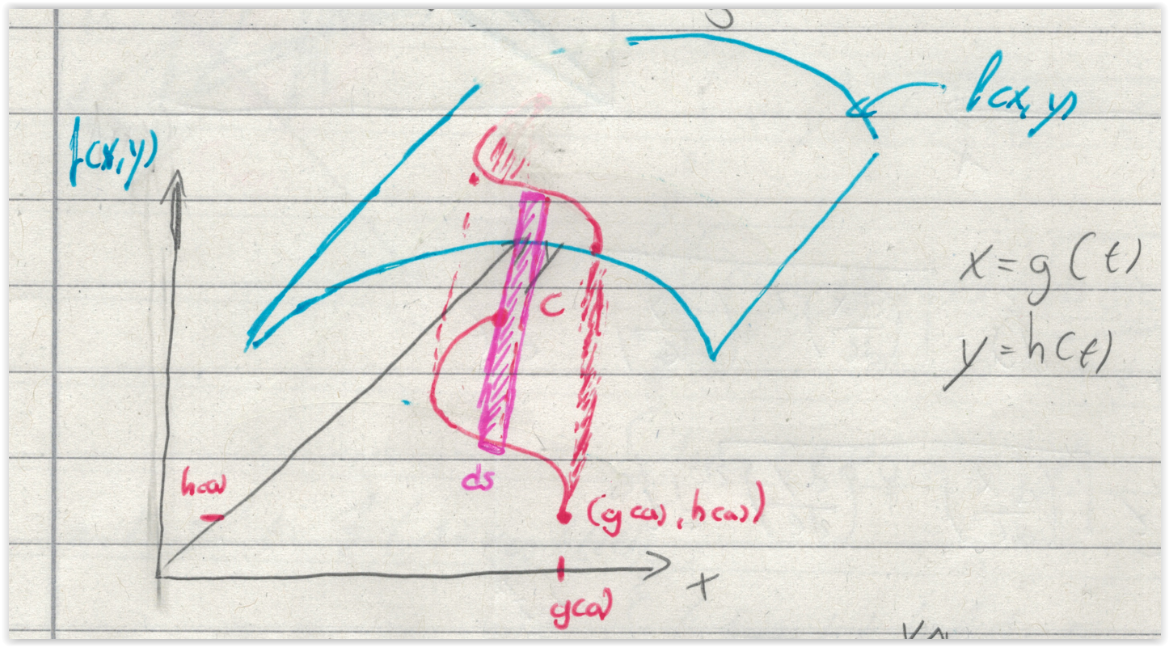
\includegraphics[width=0.9\linewidth]{./img/wegintegral_erster_1.png}
		  \caption{Graphische Interpretation}
		  \label{fig:wegintegral_erster_1}
		\end{minipage}%
		\begin{minipage}{.5\textwidth}
		  \centering
		  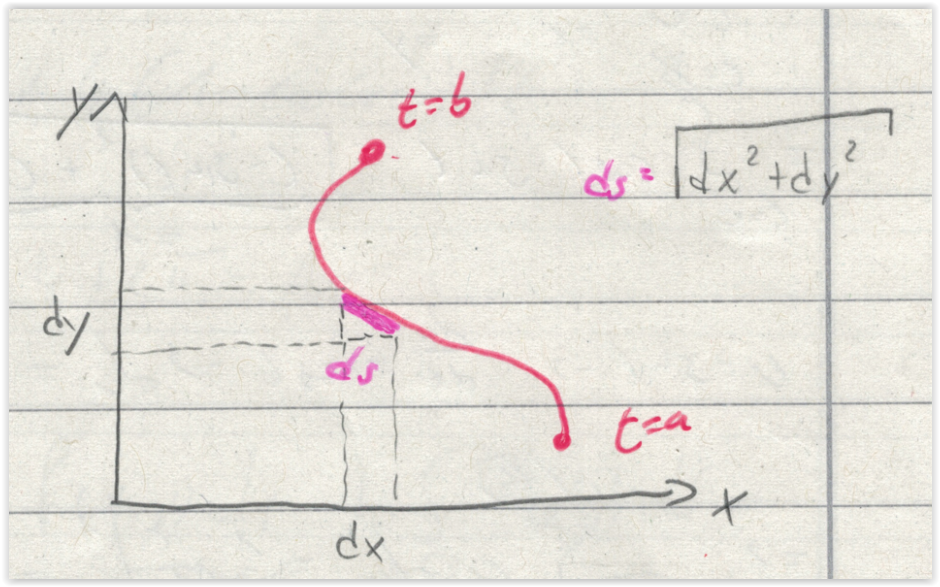
\includegraphics[width=0.8\linewidth]{./img/wegintegral_erster_2.png}
		  \caption{Interpretation von \protect\eqref{eq:wegintegral_1}}
		  \label{fig:wegintegral_erster_2}
		\end{minipage}
		\end{figure}
		\begin{bem}
			\begin{itemize}
			  \item[a) ] Integrale sind unabhängig von der gewählten Parametrisierung.
			  \item[b) ] Falls $c$ geschlossen ist so schreibt man 
				  \begin{equation}
				    \oint\limits_c \varrho \; ds
				  \end{equation}
			\end{itemize}
		\end{bem}
		\subsubsection{Wegintegrale zweiter Art}
		\begin{definition}
		  Sei $f: D\rightarrow \R^d$ ein stetiges Vektorfreld mit $D\subset \R^d$ und sei $c:[a,b] \rightarrow D$ eine stückweise $C^1$-Kurve, dann heißt 
		  \begin{equation}
		    \int\limits_c <f(x), dx> = \int\limits_a^b <f\left(c(t)\right), \dot{c}(t)>dt
		  \end{equation}
		  das Wegintegral 2-ter Art. Falls $c$ geschlossen ist schreibt man
		  \begin{equation}
		    \oint\limits_c <f(x), dx>
		  \end{equation}
		\end{definition}
		\begin{bem}
		  Das Wegintegral ist unabhängig von der gewählten Parametrisierung.
		\end{bem}
		\begin{bem}
		  Eine Alternative ältere Schreibweise ist
		  \begin{equation*}
		    \int\limits_c <f(X),dX>
		  \end{equation*}
		  Achtung, es handelt sich nur um eine Schreibweise. Nicht das Skalarprodukt aus $f(X)$ und $dX$ bilden!
		\end{bem}
		\begin{definition}
  		Ein stetiges Vektorfeld $f$ heißt wirbelfrei, falls die Kurvenintegrale längs aller stückweise stetig diffbaren Kurven verschwinden, d.h.
  		\begin{equation}
  		  \oint\limits_c <f(x), dx> = 0
  		\end{equation}
  		gilt.
		\end{definition}
		Als Konsequenz daraus folgt die Wegunabhängigkeit der Kurvenintegrale für den Fall das $f$ wirbelfrei ist. Das heißt, ist $f$ wirbelfrei, so gilt:
		\begin{equation}
		  \int\limits_{c_1} <f(x),dx> = \int\limits_{c_2} <f(x),dx>
		\end{equation}
		für beliebige Wege $c_1$ und $c_2$ mit gleichen Anfangs- und Endpunkten.
		\begin{definition}
		  Eine Teilmenge $D \subset \R^d$ heißt (weg)-zusammenhängend, falls je zwei Punkte $x,y \in D$ durch eine stückweise $C^1$-Kurve in $D$ verbunden werden können.
		  \begin{figure}[H] 
			  \centering
			  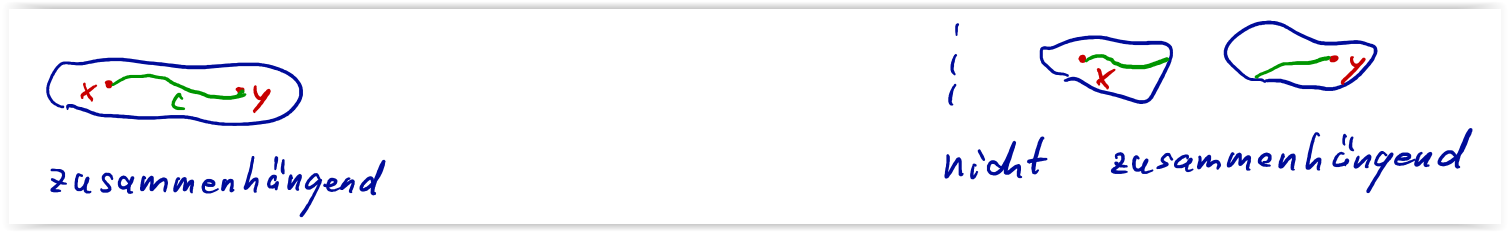
\includegraphics[width=0.8\linewidth]{./img/zusammenhaengend.png}
			  \caption{Visualisierung zusammenhängend \protect\cite{HM12}}
			  \label{fig:zusammenhängend}
		  \end{figure}
		\end{definition}
		\subsubsection{Potential}
	  \begin{definition}
	    Sei $f:D\rightarrow \R^d$ ein Vektorfeld auf $D\subset \R^d$. Wir sagen $f$ ist ein gradientenfeld, falls es eine skalare $C^1$-Funktion $\varphi: D\rightarrow\R$ gibt, mit 
	    \begin{equation}
	    \nabla \varphi(x) = f(x)
	    \end{equation}
	    $\varphi$ heißt das Potential von $f$.
	  \end{definition}
    \begin{satz}
      Sei $D \subset \R^n$ offen und zusammenhängend und $f$ ein stetiges Vektorfeld auf $D$. 
      \begin{itemize}
        \item[a) ] Besitzt $f$ ein Potential $\varphi$, so gilt für alle stückweisen $C^1$-Kurven $c$, dass 
        \begin{equation}
          \int\limits_c <f(x),dx> = \varphi(c(b)) - \varphi(c(a))
        \end{equation}
        wobei $c:[a,b]\rightarrow \R^d$. D.h. das Wegintegral ist damit wegunabhängig und $f$ wirbelfrei.
        \item[b) ] Ist $f$ wirbelfrei, so besitzt $f$ ein Potential $\varphi$ mit der Darstellung 
        \begin{equation}
          \varphi(x) = \int\limits_{c_x} f(\tilde{x}),d\tilde{x}>
        \end{equation}
        wobei $c_x$ ein Weg nach $x$ mit fest gewähltem Startpunkt $x^*$ sein soll.
      \end{itemize}
    \end{satz}	  
	  \subsubsubsection{Berechnung von Potentialen}
	  Die notwendige (aber nicht hinreichende) Bedingung für die Existenz eines Potentials ist:
	  \begin{equation}
	    rot(\nabla \varphi) = 0 \Rightarrow rot(f) = 0 \Rightarrow Potential\;ex.  
	  \end{equation}
	  \begin{definition}
	    Ein Gebiet $G$ heißt einfach zusammenhängend, falls jeder geschlossene Weg in $G$ auf einen Punkt im Gebiet zusammen gezogen werden kann.
	    \begin{figure}[H] 
			  \centering
			  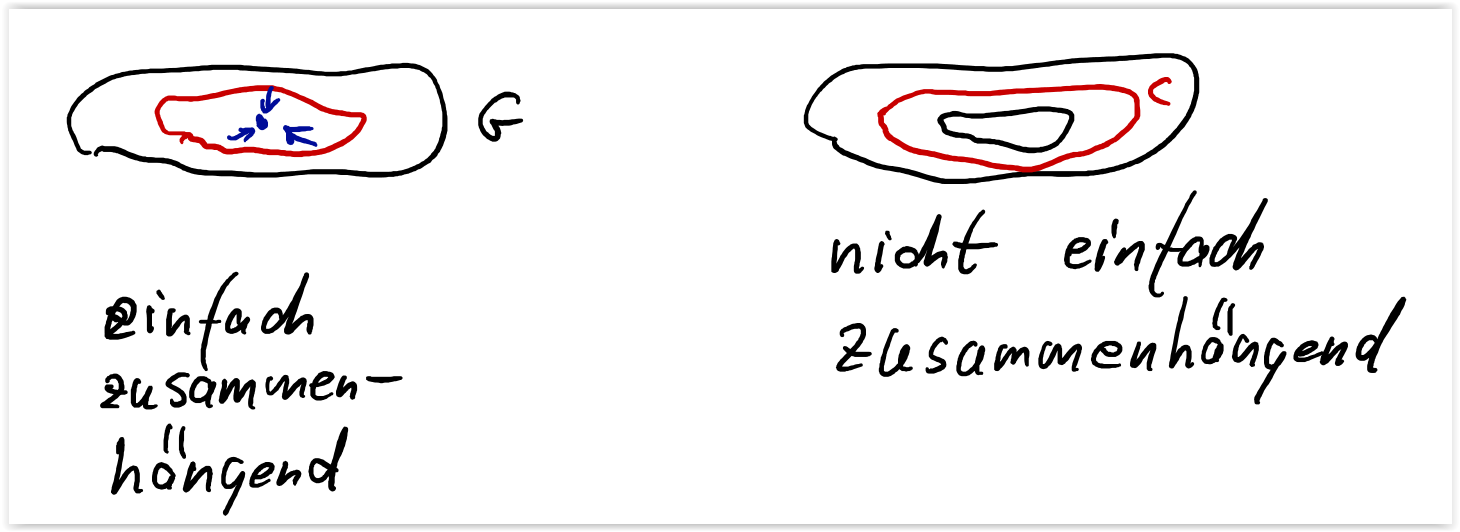
\includegraphics[width=0.8\linewidth]{./img/einfach_zusammenhaengend.png}
			  \caption{Visualisierung einfach zusammenhängend \protect\cite{HM12}}
			  \label{fig:einfach_zusammenhängend}
		  \end{figure}
	  \end{definition}
	  
  \newpage
 

\newpage
\chapter{Anhänge}
	\section{Nachwort}
Dieses Dokument versteht sich einzig als Zusammenfassung des HM3 Stoffes auf Basis der Literatur und der Vorlesungsunterlagen aus der HM3 Vorlesung von Prof. Dr. Marcel Griesemer mit einigen zusätzlichen Beispielen. Der Sinn ist einzig mir selbst und meinen Kommilitonen das studieren der Mathematik zu erleichtern. In diesem Sinne erhebe ich keinerlei Anspruch auf das hier dargestellte Wissen, da es sich in großen Teilen nur um Neuformulierungen aus der Literatur, den Vorlesungen und aus dem Begleitkurs vom Mint Kolleg handelt, in dem Frau Dr. Monika Schulz den Stoff aus der HMI und HMII bereits hervorragend zusammengefasst hat. Sollten sich einige Fehler eingeschlichen haben (was sehr wahrscheinlich ist) würde ich mich freuen, wenn man mich per Email (f.leuze@outlook.de) kontaktieren und entsprechende Fehler mitteilen würde.

\nocite{*}
\bibliography{./bib/lit}

\end{document}
